%# -*- coding: utf-8-unix -*-
%%==================================================
%% thesis.tex
%%==================================================

% 双面打印
\documentclass[master, windows, openright, twoside, english]{sjtuthesis}
% \documentclass[bachelor, openany, oneside, submit]{sjtuthesis}
% \documentclass[master, review]{sjtuthesis}
% \documentclass[%
%   bachelor|master|doctor|coursepaper, % 必选项,分别是学士,硕士,博士学位论文以及课程论文
%   fontset=fandol|windows|mac|ubuntu|adobe|founder, % 字体选项
%   oneside|twoside,        % 单面打印,双面打印(奇偶页交换页边距,默认)
%   openany|openright,      % 可以在奇数或者偶数页开新章|只在奇数页开新章(默认)
%   english,                % 启用英文模版
%   review,     % 盲审论文,隐去作者姓名、学号、导师姓名、致谢、发表论文和参与的项目
%   submit      % 定稿提交的论文,插入签名扫描版的原创性声明、授权声明
% ]


% 逐个导入参考文献数据库
\addbibresource{bib/thesis.bib}

%# -*- coding: utf-8-unix -*-
% !TEX program = xelatex
% !TEX root = ../thesis.tex
% !TEX encoding = UTF-8 Unicode
%TC:ignore
\title{COMPETITION OF SOCIAL OPINIONS ON TWO LAYER NETWORKS}
\author{HYUNCHEL CHO}
\advisor{王琳教授}
% \coadvisor{某某教授}
\defenddate{2020年 2月00日}
\coursename{控制工程}
\school{上海交通大学}
\institute{电子信息与电气工程学院}
\studentnumber{117032990005}
\cnacademicdegree{工学硕士}
\major{控制科学与工程}
\keywords{complex network, interconnected network, modeling and simulation, social network analysis, opinion dynamics, consensus, language competition dynamics}

\englishtitle{Competition of Social Opinions on Two Layer Networks}
\englishauthor{HYUNCHEL CHO}
\englishadvisor{Prof. Wanglin}
% \englishcoadvisor{Prof. \textsc{Uom Uom}}
\englishschool{Shanghai Jiao Tong University}
\englishinstitute{\textsc{School of Electronic Informatioin and Electrical Engineering} \\
  \textsc{Shanghai Jiao Tong University} \\
  \textsc{Shanghai, P.R.China}}
\englishinstitutemaster{School of Electronic Informatioin and \\ Electrical Engineering}
\englishmajor{Control Science and Engineering}
\englishdate{Jan. 17th, 2020}
\enacademicdegree{Master of Engineering}
\englishstudentid{117032990005}
\englishkeywords{opinion dynamics, competition, consensus}
%TC:endignore
  % NOTE: the enclosed commands must be executed in preamble
\setcounter{tocdepth}{1}

\begin{document}
	
% 无编号内容:中英文论文封面、授权页
\maketitle
\makeatletter

\ifsjtu@coursepaper
\else
  \ifsjtu@submit\relax
    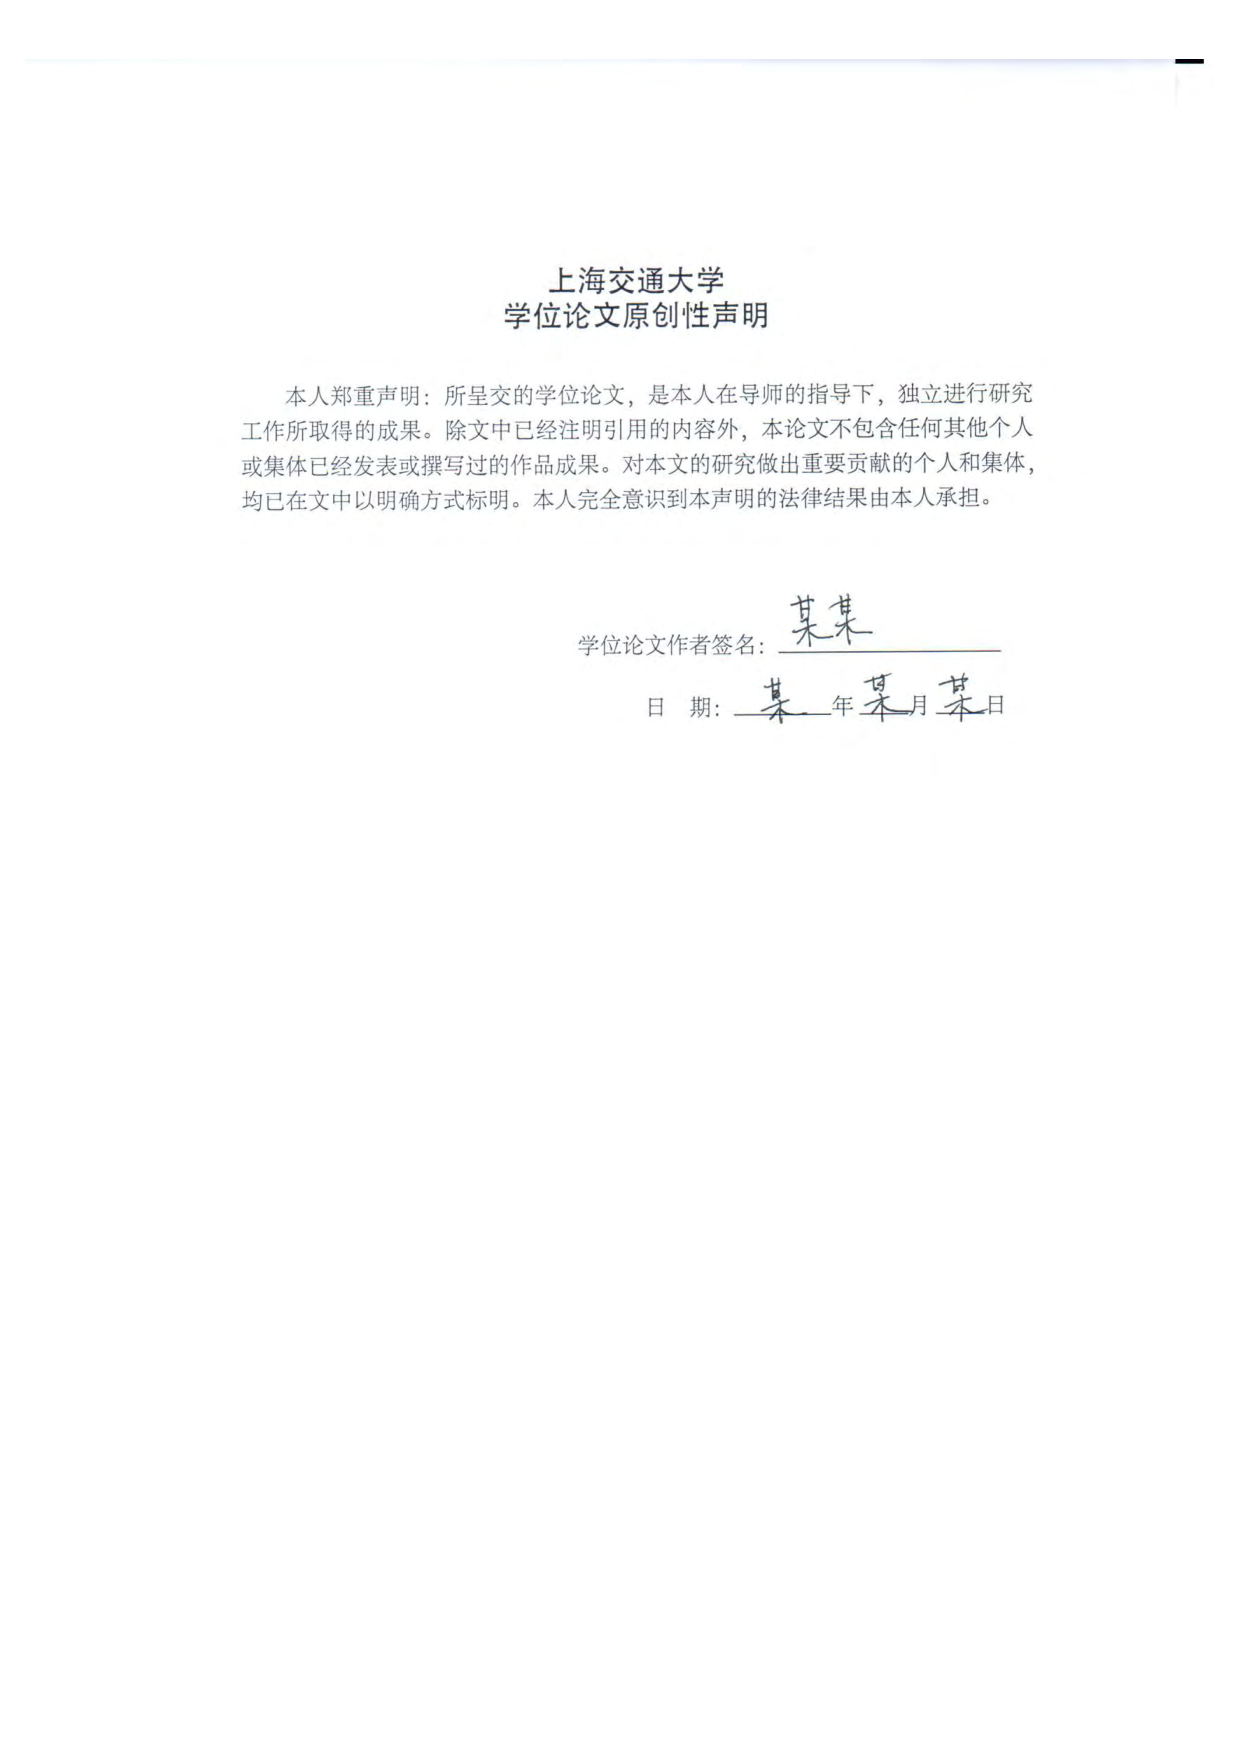
\includepdf{pdf/original.pdf}
    \cleardoublepage
    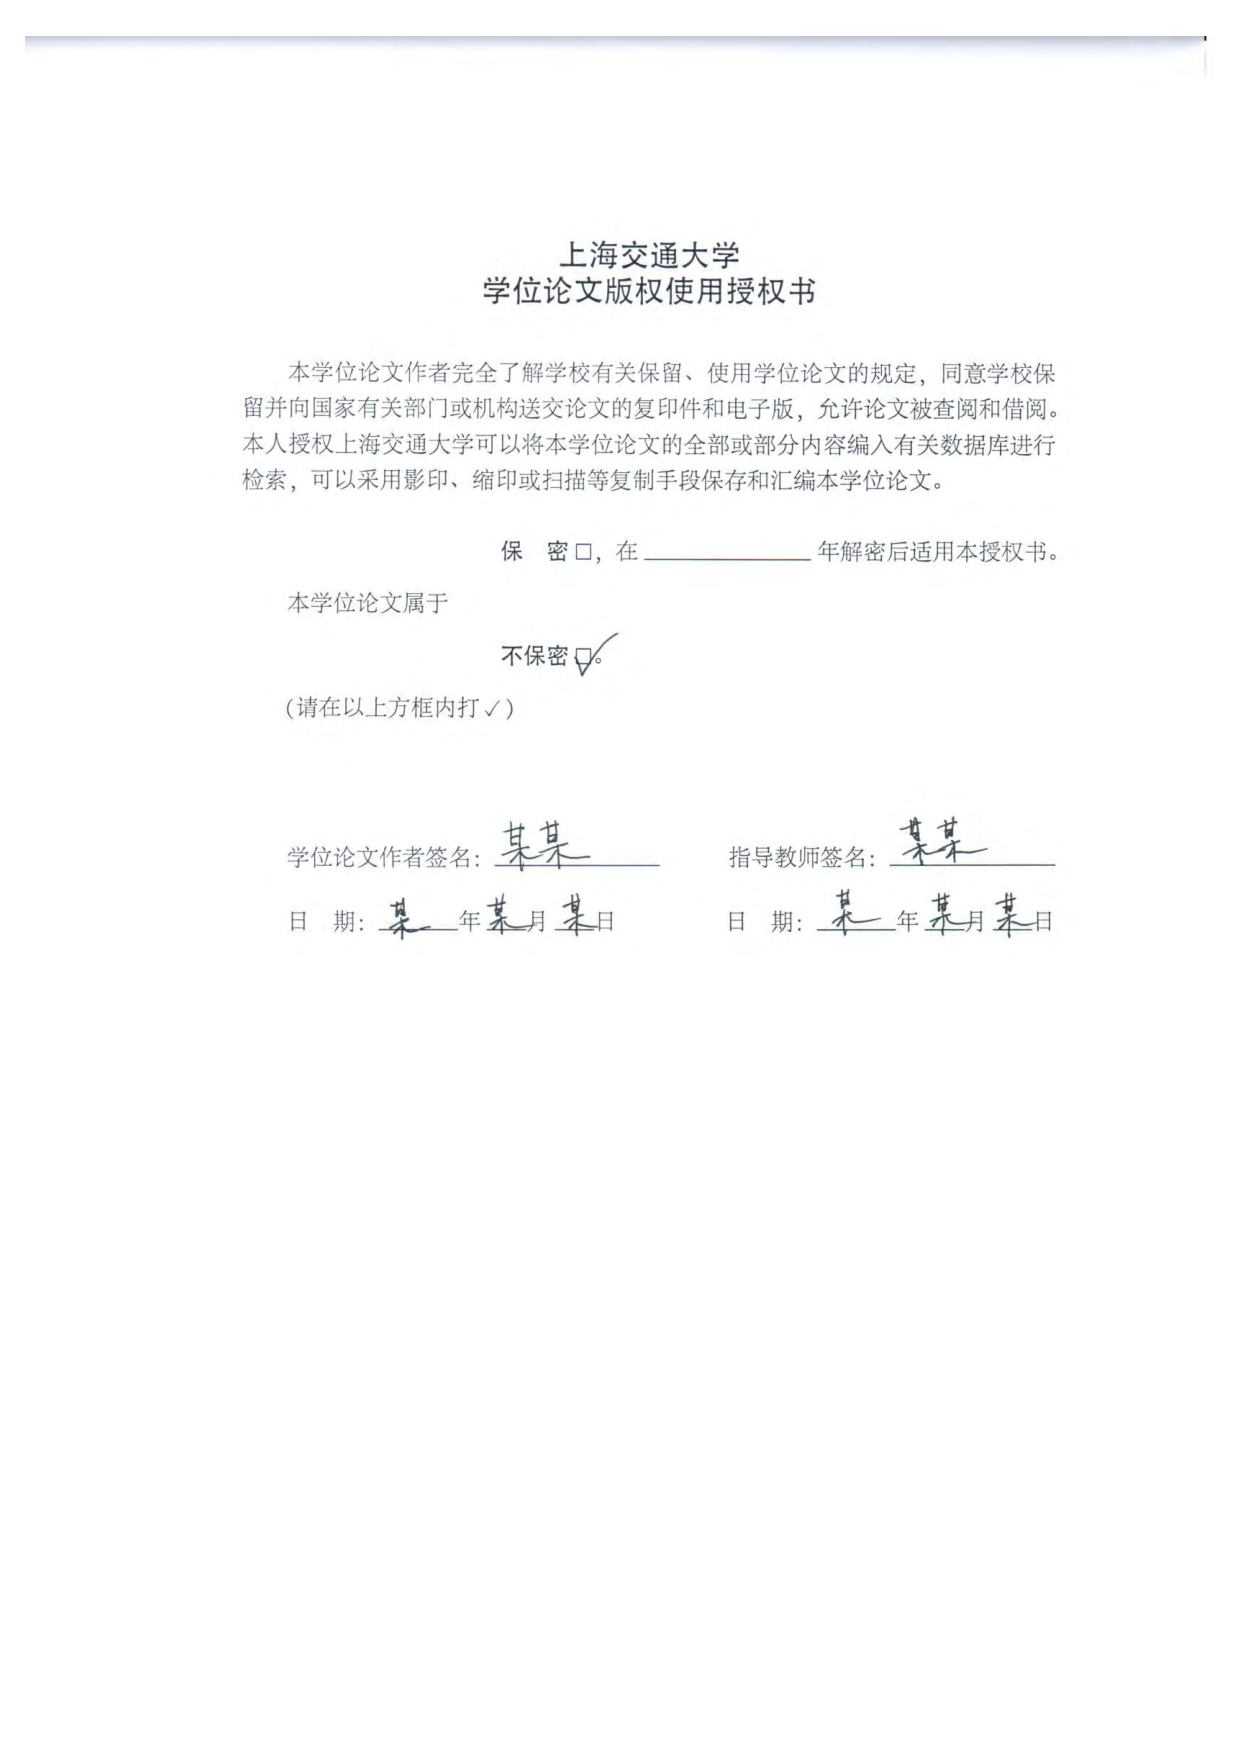
\includepdf{pdf/authorization.pdf}
    \cleardoublepage
  \else
    \ifsjtu@review\relax
    % exclude the original claim and authorization
    \else
      \makeDeclareOriginal
      \makeDeclareAuthorization
    \fi
  \fi
  \frontmatter % 使用罗马数字对前言编号

  % 摘要
  %# -*- coding: utf-8-unix -*-
% !TEX program = xelatex
% !TEX root = ../thesis.tex
% !TEX encoding = UTF-8 Unicode
%%==================================================
%% abstract.tex for SJTU Master Thesis
%%==================================================

\begin{abstract}
	
在诸如社会问题探讨、总统竞选投票等问题上,不同的群体通常会有不同的意见,竞争是不可避免的。社会舆论竞争一直是复杂网络和社会行为学的研究热点。本文研究了双层网络中的竞争,以及网络结构、更新规则以及关键节点对竞争结果的影响。

首先,采用双层网络对两个群体的竞争进行建模,其中A层为意见形成组,B层为决策组。初始极化竞争状态设置为A层节点均持正面观点,B层节点均持负面观点,分析了网络结构、内部度和外部度对竞争状态的影响。仿真结果表明,内外部连边在竞争中都起着至关重要的作用。值得注意的是,增加某层的内部连边和外部连边,可以更容易战胜另一个群体并最终达成共识。

其次,基于双层意见模型,研究了更新规则对竞争的影响。从层、节点、边等不同角度,考虑了更新规则,包括顺序更新规则和同步更新规则。实验表明,同步更新规则更容易使网络达到共存状态并且容易被改变为相反状态,而顺序更新规则可以更快地达成共识。

此外,通过固定一些关键节点在观点演化中的状态,研究了其对竞争的影响。利用Pagerank、度中心性、特征向量中心性、介数中心性、接近中心性等中心性指标及其组合选择关键节点。通过仿真发现关键节点的影响因网络结构和观点动态而不同。此外,使用单中心性指标和多中心性指标的方法选取出的关键节点,都能很好地说服其他群体的节点改变观点。 \\ 

\end{abstract}


\begin{englishabstract}
	
Different groups usually have different opinions, such as opposite opinions during votes on social issues, presidential campaigns, and so on, where competition is unavoidable. Competition on the interconnected networks has always been a hot topic in the fields of complex networks and social behaviors. In this paper, we investigate competitions in a two-layer network and study the influence of network structures, updating rules as well as key nodes on the competition results.

First, the influence of network structures is studied by switching internal degrees, external degrees and network types. A two-layer network is used to model the competition of two groups, where layer A is an opinion formation group, and layer B is a decision-making group. Starting with a polarized competition state, where all nodes in layer A have positive opinions while all nodes in layer B have negative opinions, the state of a network is changed through the evolution of opinions. Various network structures are simulated and analyzed. Simulation results show that both internal and external links play vital roles in the competition. Notably, increasing the number of external and internal links on one layer can make it easy to prevail over the other group and reach consensus.

Second, the influence of updating rules is investigated based on the previous two-layer opinion model. The updating rules, including sequential order and simultaneous order, are considered according to different levels, such as layers, nodes, and edges. It is observed that a simultaneous updating rule is more likely to make the state of the network have a coexistence state and easily be changed to the opposite state, while a sequential updating rule can enable consensus more quickly.

Moreover, the influence of critical nodes on the competition is studied by fixing their states during the evolution of opinion. Some centrality indexes, including Pagerank, degree, eigenvector, betweenness, closeness, and their combinations, are used to select the key nodes. Through simulations, it is found that the influence of the key nodes is different according to network structures and opinion dynamics. Besides, both single centrality and multiple centralities have an excellent performance for selecting key nodes, so that the selected critical agents persuade the other group of agents to change their opinion more quickly.\\ 

\end{englishabstract}



  % 目录、插图目录、表格目录
  \tableofcontents
  \listoffigures
  \addcontentsline{toc}{chapter}{\listfigurename}     % 将插图目录加入全文目录
  \listoftables
  \addcontentsline{toc}{chapter}{\listtablename}      % 将表格目录加入全文目录
  %\listofalgorithms
  %\addcontentsline{toc}{chapter}{\listalgorithmname}  % 将算法目录加入全文目录

  %%# -*- coding: utf-8-unix -*-
% !TEX program = xelatex
% !TEX root = ../thesis.tex
% !TEX encoding = UTF-8 Unicode
%TC:ignore
\begin{nomenclaturename}
\label{chap:symb}

\begin{longtable}{rl}
$\epsilon$     & 介电常数 \\
 $\mu$ 		& 磁导率 \\
 $\epsilon$     & 介电常数 \\
 $\mu$ 		& 磁导率 \\
 $\epsilon$     & 介电常数 \\
 $\mu$ 		& 磁导率 \\
 $\epsilon$ 	& 介电常数 \\
 $\mu$ 		& 磁导率 \\
 $\epsilon$     & 介电常数 \\
 $\mu$ 		& 磁导率 \\
 $\epsilon$     & 介电常数 \\
 $\mu$ 		& 磁导率 \\
 $\epsilon$     & 介电常数 \\
 $\mu$ 		& 磁导率 \\
 $\epsilon$ 	& 介电常数 \\
 $\mu$ 		& 磁导率 \\
 $\epsilon$     & 介电常数 \\
 $\mu$ 		& 磁导率 \\
 $\epsilon$     & 介电常数 \\
 $\mu$ 		& 磁导率 \\
 $\epsilon$     & 介电常数 \\
 $\mu$ 		& 磁导率 \\
 $\epsilon$ 	& 介电常数 \\
 $\mu$ 		& 磁导率 \\
 $\epsilon$     & 介电常数 \\
 $\mu$ 		& 磁导率 \\
 $\epsilon$     & 介电常数 \\
 $\mu$ 		& 磁导率 \\
 $\epsilon$     & 介电常数 \\
 $\mu$ 		& 磁导率 \\
 $\epsilon$ 	& 介电常数 \\
 $\mu$ 		& 磁导率 \\
 $\epsilon$     & 介电常数 \\
 $\mu$ 		& 磁导率 \\
 $\epsilon$     & 介电常数 \\
 $\mu$ 		& 磁导率 \\
 $\epsilon$     & 介电常数 \\
 $\mu$ 		& 磁导率 \\
 $\epsilon$ 	& 介电常数 \\
 $\mu$ 		& 磁导率 \\
 $\epsilon$     & 介电常数 \\
 $\mu$ 		& 磁导率 \\
 $\epsilon$     & 介电常数 \\
 $\mu$ 		& 磁导率 \\
 $\epsilon$     & 介电常数 \\
 $\mu$ 		& 磁导率 \\
 $\epsilon$ 	& 介电常数 \\
 $\mu$ 		& 磁导率 \\
 $\epsilon$     & 介电常数 \\
 $\mu$ 		& 磁导率 \\
 $\epsilon$     & 介电常数 \\
 $\mu$ 		& 磁导率 \\
 $\epsilon$     & 介电常数 \\
 $\mu$ 		& 磁导率 \\
\end{longtable}

\end{nomenclaturename}
%TC:endignore
 % 主要符号、缩略词对照表
\fi

\makeatother
\mainmatter % 使用阿拉伯数字对正文编号

% 正文内容
%# -*- coding: utf-8-unix -*-
% !TEX program = xelatex
% !TEX root = ../thesis.tex
% !TEX encoding = UTF-8 Unicode
%%==================================================
%% chapter01.tex for SJTU Master Thesis
%%==================================================

%\bibliographystyle{sjtu2}%[此处用于每章都生产参考文献]
\chapter{Introduction}
\label{chap1}
\section{Introduction}
People have their own opinions, and sometimes they change their opinions in response to others who have views on those issues. Their opinions are reflected in the leaders to make laws and make necessary decisions. These phenomena can be found in some cases, such as voting, legislation, and the adoption of new policies. It is widely recognized that both opinion formation and decision-making formation have mutual interaction as interconnected networks.\parencite{mikko2014, danziger2019, newman2010, boccaletti2014, domenico2013, tomasini2015, namkhanhvu2017}. Sometimes, opinion formation could be opposed to decision-making formation. These situations often give rise to social conflicts and confusion. In order to figure out these social conflicts, it is necessary to understand and analyze the competition of interconnected networks. So far, physics and computer science have researched these social conflicts by modeling and analyzing complex systems\parencite{fangwu2004, zuev2012, laguna2004, masuda2014}. The researches include opinion dynamics, voter model, game theory, and many more.\parencite{smyrnakis2019, bianconi2018, redner2017, haibo2017, amato2017, quattrociocchi2014, casey2009} 
Competition of interconnected networks has been researched in various ways. These networks can be applied to the dissemination of computer viruses, messages, opinions, memes, diseases, and rumors\parencite{hua2014,shenyu2018, zhou2018, alvarez2016,gomez2015,diep2017,rocca2014,velasquez2018}. Opinion dynamics on interconnected networks has been investigated with various network models such as \textit{Abrams-Strogatz(AS)} model\parencite{abrams2003,vazquez2010} and $M$ model\parencite{rocca2014}.  Based on the previous research, this work studies the main features of competition in two-layer networks by changing network structures, changing the updating rules, and selecting the key nodes. It is proven and analyzed that these different conditions cause different results.
\begin{figure}[!htb]
	\centering
	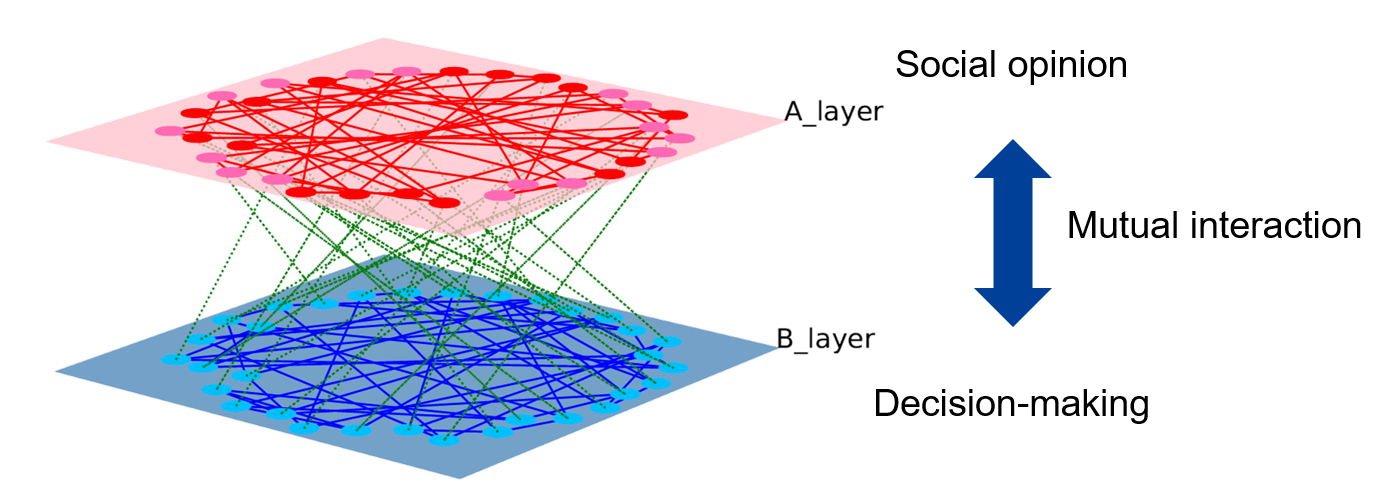
\includegraphics[width=\hsize]{chap1_topic.png}
	\caption{The example of competition on the two-layer network}
	\label{chap1_topic}
\end{figure}

\section{Competition on interconnected networks}
In this research, we focus on the competition on a two-layer network or an interconnected network. If compared with a single-layer network, the interconnected network has two dynamics, two parameters, and includes internal edges and external edges, as shown in Fig.~\ref{chap1_singlemulti}. Therefore, the interconnected network interaction is more complex than single-layer network interaction.

\begin{figure}[!htb]
	\centering
	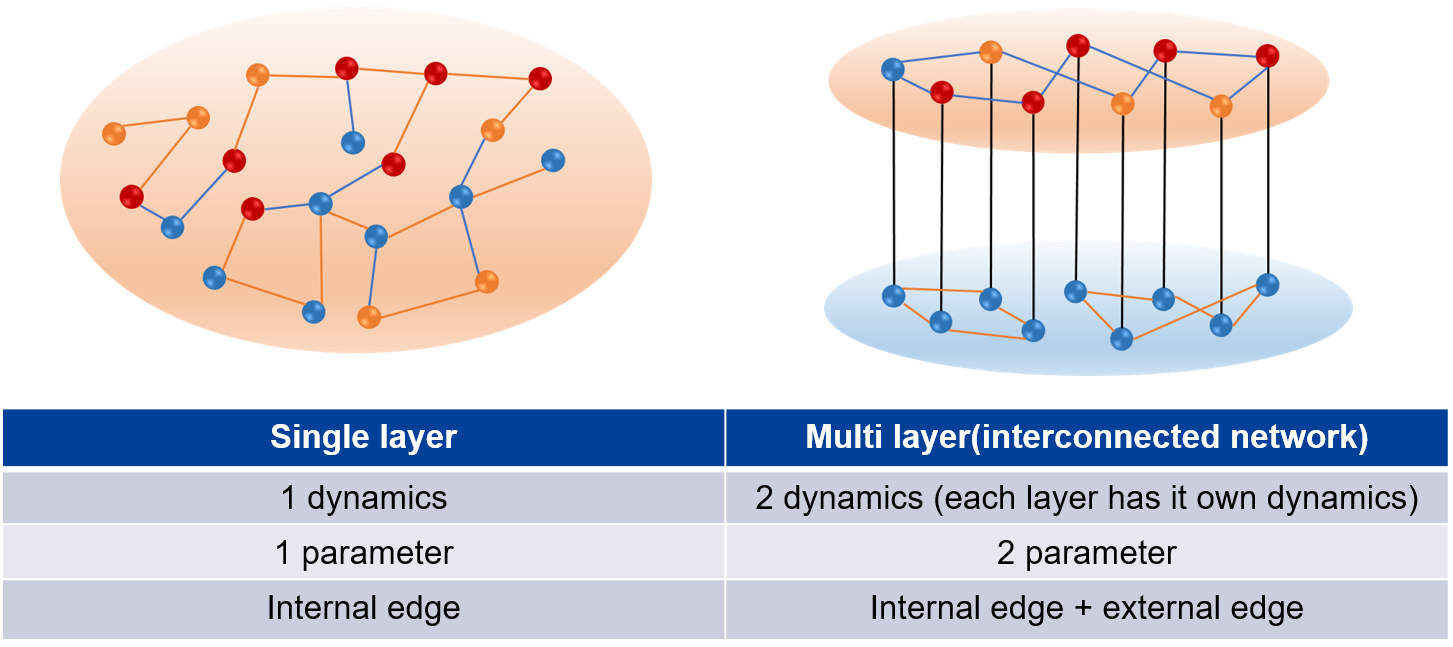
\includegraphics[width=\hsize]{chap1_singlemulti.png}
	\caption{Comparison between a single-layer network and a two-layer network}
	\label{chap1_singlemulti}
\end{figure}

In order to make a two-layer network under competition, each layer is made up of different dynamics and parameters. Network dynamics are based on previous research, such as \parencite{alvarez2016}. The top layer has the function of social opinion and its dynamics. Some opinion models provide a social mechanism through the compromise process.\parencite{naim2003} Other opinion models represent the persuasive process.\parencite{chau2014} In this research, the social opinion layer is affected by the opinion dynamics, which are also known as M-model\parencite{rocca2014}, which includes compromise function and persuasion function. The bottom layer has the function of decision-making and its dynamics. The dynamics of the decision-making layer is the language competition dynamics that are also called as the \textit{Abrams-Strogatz} model\parencite{abrams2003, vazquez2010, patriarca2012}. This model is useful to decide only one opinion from two opinions. In order to make the competition condition of these two layers, the initial states of the two layers are assumed to be in opposite states, that the social opinion layer has all positive states and the decision-making layer has all negative states.

So far, main researchers have focused on what factors make a consensus or dissent(coexistence), which have shown that the system can make positive consensus, negative consensus, or coexistence under a certain range of parameters, such as volatility, reinforcement, and prestige.\parencite{alvarez2016} Moreover, the interconnected competition of the social network has been researched by finding the threshold or critical point for consensus.\parencite{alvarez2016, gomez2015, diep2017} Also, it has been found out that the thresholds make the transition of states, and they can explain and analyze the social phenomena in the real world, such as the legislation, election, and social conflicts.\parencite{alvarez2016, amato2017, diep2017}

In \parencite{gomez2015}, it is shown that the transition from localized to mixed status occurs through a cascade from poorly connected nodes in the layers to the highly connected ones and the external degree is critical to change the state of the network. Besides, the main features, such as transition and cascade, found in Monte Carlo simulation, are precisely characterized by the mean-field theory and magnetization\parencite{alvarez2016, diep2017, amato2017, gomez2015}. 

Based on all this previous research, the competitions of interconnected networks are analyzed by three main topics, such as network structures, updating rules, and selection of key nodes. Before simulations, backgrounds for three topics are explained as follows. 
\begin{figure}[!htb]
	\centering
	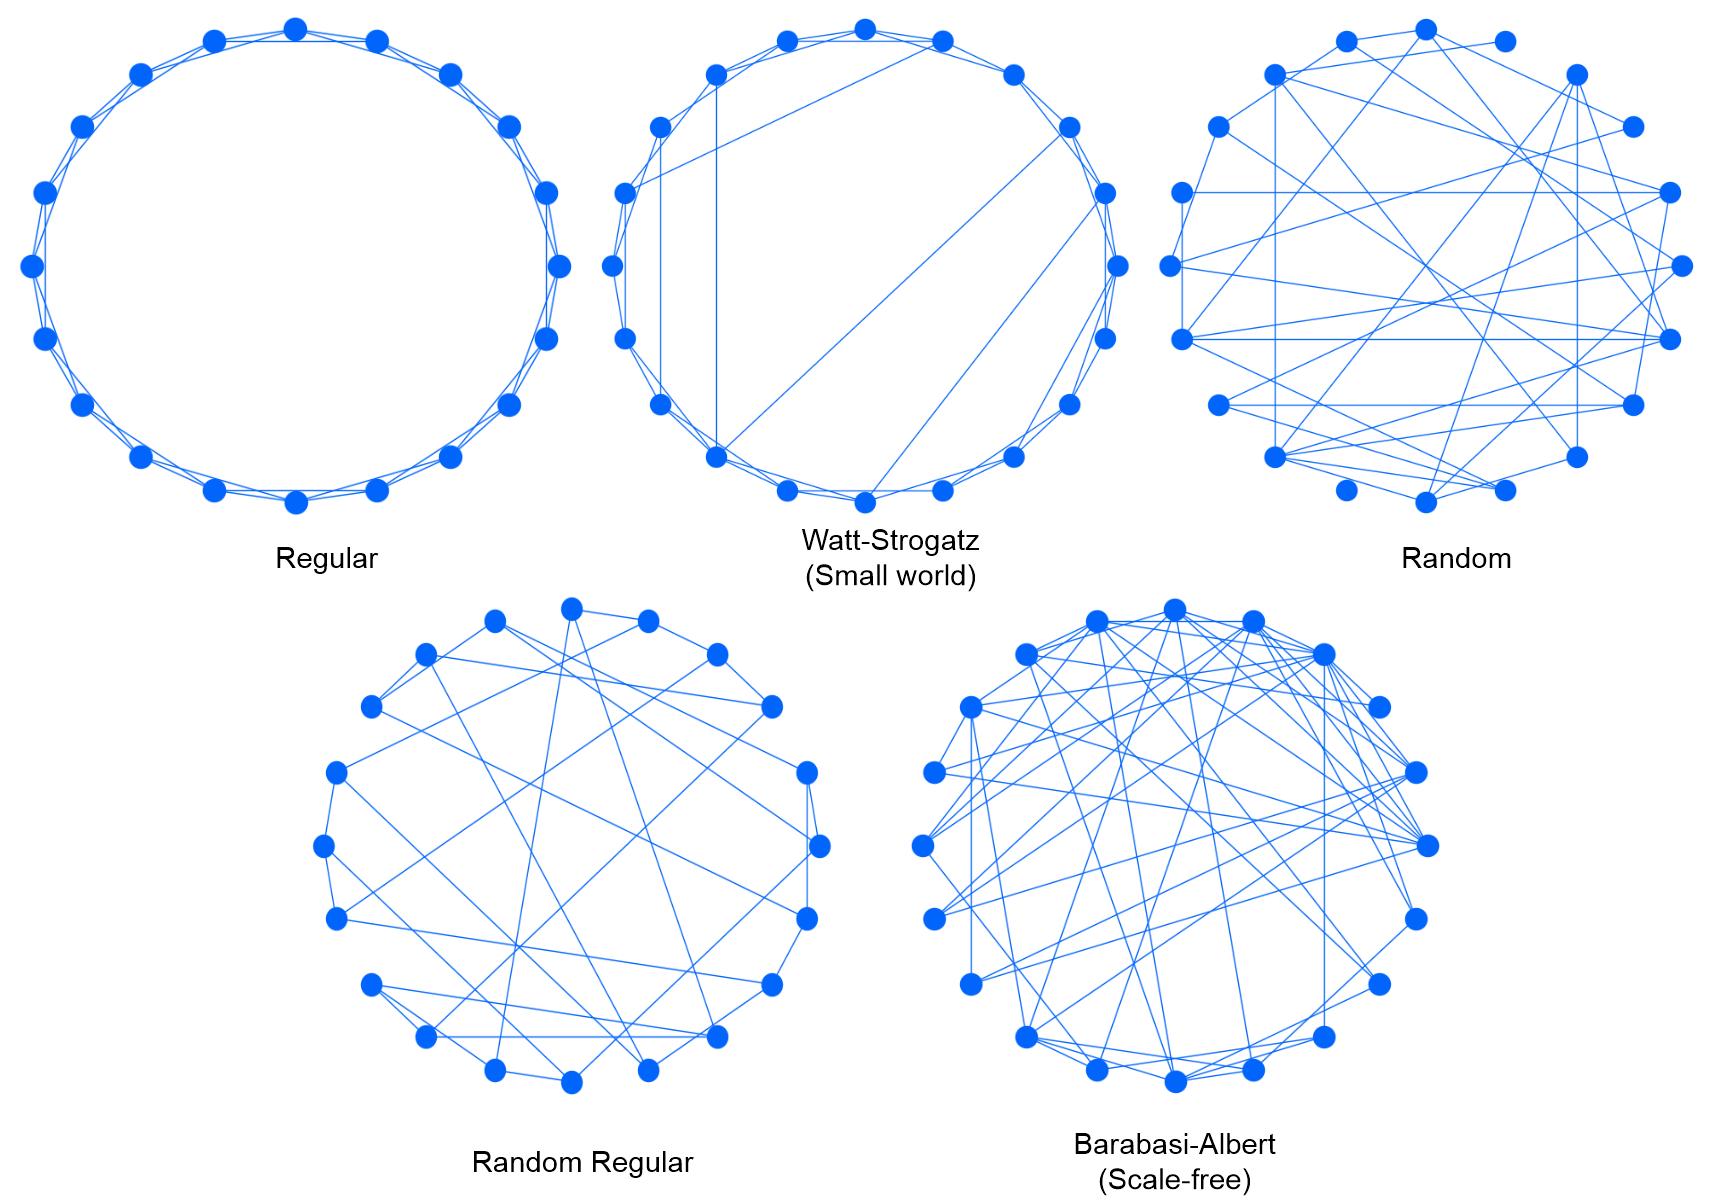
\includegraphics[width=\hsize]{chap1_network_type.png}
	\caption{Various structures of the network}
	\label{chap1_network_type}
\end{figure}
First, network structures are investigated. Networks can be largely divided into a regular network, random network\parencite{erdos1960}, small-world network\parencite{watts1998}, scale-free network\parencite{barabasi1999}, and others. Fig.~\ref{chap1_network_type} shows the structures of various networks. A regular network has a lattice structure, and each node has the same number of links. A random network is made up of edges such that two nodes are connected with probability $p$ in the systems with $K$ nodes. A small-world network is a network graph in which most nodes are not neighbors of one another, but most nodes can be reached from every other node by a small number of links. A small-world network can be made by eliminating the edges with probability $p$ and connecting two random nodes that are not connected in a regular network. A small-world network has all characteristics of a regular network and random network. A scale-free network has a model such that the distribution of edges follows power function. Examples of a scale-free network are the World Wide Web (WWW), the Internet, movie star networks, protein interactions, metabolism, and so on. There are several ways to create a scale-free network. Among them, the most typical way is the \textit{Barabasi-Albert} model. The \textit{Barabasi-Albert} model is growing networks in which nodes continue to be added, and connections between nodes have a preferential attachment. The process of creating this model repeats the following two processes: First, add one node with a constant number of edges to the system. Second, edges of the added nodes are connected in proportion to the edge number of the pre-existing nodes. In this work, two types of general networks are applied, such as a random regular(RR) network and \textit{Barabasi-Albert}(BA) network. 

Second, dynamics orders and updating rules are also studied. For further understanding of the competition on a two-layer network, it is crucial to investigate the interaction between nodes or layers. Methods of interaction between nodes are various.\parencite{sirbu2017} However, related to time, the types of interactions would be divided into two categories, such as simultaneous interaction, and sequential interaction. In economics and social networks, it has been proven that there exist different results between simultaneous and sequential interaction.\parencite{hoffman2011, dietrich2004} In \parencite{hoffman2011}, it was researched how experimental subjects update induced prior information when receiving two information signals simultaneously or receiving the same signals sequentially. As the experimental results, the simultaneous treatment is very different from sequential treatment, and under sequential information,  subject’s mean estimates of the two treatments(good news preceding bad news or vice versa) are also significantly different from each other. In conclusion, both the sequencing of process and the order of information matters. Moreover, in \parencite{dietrich2004}, the usual random sequential updating rule is replaced by the simultaneous updating rule on the \textit{Sznajd} model. It is found out that this change makes a complete consensus much more difficult. The reason is analyzed as some agents with the simultaneous updating rule receive conflicting messages from different neighbor pairs and thus refuse to change their opinion. In this work, both simultaneous and sequential updating rules are applied to layers, nodes, and links.

Third, network centralities would be researched to select key nodes on a two-layer network. Network centrality means the index to measure how close each node is to the center of a network. That answers the question, "What characterizes an important node?". The concept of network centrality was first introduced in the field of social network analysis.\parencite{freeman1979} After that, it has expanded to various areas where the concept of the network is related and has been used to identify which nodes are important in the network. So far, various criteria for assessing network centrality have been presented. Generally, well-known network centralities include degree centrality, betweenness centrality, closeness centrality, eigenvector centrality, and Pagerank.\parencite{koschutzki2008, francisco2019, bianconi2018} Degree centrality is the simplest but the most reliable concept. It is defined as the number of interacting neighbor nodes (or edges). Betweenness centrality is the concept of using the shortest path between two nodes on a network. It is explained as the concept to define two different node sets on the network (set $1$, $2$) and quantify how often each node appears on the shortest path for all combinations of nodes in set $1$ and set $2$. Closeness centrality is derived from that the shorter the path that one node reaches all the other nodes is, the more influential the node is. Eigenvector centrality is the concept that the more a node is connected with critical nodes, the more critical it is. Pagerank measures the convergent value by repeating the process of propagating each node's influence on the other nodes.
So far, many researchers have tried to select critical nodes in a social network.\parencite{eom2015, white2003, mesgari2015, hwang1981, huang2014} Based on a node centrality, some algorithms for identifying key nodes has been found out. In \parencite{mesgari2015, huang2014}, it has been found out that optimally combining multiple measures of nodal importance may provide a robust tool for identifying key nodes of interest, particularly in large graphs. Here, based on previous research, we select the key nodes by using a single node centrality and combined node centrality.

In this work, for single indicator methods to select key nodes, network centralities would be applied, such as Pagerank, degree, eigenvector, betweenness, and closeness. As multiple indicator methods recognize key nodes, several combined node centralities are applied, such as \textit{PR+DE, PR+BE, DE+BE, PR+DE+BE} that are based on single indicators.  By using these centralities(Pagerank, degree, eigenvector, closeness, betweenness, and combined node centralities), it is discussed and shown that which method is the most influential for changing the state of network on various models.\\  

\section{Motivation and organization}

In this work, opinion dynamics of a competing two-layer social network would be investigated based on the pre-existed research\parencite{alvarez2016, gomez2015, diep2017, rocca2014}. We develop modeling and research to find out the characteristics of interconnected networks. 

This research has four main directions to investigate the features of the competition model. First, it is shown how to make up competition models and how to measure the consensus for analysis. Second, we find out what factors make consensus by changing network structures. Third, it is analyzed how dynamics orders and updating rules influence the state of the two-layer network. Fourth, based on network centralities, it would be investigated which method is the most effective to identify key nodes.

This study can help to explain social network phenomena, such as a social conflict between two opinions. Therefore, this research can be used as a tool for making an efficient decision-making system, solving the social conflict, and analyzing social network problems such as legislation and vote system.

This paper is organized as follows. In the chapter~\ref{chap2}, it is introduced to how competition model of two-layers is made up and how the dynamics of each layer works. Moreover, some indexes are provided to measure and evaluate the simulation results. In the chapter~\ref{chap3}, with changing network structure, it is shown how the network structures influence the consensus of the two-layer network. In the chapter~\ref{chap4}, considering the dynamics orders and updating rules, simulation results are compared and analyzed. In the chapter~\ref{chap5}, it is researched which nodes are critical for affecting the state of the network by using single indicators and multiple indicators. Finally, in the chapter~\ref{chap6}, all simulation results are summarized, and our findings are concluded. \\



%# -*- coding: utf-8-unix -*-
% !TEX program = xelatex
% !TEX root = ../thesis.tex
% !TEX encoding = UTF-8 Unicode
%%==================================================
%% chapter02.tex for SJTU Master Thesis
%% based on CASthesis
%% modified by wei.jianwen@gmail.com
%% Encoding: UTF-8
%%==================================================

\chapter{A two-layer network model}
\label{chap2}
In this chapter, a basic model is introduced for competition on a two-layer network. It is also described that how each layer is made up and what kind of function and dynamics it has. Also, several indexes are provided to analyze and measure the interaction between two-layers.
\begin{figure}[!htb]
	\centering
	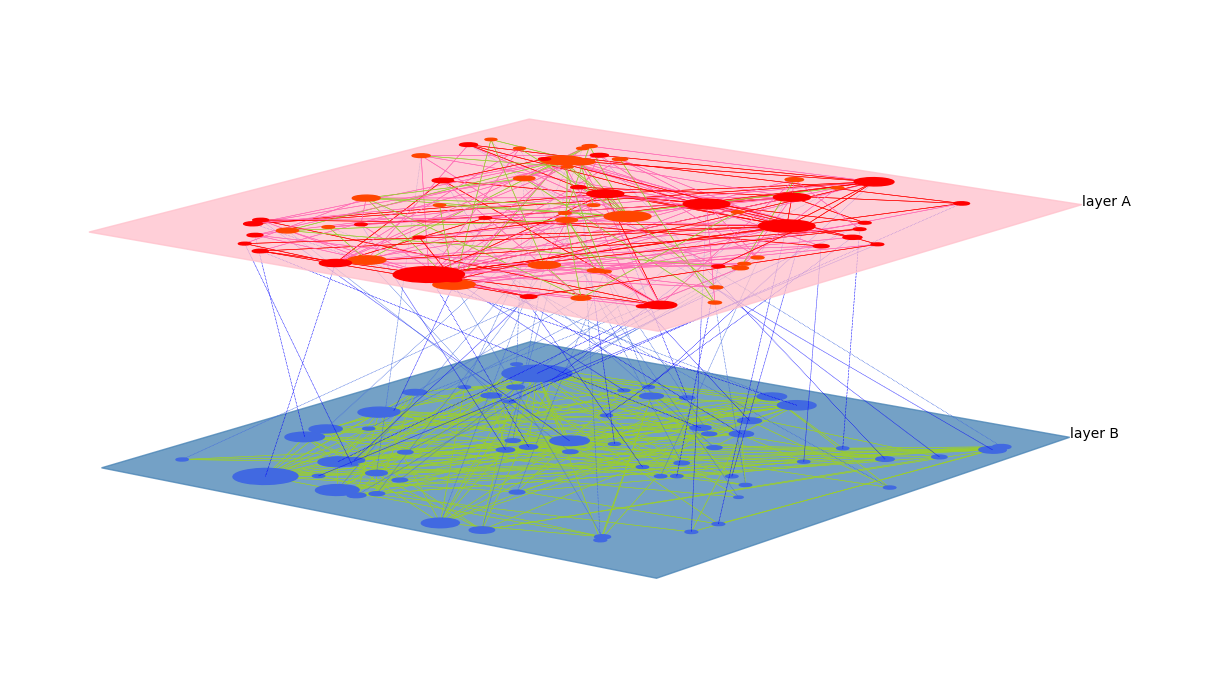
\includegraphics[width=\hsize]{chap2_modeling.png}
	\caption{Competition of Interconnected Network}
	\label{chap2_modeling}
\end{figure}
 
\section{Modeling of a two-layer network}
\label{sec:modeling of two layer network}
The model consists of two layers, and each layer has different dynamics. For layer A, the node changes its state according to the $M$ model, as introduced in \parencite{rocca2014}. Here, we choose $M=2$, that each node can have one of four states $(-2, -1, +1, +2)$. For each link $(k, j)$ belong to layer A, the dynamics are designed as follows:
\begin{itemize}
	\item Compromise: if two nodes connected with link$(k, j)$ have opposite orientations, their states become more moderate with probability $q$ :
	\begin{align}
	\mbox{if } S_k<0 \mbox{ and } S_j>0  \Rightarrow (S_k, S_j) \rightarrow (S_k^r, S_j^l) \mbox{ with } prob.q,\\
	\mbox{if } S_k>0 \mbox{ and } S_j<0  \Rightarrow (S_k, S_j) \rightarrow (S_k^l, S_j^r) \mbox{ with } prob.q.
	\end{align}
	If $S_k = \pm1$ and $S_j = \mp1$, one switches orientation at random:
	\begin{align}
	(\pm 1, \mp 1)\rightarrow \left\{\begin{matrix}
	(+1, +1) \mbox{ with } prob.q/2,
	\\(-1, -1)\mbox{ with } prob.q/2.
	\end{matrix}\right.
	\end{align}
		
	\item Persuasion: if two nodes connected with link$(k, j)$ have the same orientation, their states become more extreme with probability $p$ :
	\begin{align}
	\mbox{if } S_k<0 \mbox{ and } S_j<0  \Rightarrow (S_k, S_j) \rightarrow (S_k^l, S_j^l) \mbox{ with } prob.p,\\
	\mbox{if } S_k>0 \mbox{ and } S_j>0  \Rightarrow (S_k, S_j) \rightarrow (S_k^r, S_j^r) \mbox{ with } prob.p.
	\end{align}
\end{itemize}

For each external link $(k,j)$ with $k$ belong to layer A, the state of node $k$ is updated according to :
\begin{itemize}
	\item $S_k \cdot S_j < 0$ :
	\begin{align}
	\mbox{if } S_k<0 \mbox{ and } S_j>0  \Rightarrow (S_k, S_j) \rightarrow (S_k^r, S_j) \mbox{ with } prob.q,\\
	\mbox{if } S_k>0 \mbox{ and } S_j<0  \Rightarrow (S_k, S_j) \rightarrow (S_k^l, S_j) \mbox{ with } prob.q.
	\end{align}
	\item $S_k \cdot S_j > 0$ :
	\begin{align}
	\mbox{if } S_k<0 \mbox{ and } S_j<0  \Rightarrow (S_k, S_j) \rightarrow (S_k^l, S_j) \mbox{ with } prob.p,\\
	\mbox{if } S_k>0 \mbox{ and } S_j>0  \Rightarrow (S_k, S_j) \rightarrow (S_k^r, S_j) \mbox{ with } prob.p.
	\end{align}
\end{itemize}

Here, $S_k^r$ and $S_k^l$ denote the right and left neighboring states of node $k$, defined as
\begin{align}
S_k^r &= \left\{\begin{matrix}
+1,\mbox{ for } S_k = -1\\
+2,\mbox{ for } S_k = +2\\ 
S_k + 1,\mbox{ otherwise }, 
\end{matrix}\right. &
S_k^l &= \left\{\begin{matrix}
-1,\mbox{ for } S_k= +1
\\ -2,\mbox{ for } S_k=-2
\\ S_k - 1,\mbox{ otherwise }.
\end{matrix}\right.
\end{align}

The sign of $S^A$ represents the opinion orientation of a node, and its absolute value $|S^A|$ measures the intensity of its opinion. So, $|S^A|=2$ represents a positive or negative extremist, while  $|S^A|=1$ corresponds to a moderate opinion of each side. In case of internal link $(k, j)$ belong to layer A, when the nodes have the same orientation$(S_kS_j>0)$, if the states of nodes are moderate, then they become extreme$(S_k=\pm1 \rightarrow \pm2, S_j= \pm1 \rightarrow \pm2)$ with probability $p$. If they are already extreme, they remain extreme$(S_k=\pm2 \rightarrow \pm2, S_j= \pm2 \rightarrow \pm2)$. On the other hand, when the nodes have opposite orientations$(S_kS_j<0)$, if they are extreme, the states of nodes become moderate$(S_k=\pm2 \rightarrow \pm1, S_j= \pm2 \rightarrow \pm1)$ with probability $q$. If they are already moderate, they switch orientations individually$(S_k=\pm1 \rightarrow \mp1, S_j= \pm1 \rightarrow \mp1)$.  In case of interaction between a node in layer A and a node in layer B, a node in layer A follows the opinion dynamics formula, but the state of a node in layer B does not change. In other words, the state of layer B affects layer A, but layer A dynamics do not affect the state of a node in layer B. For example, one node in the layer A, $S_k = +2$ is connected with  $S_j = -1$ node of layer B. Here, $S_k$ will change into $S_k = +1$ with $prob.q$, but $S_j$ would not change, which indicates that the states of layer B influence the states of layer A though the state of a node in layer B is not changed.

The dynamics of layer B follows the decision-making dynamics as introduced in \parencite{abrams2003, vazquez2010}. The state of node $i$ in layer B can be $+1$ or $-1$, and it is updated according to

\begin{equation}
{P_B}({S_i} \to  - {S_i}) = \begin{cases}
{\left({\displaystyle\frac{{{i_i} + {e_i}}}{{{n^{ - {S_i}}}}}}\right)}{\cdot}{\left({\displaystyle\frac{{n^{-{S_i}}}}{{{i_i} + {e_i}}}} \right)^{1/v}}  ,\mbox{ if } v \ne 0\\
0,\mbox{ if } v = 0\\
0,\mbox{ if } {n^{ - {S_i}}} = 0
\end{cases},
\end{equation}

where $i_i$ is an internal degree of node $i$ and $e_i$ is an external degree of node $i$. $n^{-S_i}$ is the number of neighbors of node $i$ with opposite state $-S_i$. $v$ represents the volatility that measures how prone the state of a node is changed. The scale of $v$ is from $0$ to $1$. If $v \simeq 0$,  a node is unlikely to change its state. On the other hand, if $v \simeq 1$, a node is very likely to change its state. Also, this formula shows that the more the edges connected with the opposite state is, the easier the nodal state is to be changed into the opposite state.

\begin{figure}[!htb]
	\centering
	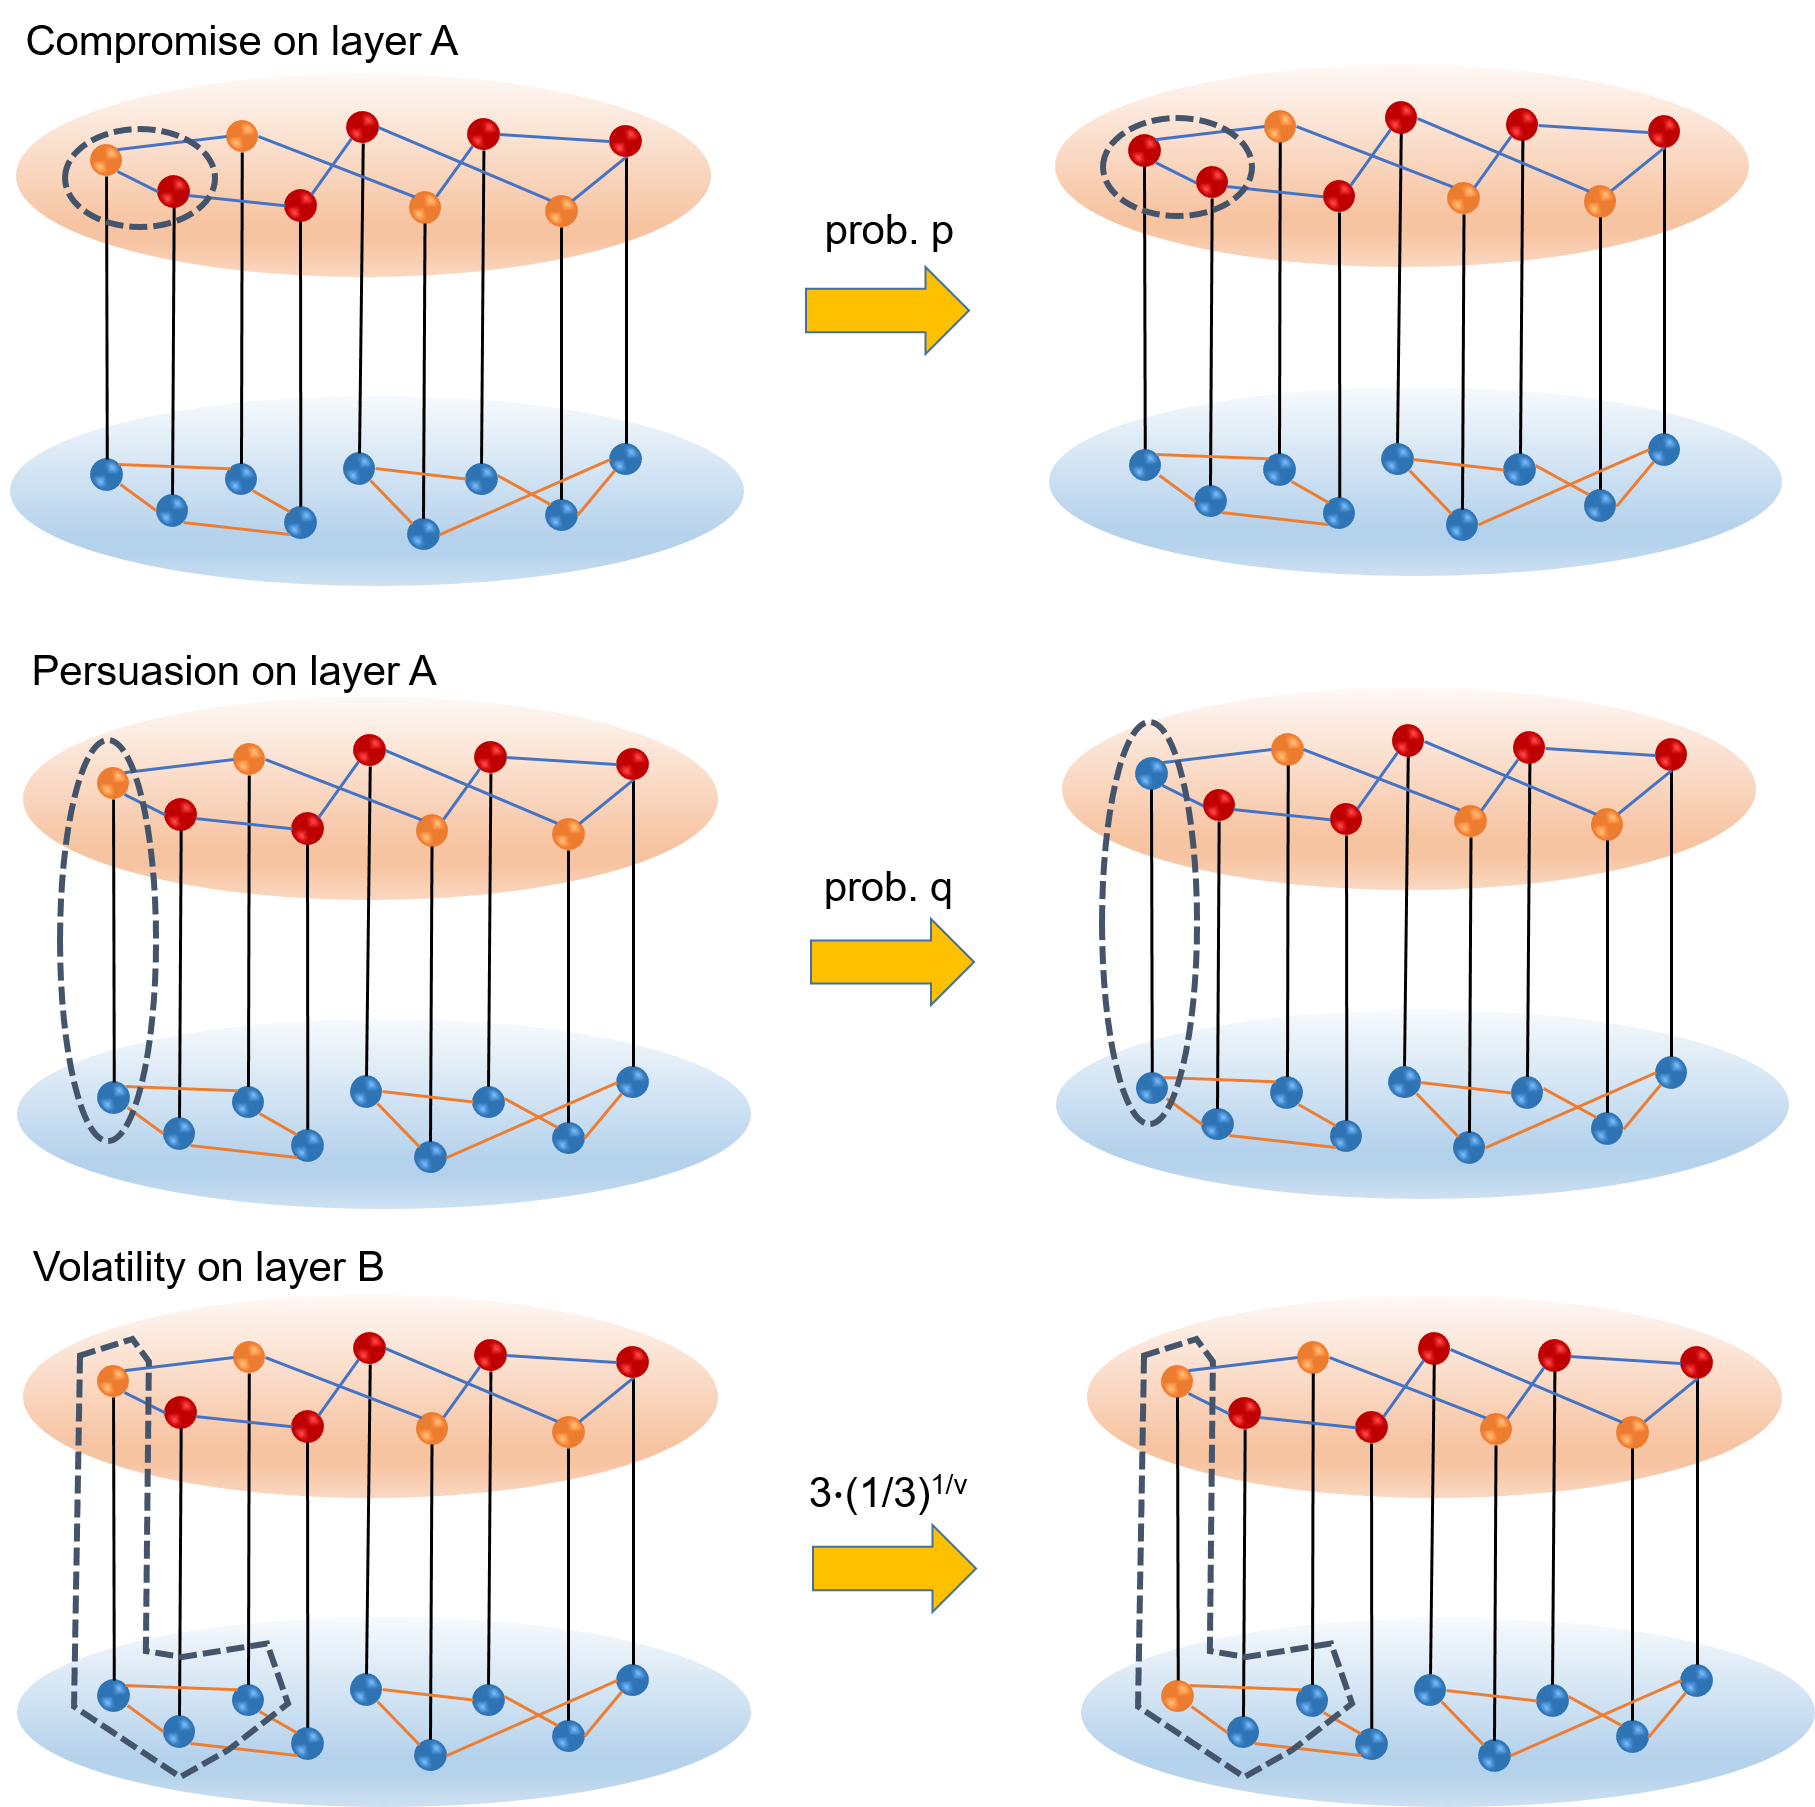
\includegraphics[width=\hsize]{chap2_dynamics.png}
	\caption{Dynamics on two layers}
	\label{chap2_dynamics}
\end{figure}

\section{Simulations and Analysis}
This model is nonlinear, and the applied dynamics are switched according to the states of nodes. In this model, practical mathematical tools can not be applied, and that precise analytical results are challenging to achieve.\parencite{nicolas2017, rainer2002}. For that reason, we analyze the above nonlinear model through a large number of simulations on the computer.

To start with a polarized competition, as the initial conditions,  nodes in layer A are all positive states, and nodes in layer B are all negative states, as shown in Fig.~\ref{chap2_modeling}. For nodes in layer A, it begins with the states where half of the nodes are $+1$, and the others are $+2$. The initial states of nodes in layer B have only $-1$.

There are two parameters, $p$ and $q$, in the dynamics of layer A. To represent the probability $p$ and probability $q$ together simply; we set $p+q=1$. So, $p$ represents the reinforcement or strength of opinion, such as extreme and moderate, which is scaled to be $0$ to $1$. And, there is only one parameter, $v$ in the dynamics of layer B. The scale of $v$ is also $0$ to $1$ as $p$. $v$ represents the volatility, which means how prone the state of a node can be changed into the opposite state.

In order to implement the interconnected dynamics, one step consists of two layers dynamics, where every node in layer A is checked with opinion dynamics, and every node in layer B updates its state according to the decision-making dynamics. The dynamics order follows updating the state of layer B after updating the state of layer A. The dynamics orders and updating rules of the two-layer network are explicitly discussed in chapter~\ref{chap4}.     

Each simulation takes $100$ steps for the opinion evolution, and $100$ simulations are considered for average results. To analyze the simulation results, we use \textit{`Average State'(AS)} to measure the average states of network and \textit{`Consensus Index'(CI)} to measure how close the state of the network is to consensus. The formulas follow as

\begin{equation}
AS = avg\left( {\sum\limits_i^{{K^A}} {S_i^A/4} } \right) + avg\left( {\sum\limits_i^{{K^B}} {S_i^B/2} } \right),
\end{equation}

\begin{equation}
CI = \frac{{({K_ + }^A \cdot {K_ - }^B) + ({K_ - }^A \cdot {K_ + }^B)}}{{{K^A} \cdot {K^B}}}.
\end{equation}

In these formulas, $S_i^A$ means the state of node $i$ in layer A, and $K^A$ is the number of nodes in layer A. ${K_ + }^A$ represents the number of nodes with the positive state in layer A.   

With \textit{AS}, it could be verified whether a consensus happens under the change of $p$ and $v$.  If a positive consensus happens, the \textit{AS} would be close to the value of $+1$. If a negative consensus happens, the \textit{AS} would be close to the value of $-1$. And, the medium values between $+1$ and $-1$ mean that the state of the network belongs to the coexistence or dissent part.

\begin{figure}[!htb]
	\centering
	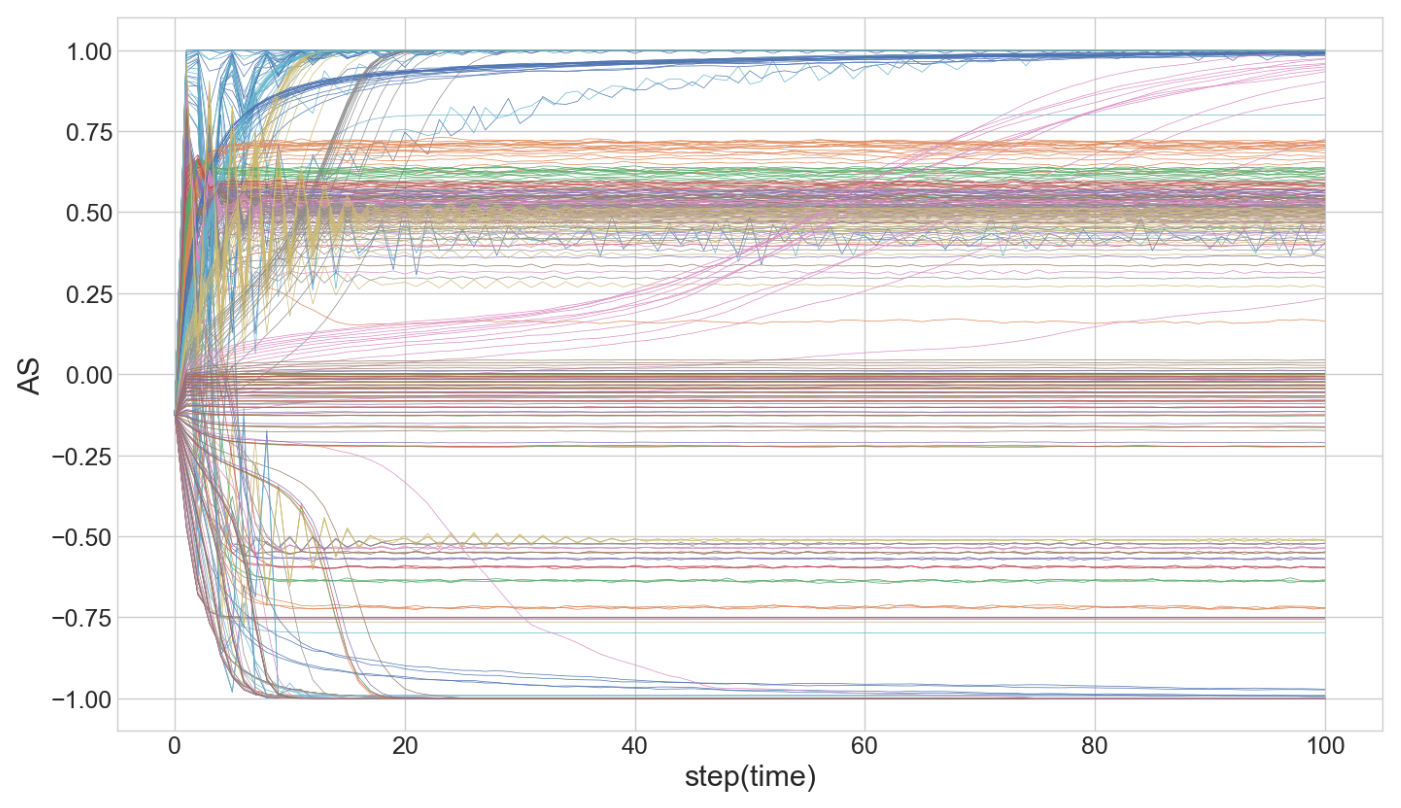
\includegraphics[width=\hsize]{chap2_timeflow_AS(BA3_BA3).png}
	\caption{AS values per each step according to all parameters}
	\label{chap2_timeflow_AS(BA3_BA3)}
\end{figure}

Fig.~\ref{chap2_timeflow_AS(BA3_BA3)} shows that \textit{AS} values are convergent to $+1$, $-1$, or other values as step(time) goes by. Reaching $+1$ means making a positive consensus, and reaching $-1$ means making a negative consensus. The other values mean a coexistence or dissent state. 

With \textit{CI}, it could be measured how close the state of the network is to consensus. If the \textit{CI} is close to $0$, the state of the network is close to a positive or negative consensus. If the \textit{CI} is close to $1$, a state of the network is a separated coexistence, where states of all nodes in layer A is opposed to states of all nodes in layer B. If the \textit{CI} is close to $0.5$, a state of the network is a mixed coexistence, where each layer has both positive and negative states of nodes.

\begin{figure}[!htb]
	\centering
	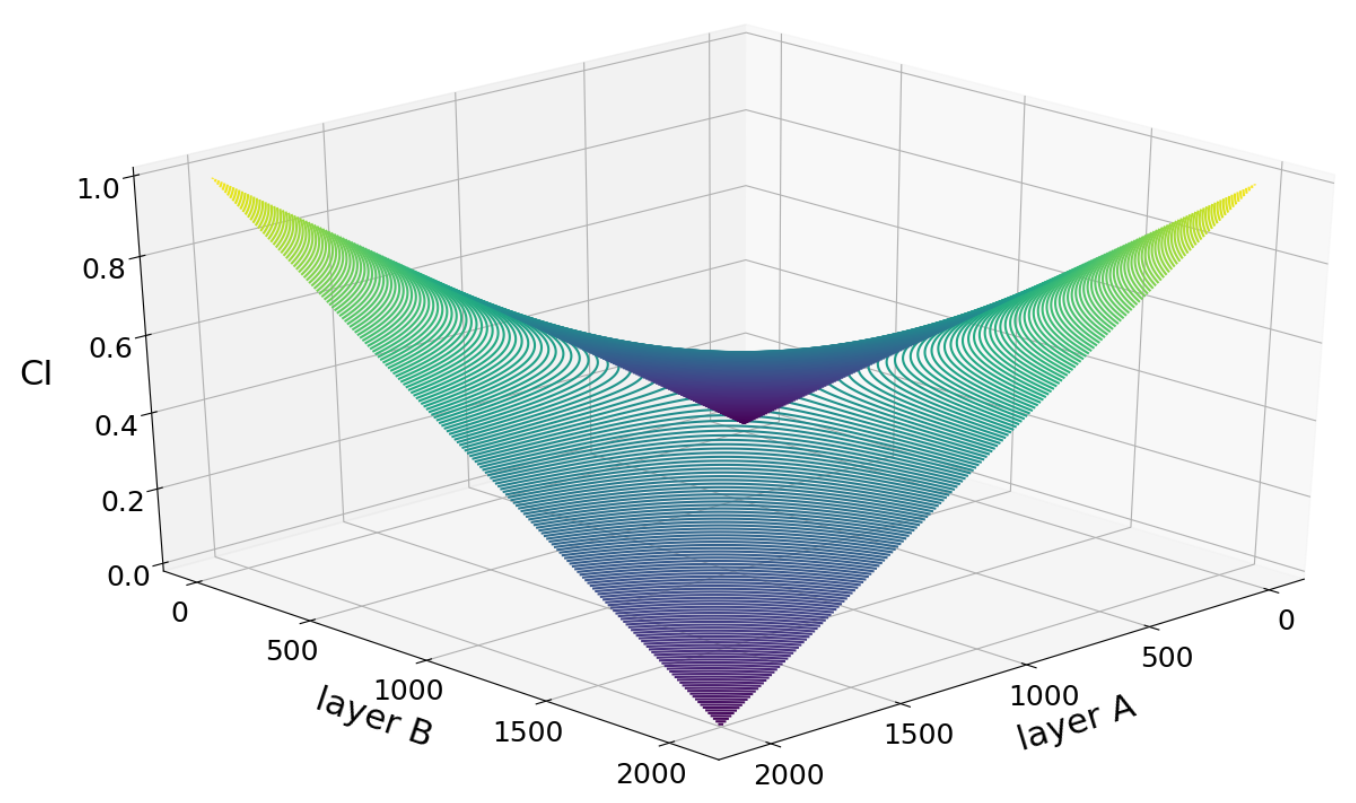
\includegraphics[width=\hsize]{chap2_CI_values.png}
	\caption{CI values according to all ${K_ + }^A$ and ${K_ + }^B$  }
	\label{chap2_CI_values}
\end{figure}

Fig.~\ref{chap2_CI_values} shows the characteristics of \textit{CI}. The same orientation states in two layers make \textit{CI} $0$. Opposite orientation states between two layers make \textit{CI} $1$. Moreover, mixed states in two layers make \textit{CI} close to $0.5$.

\begin{figure}[!htb]
	\centering
	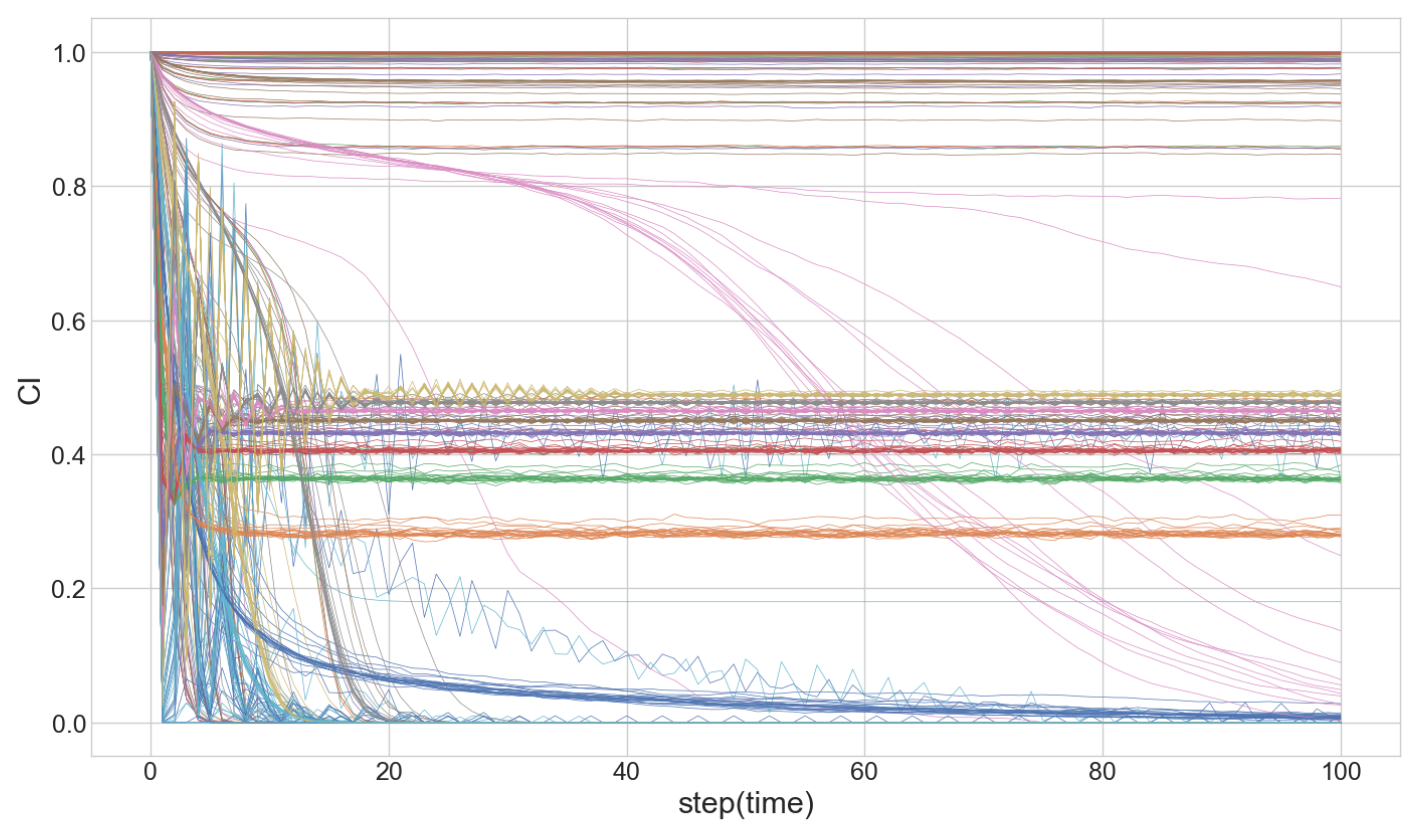
\includegraphics[width=\hsize]{chap2_timeflow_CI(BA3_BA3).png}
	\caption{CI values per each step according to all parameters}
	\label{chap2_timeflow_CI(BA3_BA3)}
\end{figure}

As Fig.~\ref{chap2_timeflow_CI(BA3_BA3)} shown, \textit{CI} values are convergent to $+1$, $0$, or other values as step(time) goes by. $0$ means positive or negative consensus of two-layer. $+1$ means separated opposite states of two-layers. The other values mean mixed states of two-layers. By using \textit{CI}, coexistence states can be divided into two categories, separated state and mixed state. 

To measure and evaluate the consensus results regarding two parameters $p$ and $v$, we use four kinds of indexes, including \textit{`AS total'}, \textit{`Positive Consensus Ratio'(PCR)}, \textit{`Negative Consensus ratio'(NCR)}, and \textit{`Consensus Ratio'(CR)}. \textit{AS total} means the summation of \textit{AS} for all $p$s and all $v$s. \textit{PCR} is the ratio of positive consensus over all simulations. Similarly, \textit{NCR} is the ratio of experiments with negative consensus. \textit{CR} is the ratio of experiments reaching consensus, i.e., the summation of \textit{PCR} and \textit{NCR}.

\begin{equation}
\begin{array}{cl}
AS\mbox{ \textit{total} } = \frac{{\sum\limits_j^m {\sum\limits_i^n {A{S_{{p _i},{v _j}}}} } }}{{n \times m }}, &
\begin{array}{l}
p  = \left\{ {{p _{\rm{1}}},{p _{\rm{2}}},\left. {\cdot\cdot\cdot,{p _n}} \right\}} \right.\\
v {\rm{ = }}\left\{ {{v _{\rm{1}}},{v _{\rm{2}}},\left. {\cdot\cdot\cdot,{v _m}} \right\}} \right.
\end{array}.\
\end{array}
\label{AS_total}
\end{equation}

In Eq(\ref{AS_total}), ${A{S_{{p _i},{v _j}}}}$ means $AS$ value according to parameters $p_i$ and $v_j$, which shows the total orientation and intensity of the interconnected network.

\begin{equation}
PCR = \frac{{\sum\limits_j^m {\sum\limits_i^n {(A{S_{{p _i},{v _j}}} \simeq  1)} } }}{{n \times m}}.
\label{PCR}
\end{equation}

In Eq(\ref{PCR}),  ${A{S_{{p _i},{v _j}}} \simeq  1}$ means positive consensus.

\begin{equation}
NCR = \frac{{\sum\limits_j^m {\sum\limits_i^n {(A{S_{{p _i},{v _j}}} \simeq   - 1)} } }}{{n \times m}}.
\label{NCR}
\end{equation}

In Eq(\ref{NCR}), ${A{S_{{p _i},{v _j}}} \simeq  -1}$ means negative consensus.


\begin{figure}[!htb]
	\centering
	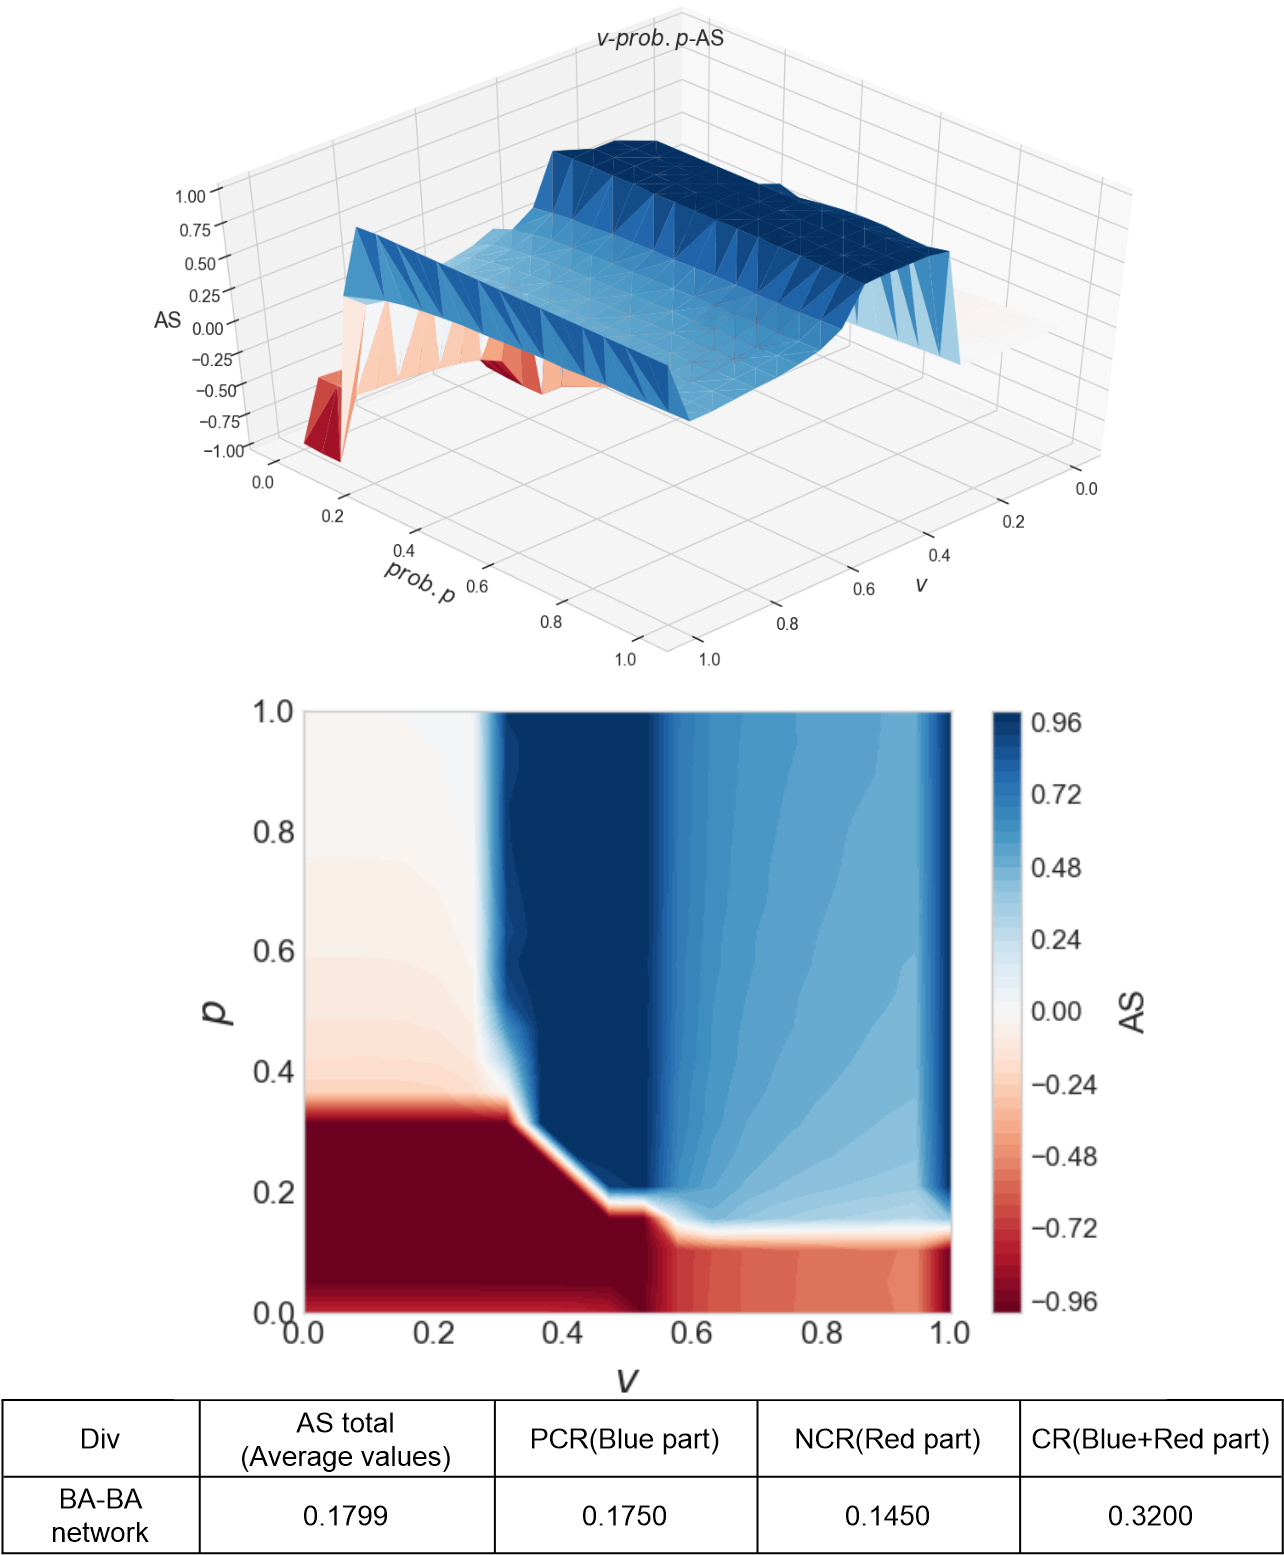
\includegraphics[width=\hsize]{chap2_AS_total(BA3_BA3).png}
	\caption{The example of simulation : BA-BA network}
	\label{chap2_AS_total(BA3_BA3)}
\end{figure}

Fig.~\ref{chap2_AS_total(BA3_BA3)} shows the states of the interconnected network according to all $p$s and all $v$s. The $X$-axis is the $p$, the $Y$-axis is the $v$, and the $Z$-axis represents \textit{AS}. The closer the color is to blue color, the more it has a positive consensus. Moreover, the closer the color is to red color, the more it has a negative consensus. Light-colored and white areas have coexistence with both positive states and negative states. Here, we can measure the consensus by using indexes, \textit{`AS total'}, \textit{`PCR'}, \textit{`NCR'}, and \textit{`CR'}. The average value of this figure means \textit{`AS total'}. The blue part area means \textit{`PCR'}, the red part area means \textit{`NCR'}, and the summation of both\textit{`PCR'} and \textit{`NCR'} means \textit{`CR'}. \\



    

%# -*- coding: utf-8-unix -*-
% !TEX program = xelatex
% !TEX root = ../thesis.tex
% !TEX encoding = UTF-8 Unicode
%%==================================================
%% chapter02.tex for SJTU Master Thesis
%% based on CASthesis
%% modified by wei.jianwen@gmail.com
%% Encoding: UTF-8
%%==================================================


\chapter{Competition on two layer with networks of various structures}
\label{chap:competition on two layer with networks of various structures}
In this chapter, based on the competition model described in chapter.\ref{chap:modeling and analysis methods}, simulations would be implemented with changing the network structures. As the basic model, interconnected layer with random regular networks would be provided. And then, the structure of interconnected network  would be altered by changing the internal edges, external edges and network types. Finally, all simulations would be compared and analyzed with the indexes, \textit{AS total}, \textit{PCR}, \textit{NCR} and \textit{CR}

\section{Competition on Random Regular Networks}
\label{competition on Random Regular Networks}
\begin{figure}[!h]
	\centering
	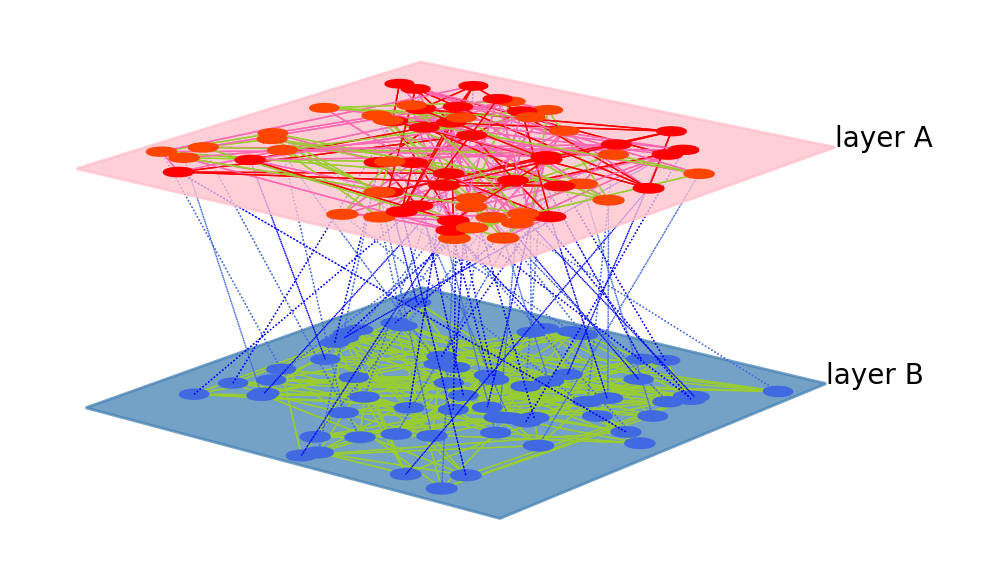
\includegraphics[width=\hsize]{chap3_RR(5)_RR(5).png}
	\caption{Competition on random regular network}
	\label{chap3_RR(5)_RR(5)}
\end{figure}
\begin{figure}[!h]
	\centering
	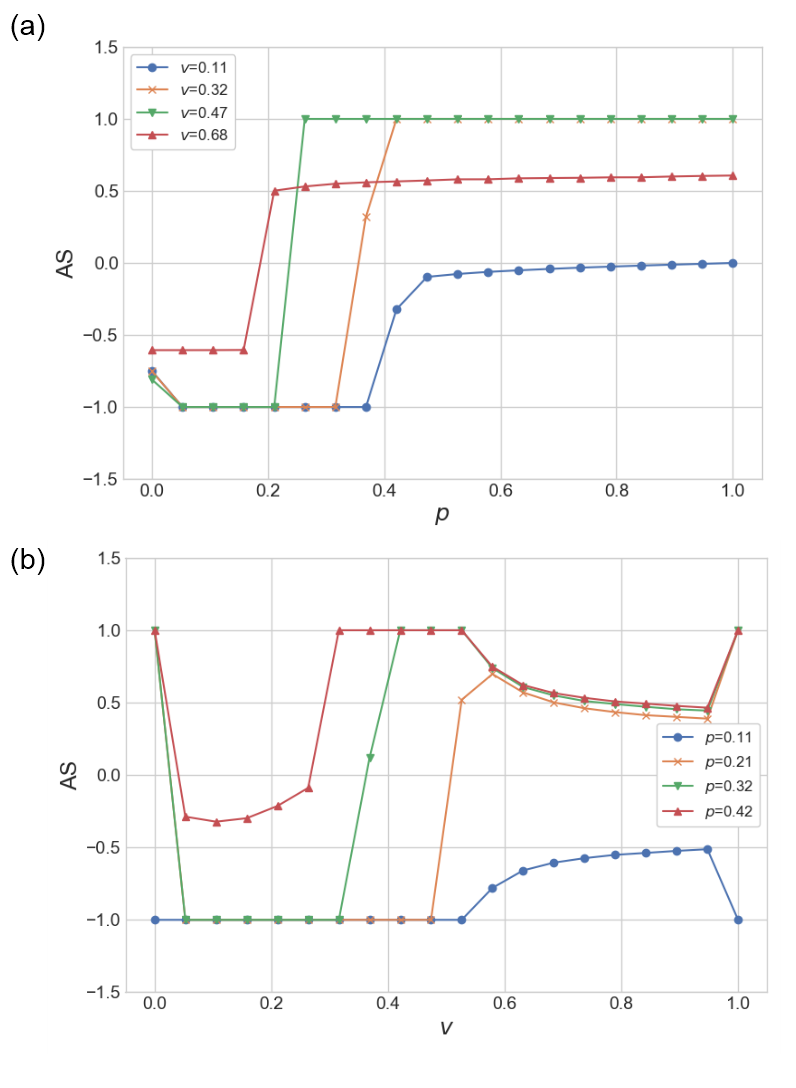
\includegraphics[width=\hsize]{chap3_RR(5)_RR(5)_2d.png}
	\caption{(a) $p$-\textit{AS} chart according to certain $v$ values. (b) $v$-\textit{AS} chart according to certain $p$ values.}
	\label{chap3_RR(5)_RR(5)_2d}
\end{figure}
\begin{figure}[!h]
	\centering
	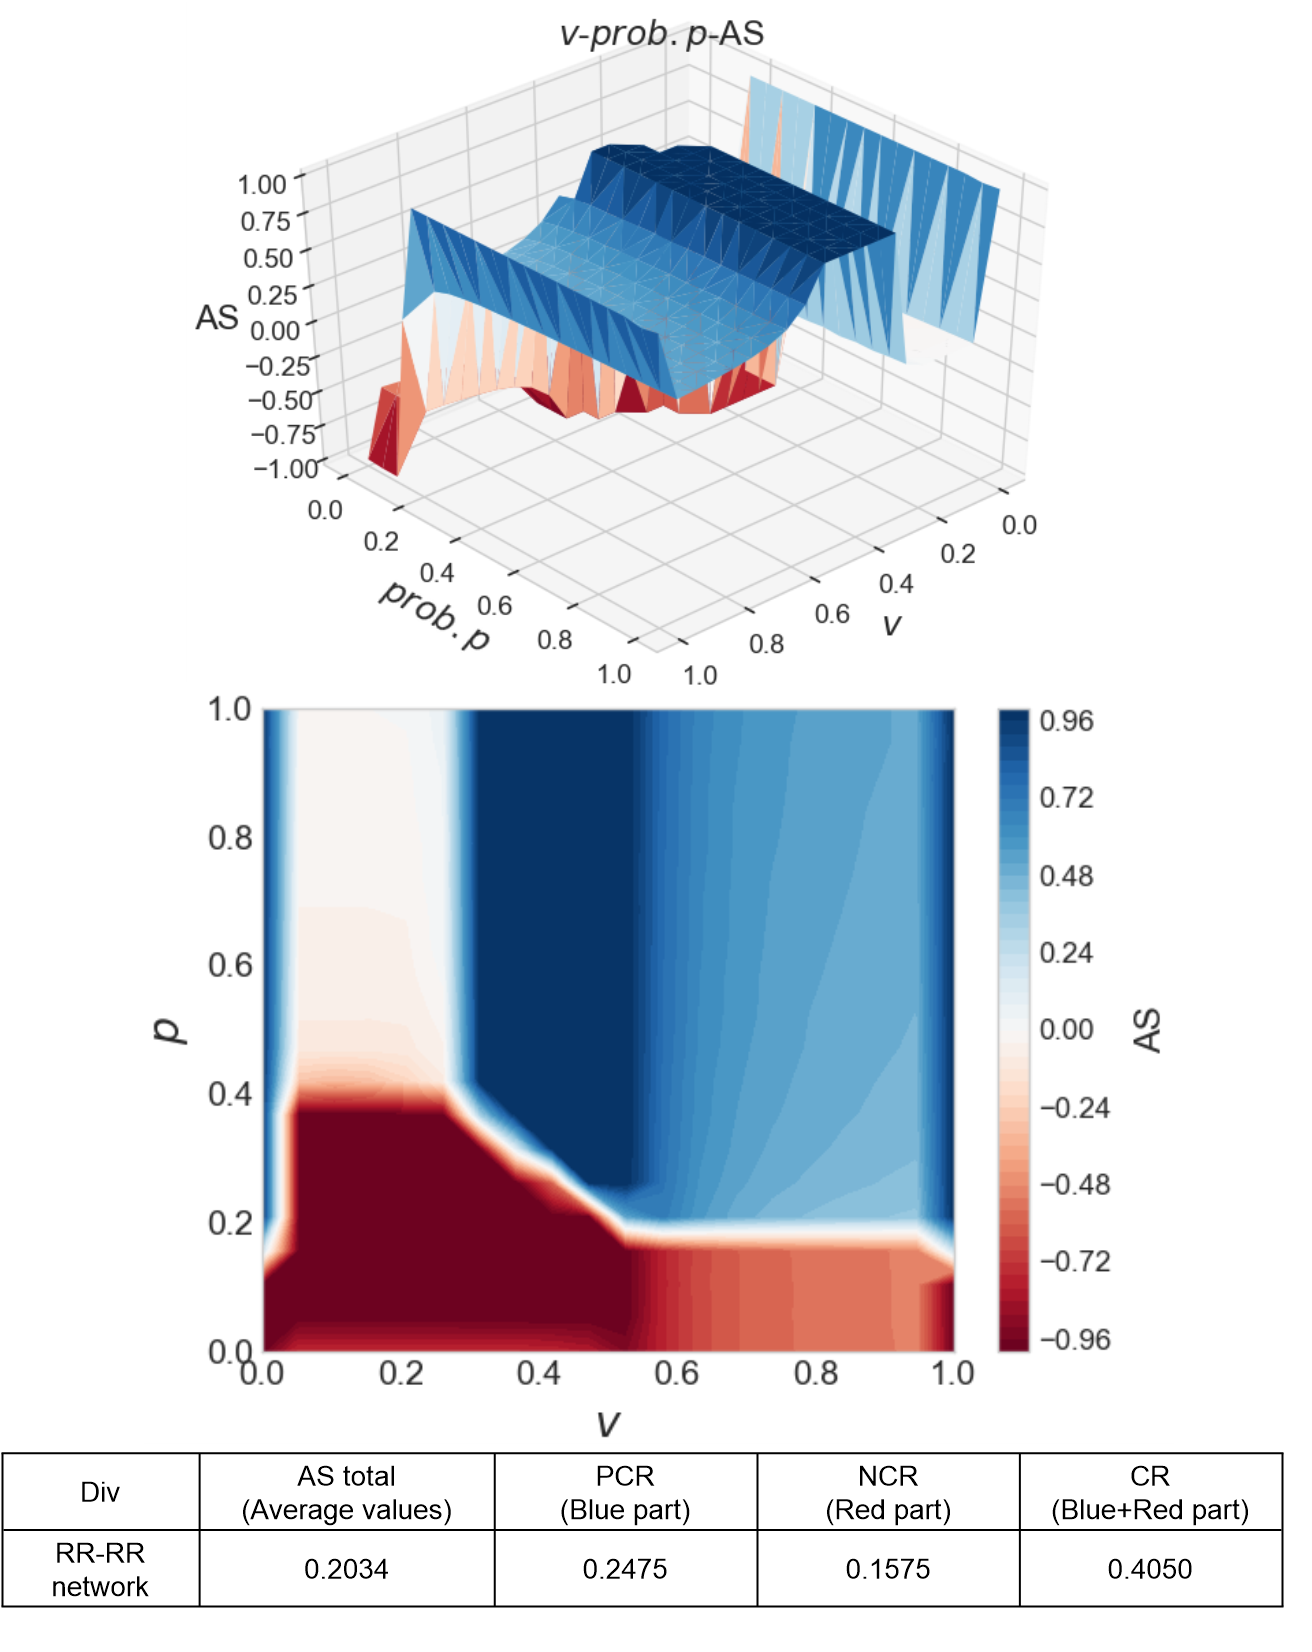
\includegraphics[width=\hsize]{chap3_RR(5)_RR(5)_total.png}
	\caption{\textit{AS} with changing with all $p$ and $v$}
	\label{chap3_RR(5)_RR(5)_total}
\end{figure}
In this section, simulation results on random regular network would be provided to comprehend the competition of two layers. Each layer consists of random regular network that has $N$ nodes with $k$ internal edges as introduced in \parencite{kimsangwoo2012, choi2011, bela2001}. Each node of one layer is connected with a random node on the other layer. This means each node has only $1$ external un-directed edge. Simulations are performed on network with $N=2048$, and $k = 5$. 

The simulation results are shown in Fig.~\ref{chap3_RR(5)_RR(5)_2d} and Fig.~\ref{chap3_RR(5)_RR(5)_total}.  Fig.~\ref{chap3_RR(5)_RR(5)_2d} presents that how the `Average State'(\textit{AS}) are changed according to the other parameter($v$ or $p$), when one parameter($p$ or $v$) is constant. So we can know that how each parameter works on the network. Fig.~\ref{chap3_RR(5)_RR(5)_total} provides total results with all parameters. Through these figures, the characteristics of network would be analyzed.

Fig.~\ref{chap3_RR(5)_RR(5)_2d}(a) shows that when $p > 0.2$, $0.32 < v < 0.47$, it normally tends to positive consensus. Here, we could found out that if $v$ is lower or larger than certain values, it doesn't make consensus. In Fig.~\ref{chap3_RR(5)_RR(5)_2d}(b), as $v$ increases, it normally change from negative to positive consensus. But, it is found out that when $p$ is very low($p \le 0.11$), it doesn't make positive consensus.  To sum up, when $p$ is large enough, it tends to make positive consensus. But, when $v$ is small enough, it tends to be changed into negative consensus.

Fig.~\ref{chap3_RR(5)_RR(5)_total} shows the states of two layers according to all $p$s and all $v$s. As previously described in chapter.~\ref{chap:modeling and analysis methods}, blue area is for positive consensus, red area is for negative consensus, and light colored and white area is for coexistence. And indexes for consensus are also measured. Positive consensus area is $0.2475$, and negative consensus area is $0.1575$. Coexistence area is $1 - CR = 0.5950$. By using these values and figures, this model would be compared with networks of various structures in next section. Through these figures, the characteristics of parameters can be arranged. First, large $p$ tends to make positive consensus and small $p$ tends to make negative consensus. Second, small $v$ tends to make negative consensus, and large $v$ tends to make coexistence state. 

\section{Competition on Networks with different number of external links}
\begin{figure}[!htb]
	\centering
	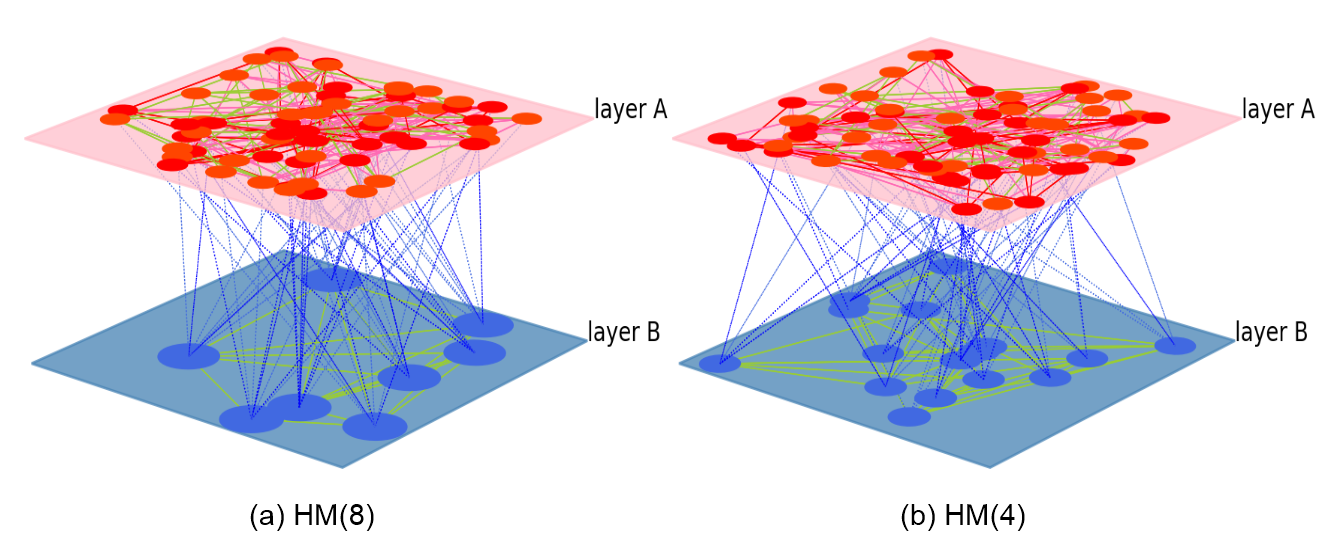
\includegraphics[width=\hsize]{chap3_HM.png}
	\caption{Competition on hierarchical model}
	\label{chap3_HM}
\end{figure}
In this section, we consider the influence of external links. Based on \textit{RR-RR} model in section~\ref{competition on Random Regular Networks}, we reduce the number of nodes in layer B at a certain rate and increase the external links from nodes in layer B accordingly as shown in Fig.~\ref{chap3_HM}.  We denote \textit{HM(n)} as a hierarchical model with a level $n$, which means that the number of nodes in layer B is $1/n$ of the number of nodes in layer A, and the number of external links from node in layer B is $n$ in view that the number of external links from node in layer A is $1$. In other words, each node in layer A has one external edge, but each node in layer B has $n$ external edges for \textit{HM(n)}, which means one node in layer B can interact with $n$ nodes in layer A.
\begin{figure}[!htb]
	\centering
	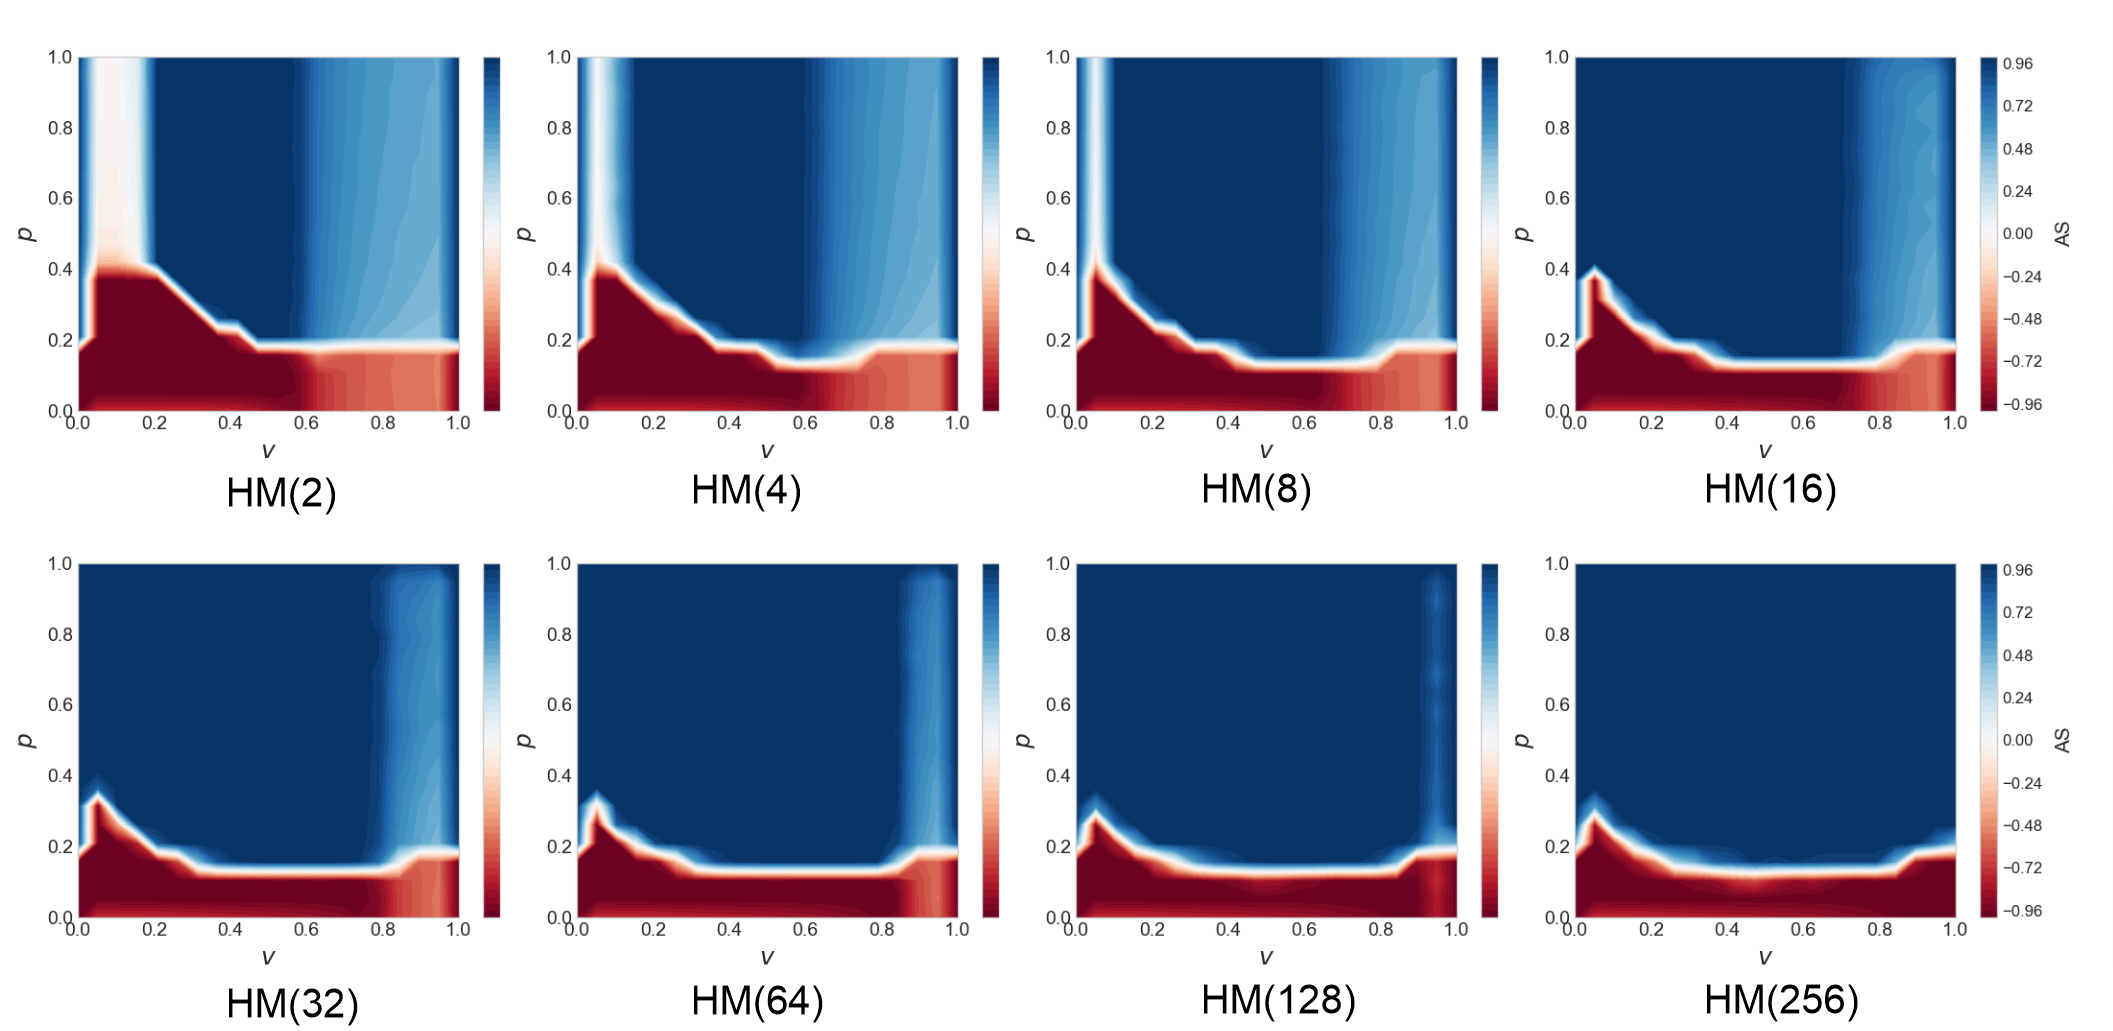
\includegraphics[width=\hsize]{chap3_HMs_AStotal.png}
	\caption{\textit{AS total} on various hierarchical models}
	\label{chap3_HMs_AStotal}
\end{figure}
To find out the significant influence of external edges, various \textit{HM(n)s} were simulated.  Totally, $8$ \textit{HM(n)}s, \textit{HM(2), HM(4), HM(8), HM(16), HM(32), HM(64), HM(128), HM(256)} were arranged as shown in Fig.~\ref{chap3_HMs_AStotal}.  
Fig.~\ref{chap3_HMs_AStotal} shows that \textit{HM(2)} has the most area for coexistence part(light colored and white area) and \textit{HM(256)} has the most are for consensus part(blue and red area). As $n$ in \textit{HM(n)} is increased, coexistence area is decreased and consensus area is increased. Particularly, positive consensus area is significantly increased, negative consensus area is slightly decreased.  
\begin{figure}[!htb]
	\centering
	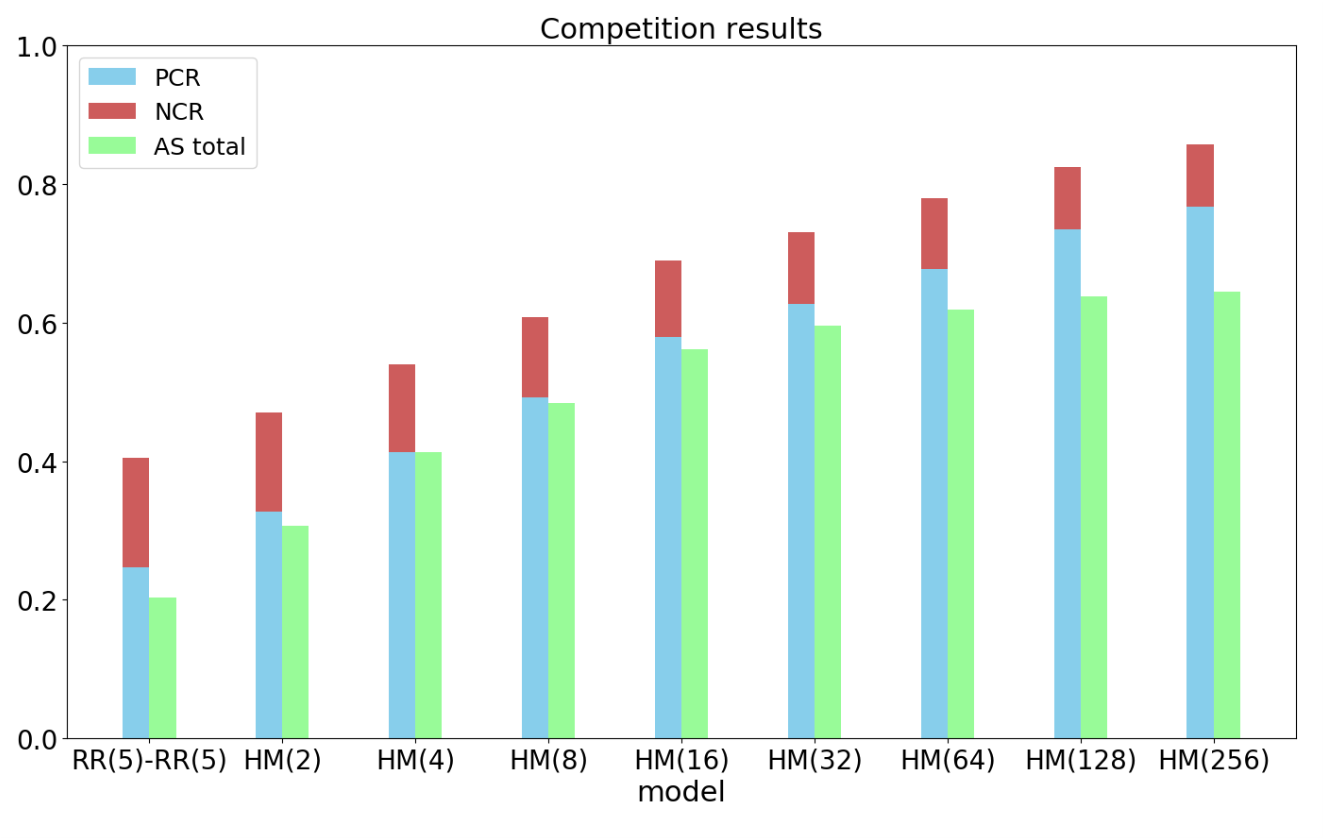
\includegraphics[width=\hsize]{chap3_HMs_total.png}
	\caption{Histogram for \textit{PCR, NCR, AS total} of Hierarchical Models(\textit{HM(n)})}
	\label{chap3_HMs_total}
\end{figure}
To clearly find out the difference between models, we use the indexes, \textit{PCR, NCR, AS total}. Fig.~\ref{chap3_HMs_total} shows the results to analyze \textit{HM(n)} with indexes. Blue color bar is for \text{PCR}, red color bar is for \text{NCR}, and green color bar is for \text{AS total}. Comparing \textit{HMs} with \textit{Basic model(RR(5)-RR(5))}, \textit{CR} \textit{PCR} and \textit{AS total} are all increased remarkably. \textit{HMs} have more positive consensus part than \textit{RR(5)-RR(5)}. And, \textit{HMs} have less negative consensus part than \textit{RR(5)-RR(5)}. It shows that as the number of B nodes are decreased, it is easy to make positive consensus(layer A opinion) and hard to make negative consensus(layer B opinion).  

In summary, all the Hierarchical Models have more consensus ratio than \textit{Random Regular Networks} Model. However, positive consensus ratio is increased, but negative consensus ratio is decreased. It is found out that as the number of B nodes are more decreased, it makes easier to make positive consensus and harder to make negative consensus. In real world, it would be analyzed that as the number of leaders is less, social conflict are decreased and the opinion is convergent to social opinion(layer A). But, sometimes there are some dangers to ignore the leader opinions(layer B), or to cause more social conflict when there are stubborn leaders, that would be simulated in chapter.\ref{chap:finding key nodes on two layer networks}. 

\section{Competition on Networks with different number of internal links}
\begin{figure}[!htb]
	\centering
	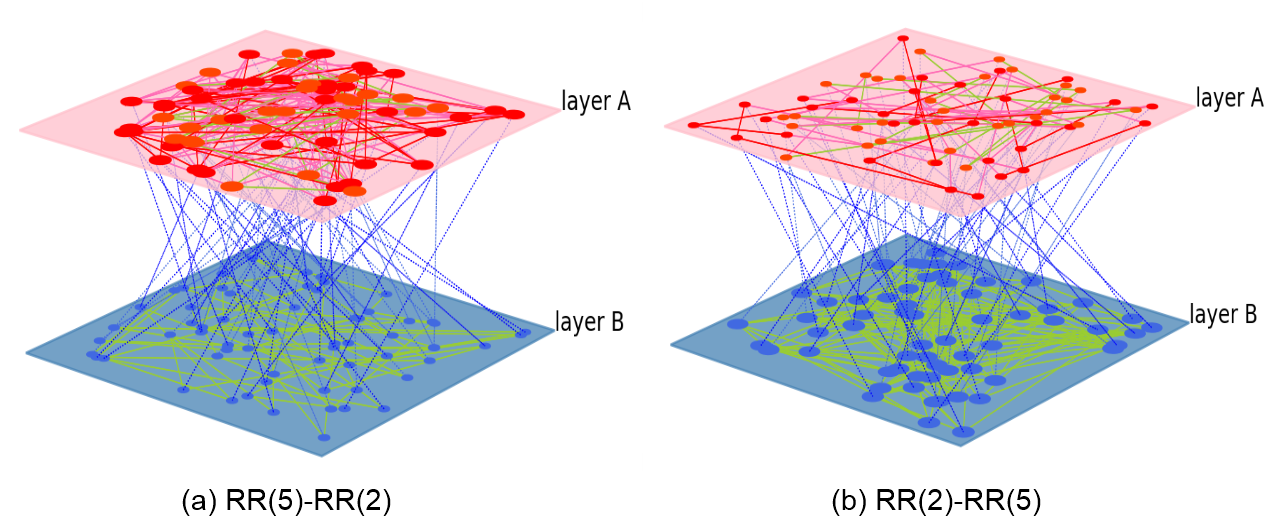
\includegraphics[width=\hsize]{chap3_changing_internal_edges.png}
	\caption{Competition on interconnected networks with different internal edges}
	\label{chap3_changing_internal_edges}
\end{figure}
Next, the interconnected networks are simulated with various internal degrees in order to define and evaluate the influence of internal degrees. Random regular network would be applied and the number of internal degrees on each node is switched to various numbers as shown in Fig.~\ref{chap3_changing_internal_edges}. But, there is no change on external degree, which would be fixed to only $1$. Here, \textit{RR(n)-RR(m)} represents layer A has random regular network with $n$ internal edges per a node, layer B has random regular network with $m$ internal edges per a node.
\begin{figure}[!htb]
	\centering
	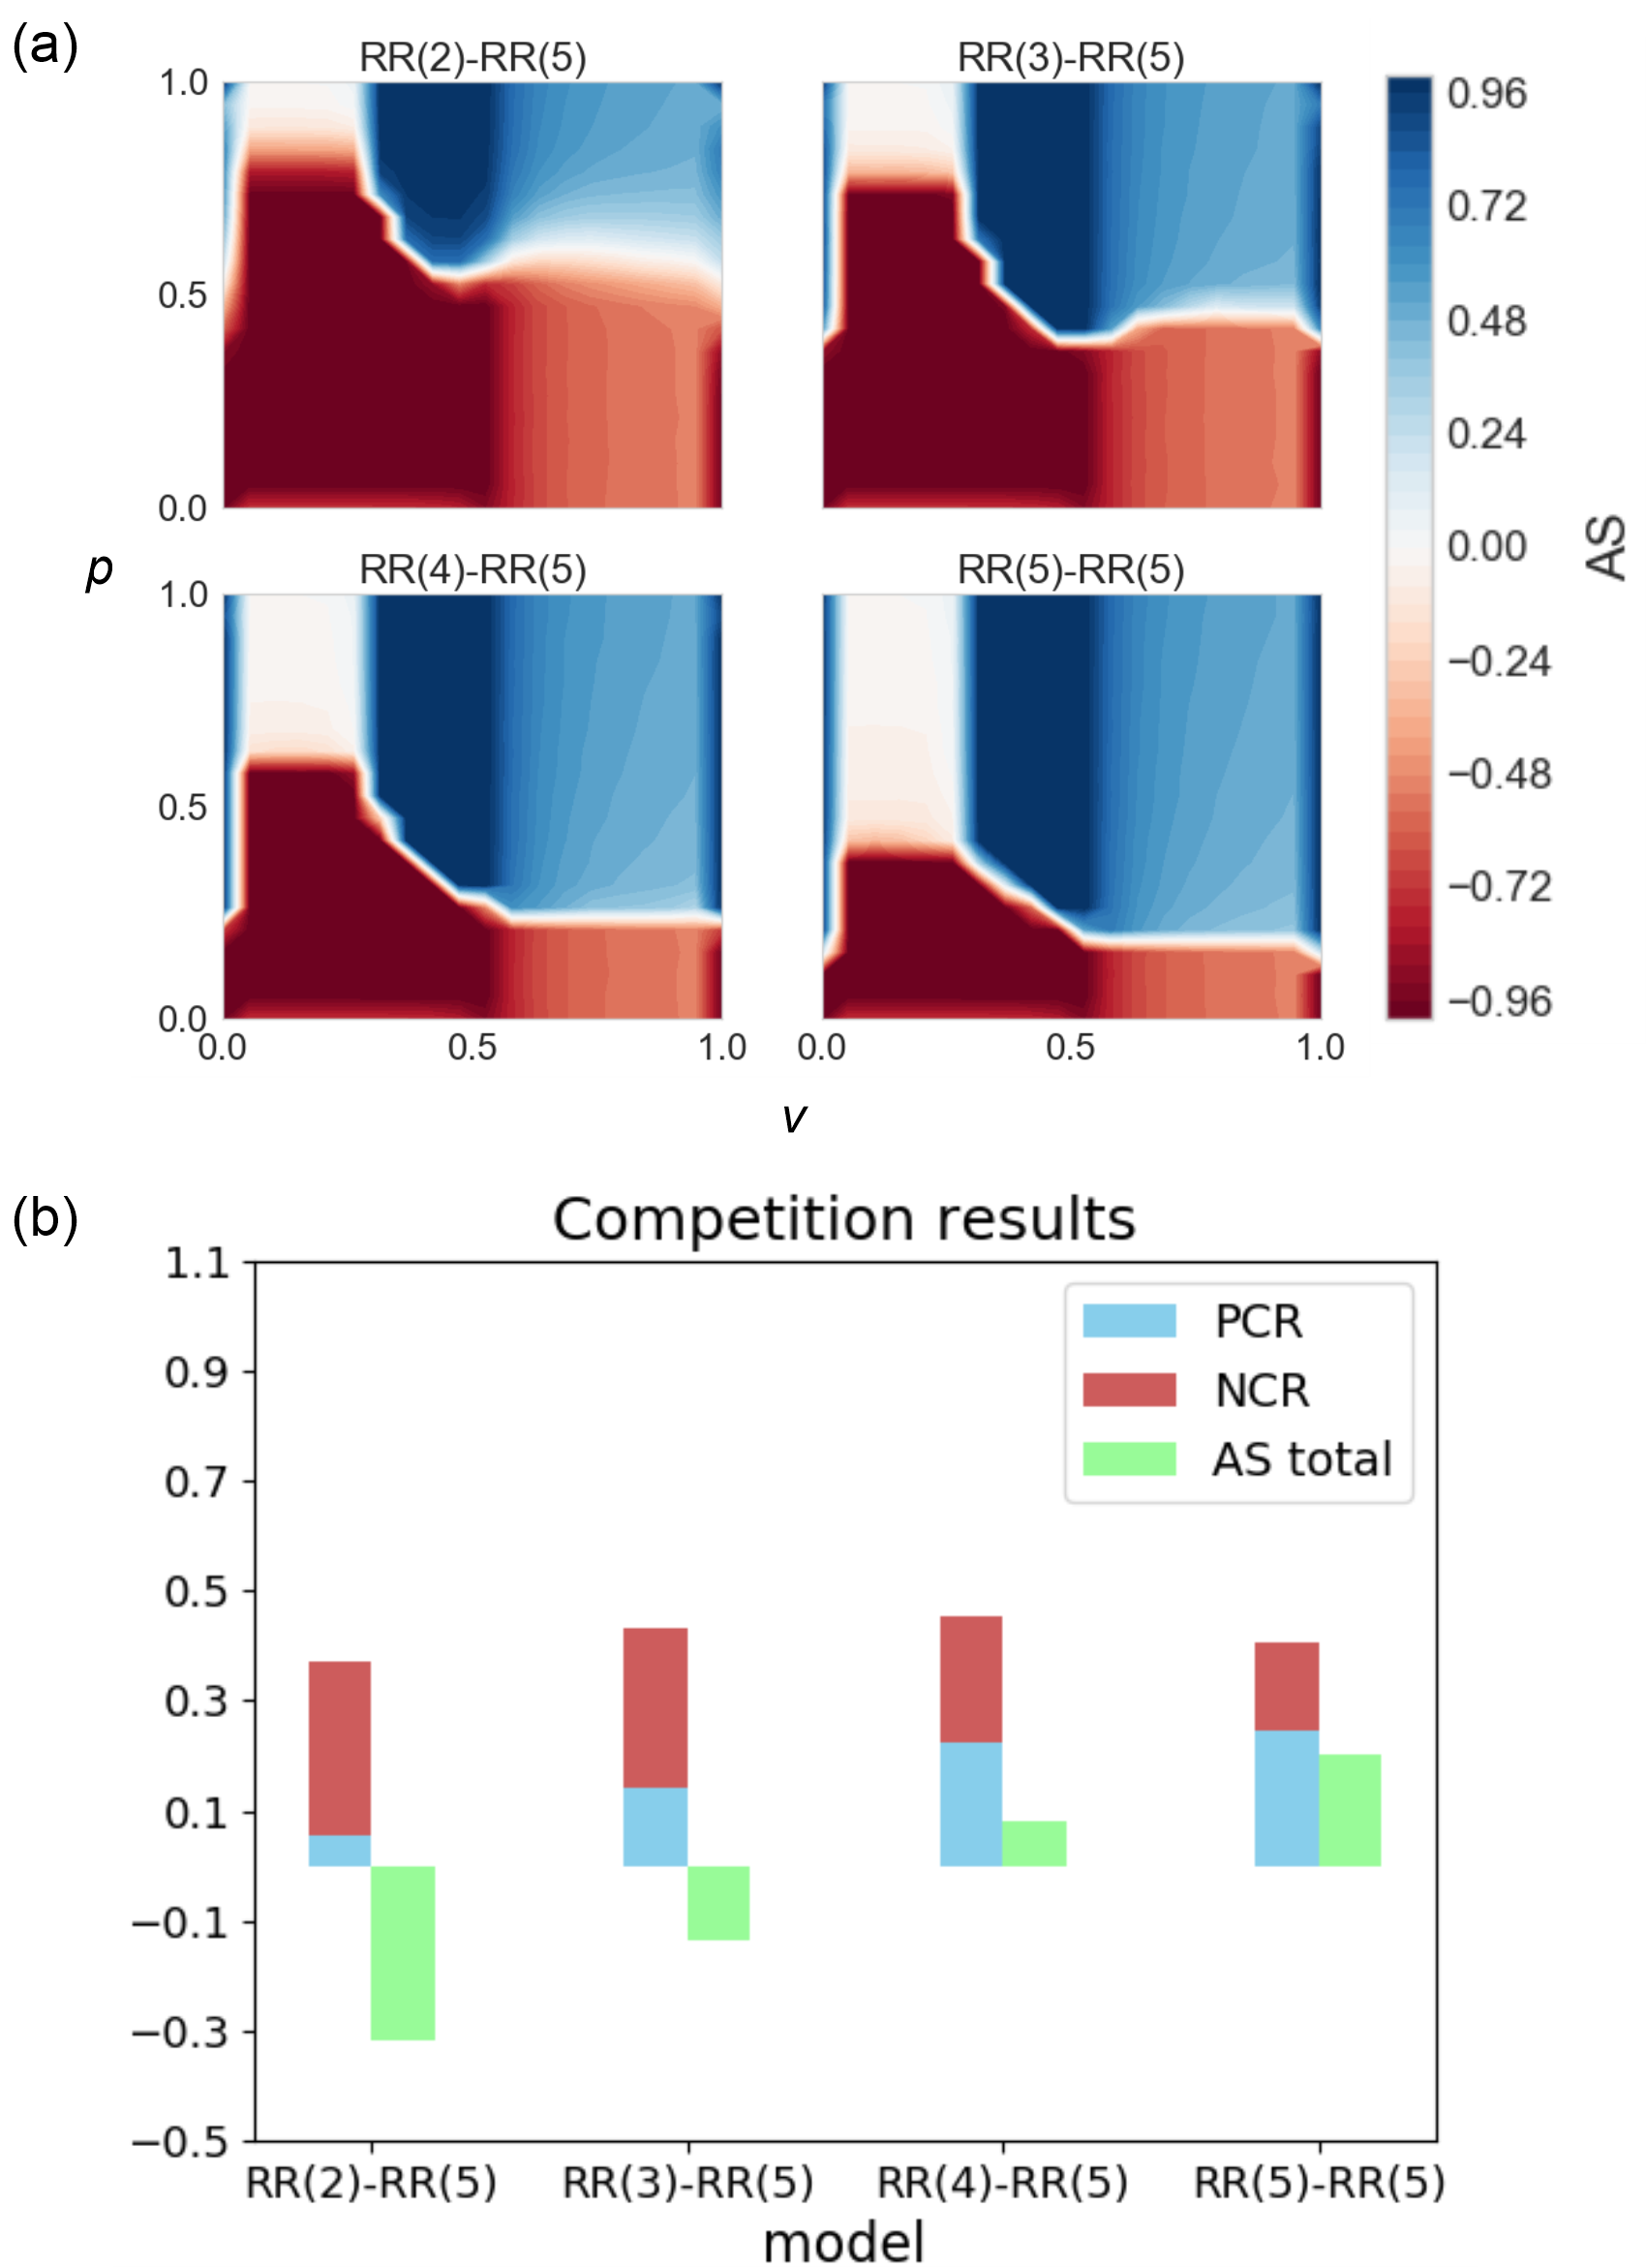
\includegraphics[width=\hsize]{chap3_internal_edge_A_total1.png}
	\caption{Simulation results with different internal degrees on layer A}
	\label{chap3_internal_edge_A_total}
\end{figure}
First, the internal degrees on layer A are changed. The internal degrees on layer B are fixed to $5,120$, which means each node has $5$ internal degrees on layer B, and the internal degrees on layer A are switched into $2,048$, $3,072$, $4,096$, or $5,120$, which means each node has $2$, $3$, $4$, or $5$ internal degrees on layer A. Fig.~\ref{chap3_internal_edge_A_total} shows the simulation results for changing the internal degrees on layer A. As shows in Fig.~\ref{chap3_internal_edge_A_total} (a), as the number of internal degrees on layer A is increased, the red part is decreased and the blue part is increased.  

To clearly compare and analyze the results, the results are presented with the indexes, \textit{PCR, NCR, AS total} in Fig.~\ref{chap3_internal_edge_A_total} (b), which shows that as the number of internal degrees on layer A is increased, negative consensus is decreased and positive consensus is increased. As shown in Fig.~\ref{chap3_internal_edge_A_total}, RR(5)-RR(5) has the most \textit{PCR}, and RR(2)-RR(5) has the most \text{NCR}. However, all models in Fig.~\ref{chap3_interal_edge_A_total} have almost same \textit{CR}. It can be analyzed that the number of internal degrees on layer A has the tendency to keep positive state and to change negative state into positive state. 
\begin{figure}[!htb]
	\centering
	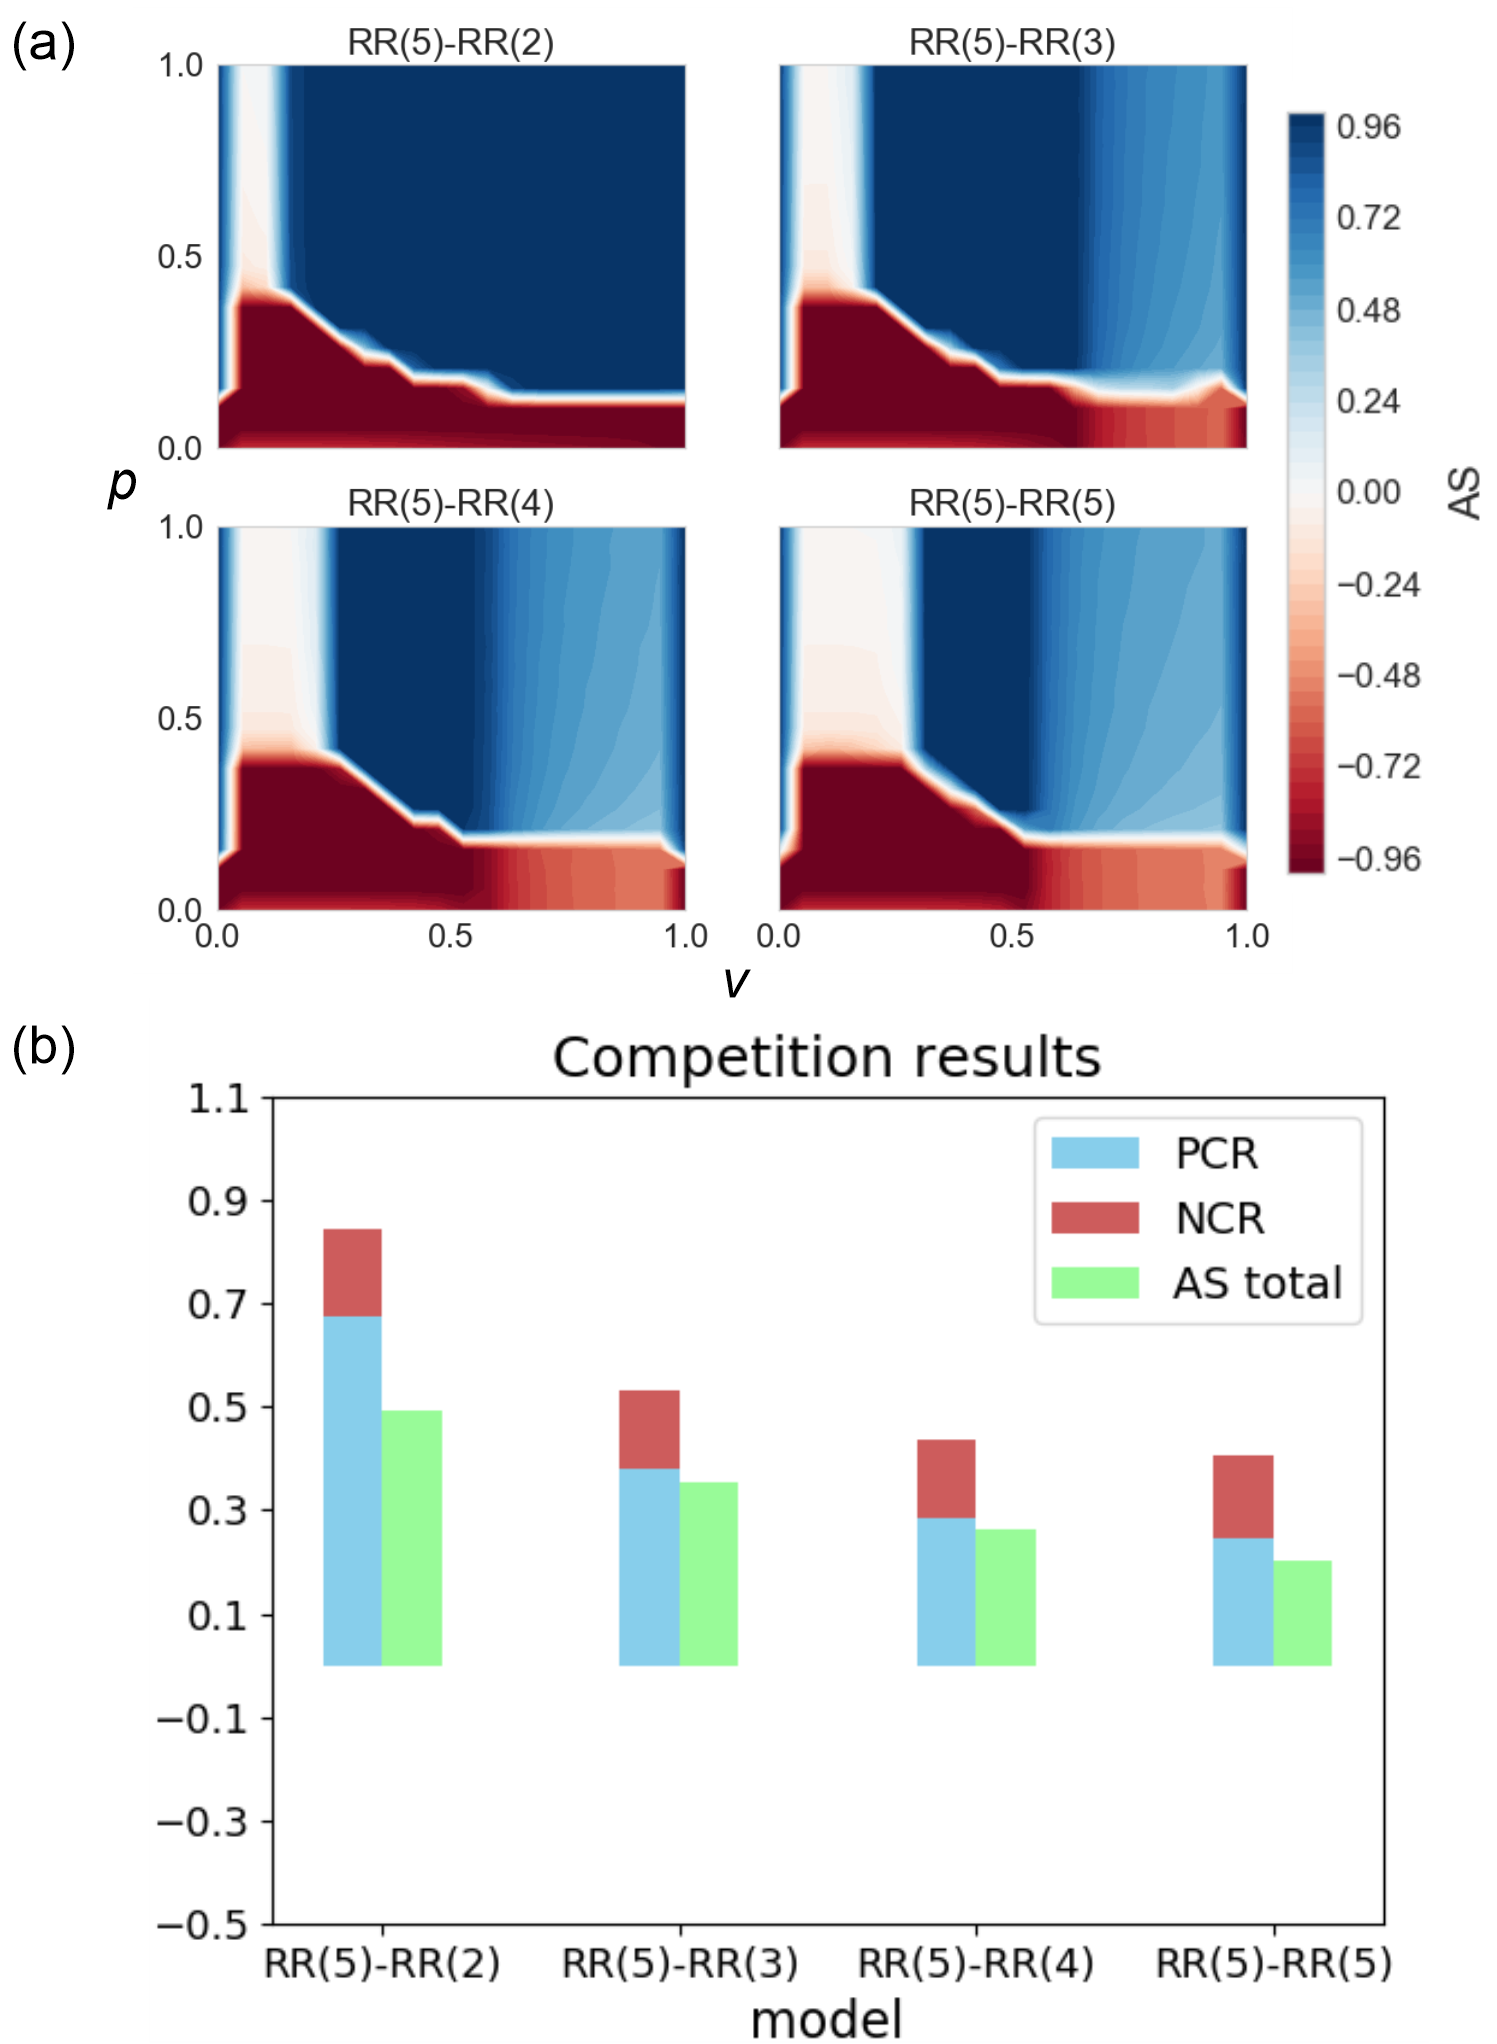
\includegraphics[width=\hsize]{chap3_internal_edge_B_total1.png}
	\caption{Simulation results with different internal degrees on layer B}
	\label{chap3_internal_edge_B_total}
\end{figure}
Next, the internal degrees on layer B are changed. The internal degrees on layer A are fixed to  $5,120$, which means each node has $5$ internal degrees on layer A, and the internal degrees on layer B are switched into $2,048$, $3,072$, $4,096$, or $5,120$, which means each node has $2$, $3$, $4$, or $5$ internal degrees on layer B.  
Fig.~\ref{chap3_internal_edge_B_total} shows the simulation results with changing the number of internal degrees on layer B. As shows in Fig.~\ref{chap3_internal_edge_B} (a), as the number of internal degrees on layer B is increased, the blue part is decreased, the white and light color part is increased, and the red part is almost same, though the shape of red area is changed.  As shown in Fig.~\ref{chap3_internal_edge_B_total} (b), RR(5)-RR(2) has the most \textit{PCR} and \textit{CR}, and RR(5)-RR(5) has the least \text{PCR} and \textit{CR}. However, all models in Fig.~\ref{chap3_interal_edge_B_total} have almost same \textit{NCR}. It can be analyzed that the number of internal degrees on layer B has the tendency to hinder positive consensus state and has the inverse relation with \textit{CR}. As the number of internal degrees on layer B is increased, \textit{PCR} and \textit{CR} is inversely decreased.\\ 
Considering two cases where internal degree of layer A is changed and where internal degree of layer B is changed, it is recognized that the role of internal degrees on layer A is different with internal degrees on layer B. The internal degrees on layer A has the function to keep the state of layer A, and the internal degrees on layer B has the function to restrain the consensus state of layer A and make coexistence part. 
\begin{figure}[!htb]
	\centering
	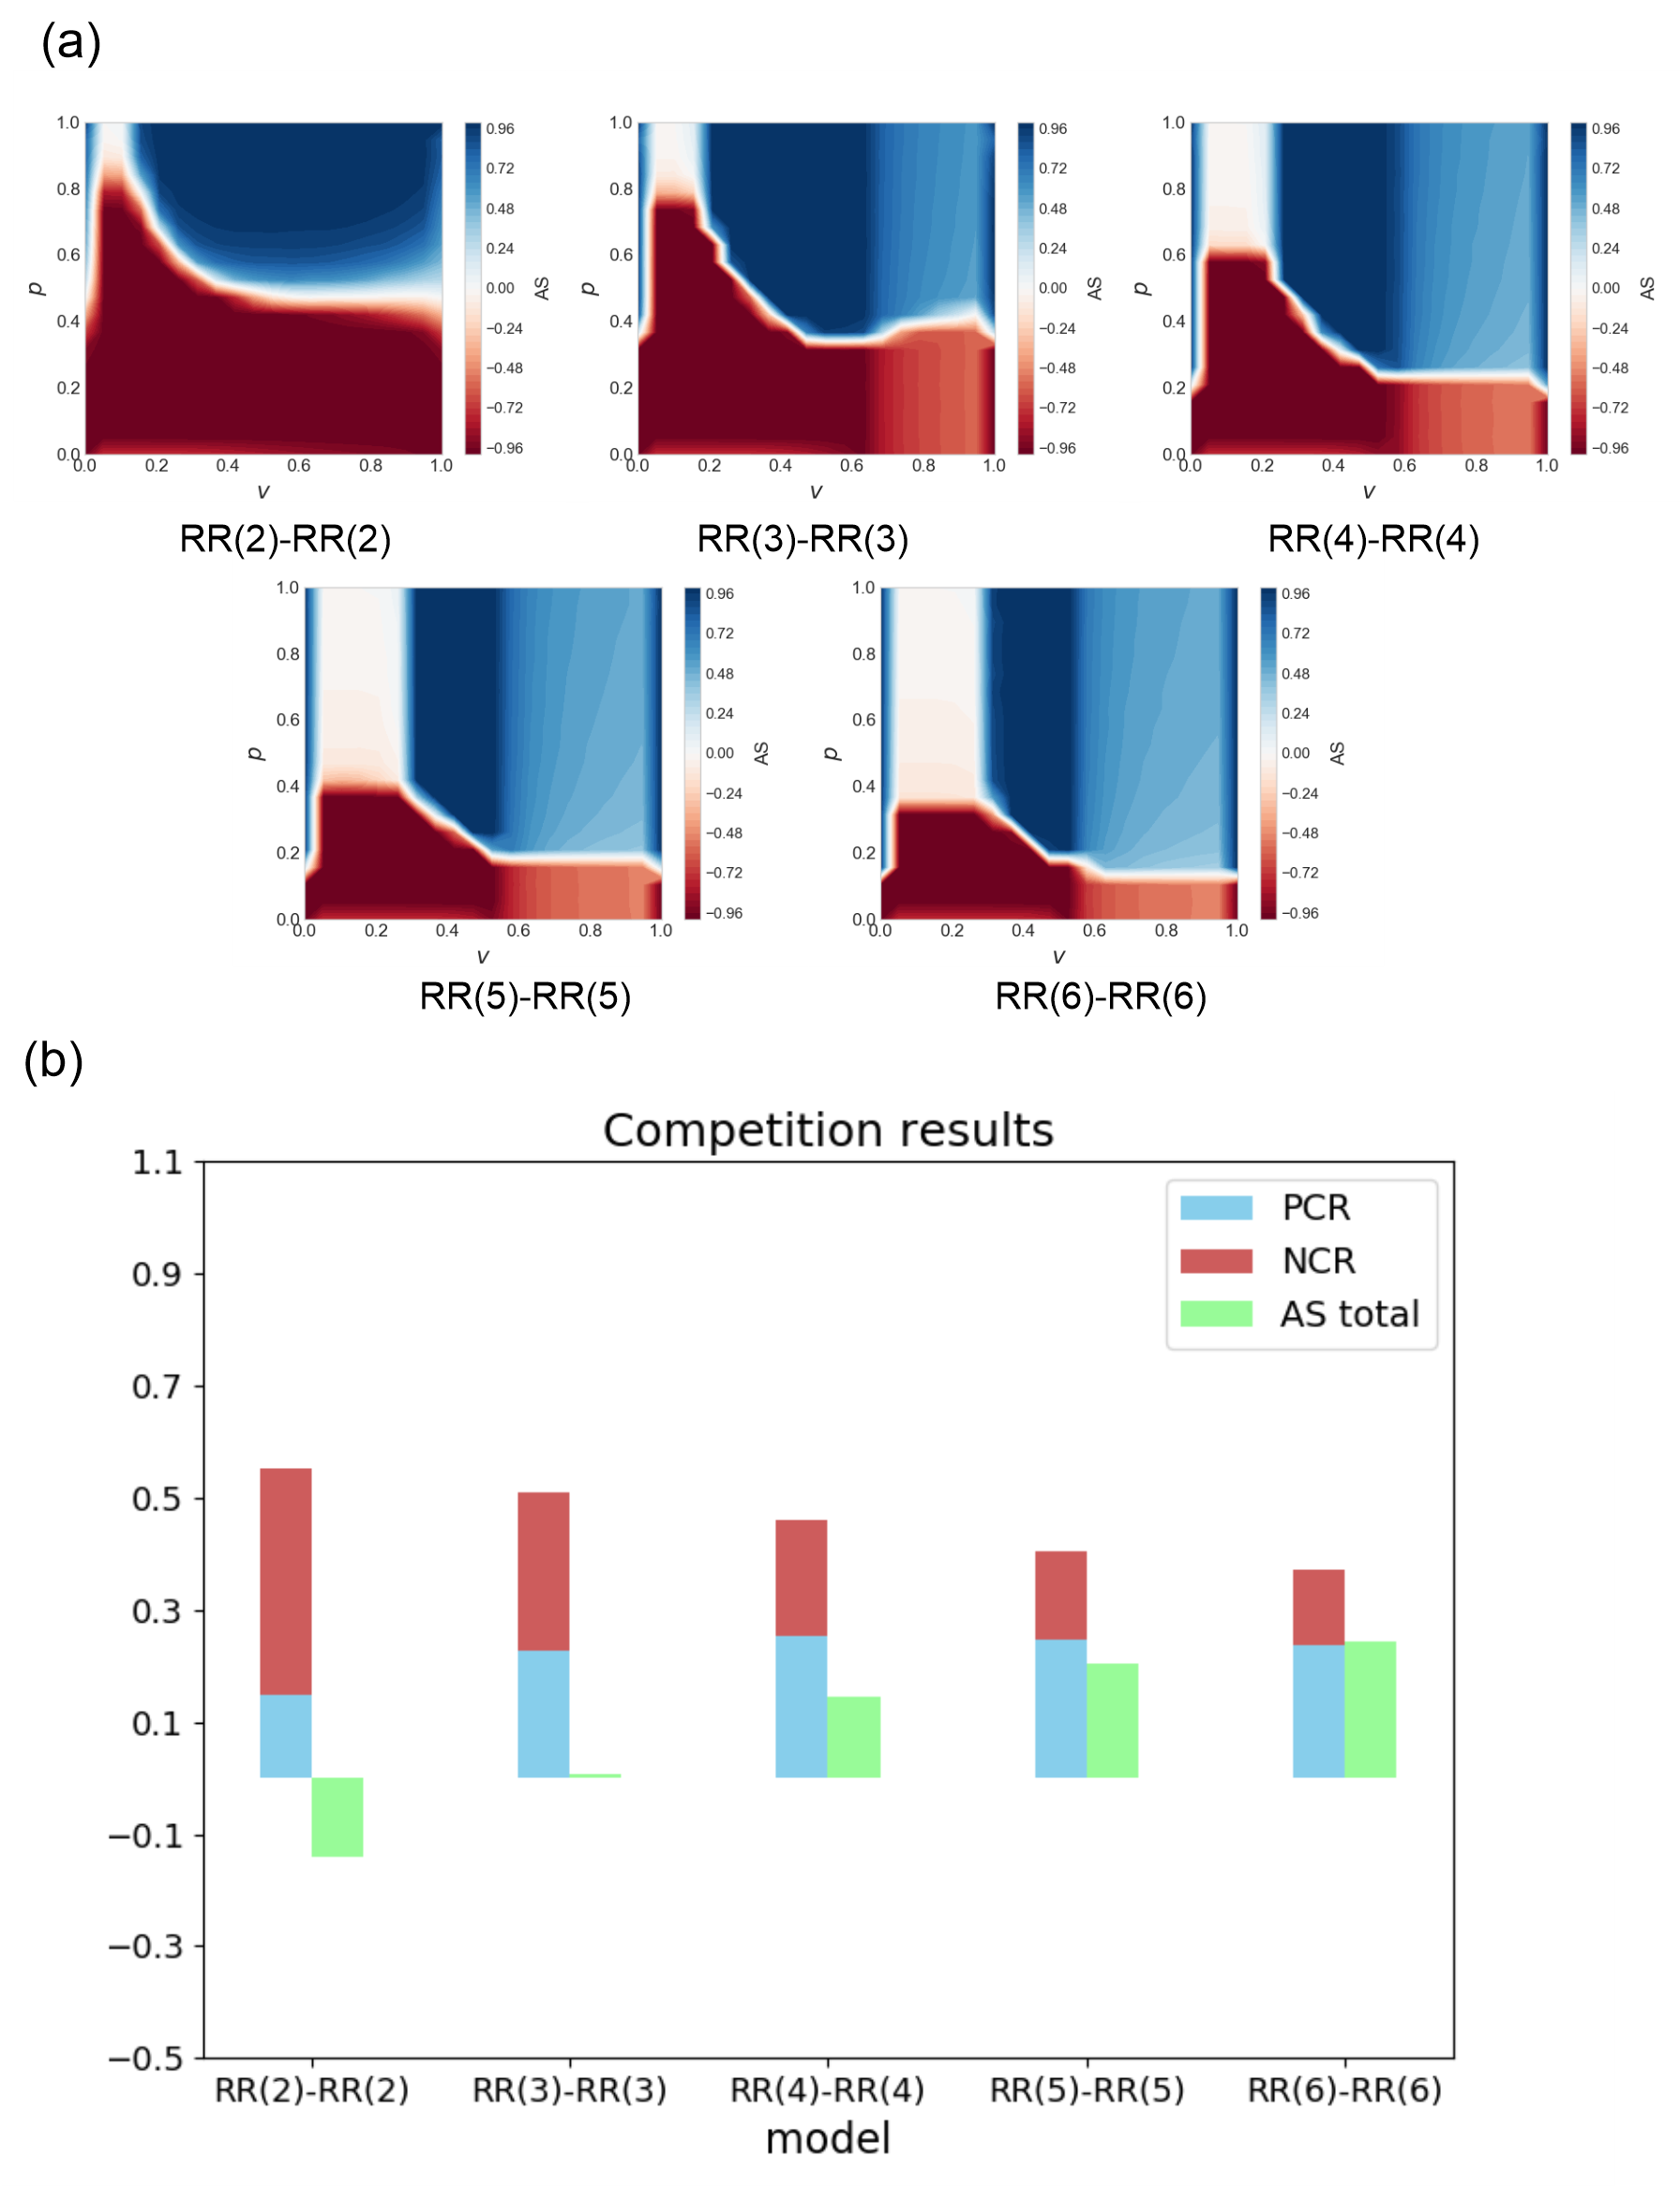
\includegraphics[width=\hsize]{chap3_internal_edge_two_total.png}
	\caption{Simulation results with changing internal degrees on both layers}
	\label{chap3_internal_edge_two_total}
\end{figure}
Next, it is simulated that internal degrees are changed on both layer A and layer B, such as \textit{RR(2)-RR(2), RR(3)-RR(3), RR(4)-RR(4), RR(5)-RR(5)} and \textit{RR(6)-RR(6)}. Through these simulations, it would be found out that how total internal degrees on both layer A and layer B affect the interconnected network.
Fig.~\ref{chap3_internal_edge_two_total} shows the influence of internal degrees on both layers. As the total number of internal degrees is increased, \textit{CR} is inversely decreased, and the ratio of positive consensus(blue area) is increased, but the ratio of negative consensus(red area) is decreased. It can be analyzed that a decrease in \textit{CR} is caused by increase in internal degrees on layer B, and an increase in ratio of \textit{PCR} is brought out by an increase in internal degrees on layer A. But, when the total number of internal degrees is increased, \textit{PCR, NCR, CR} indexes are decreased. It can be analyzed that too many internal degrees on both layers make it hard to reach consensus. 
\begin{figure}[!htb]
	\centering
	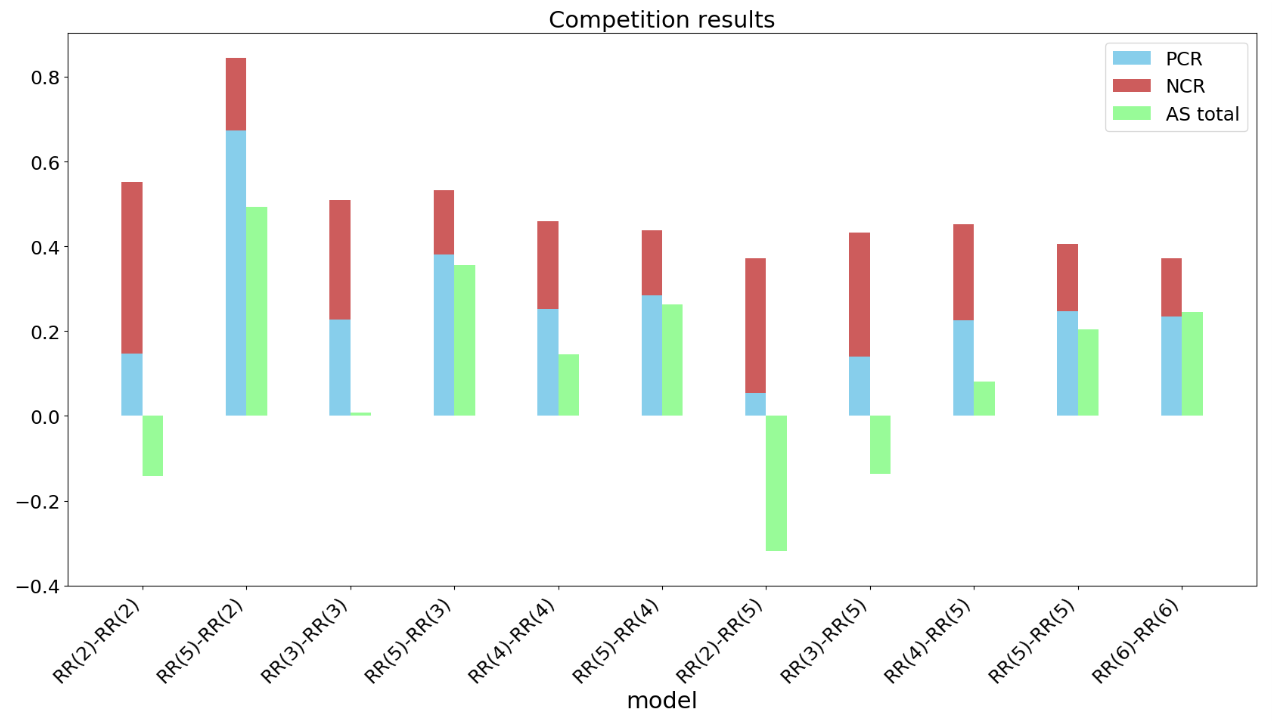
\includegraphics[width=\hsize]{chap3_internal_edge_AB_total.png}
	\caption{Total results with different internal degrees on two layers}
	\label{chap3_internal_edge_AB_total}
\end{figure}
In summary, 3 main simulations are implemented to find out the influence of internal degrees on interconnected network. First, the number of internal degrees on layer A are changed, and it is found out that the number of internal degrees on layer A has the tendency to keep positive state and to change negative state into positive state. Second, the number of internal degrees on layer B are switched, and it is found out that the number of internal degrees on layer B has the tendency to hinder positive consensus state and has the inverse relation with \textit{CR}. Third, the number of internal degrees on both layers are changed, and it is found out that too many internal degrees make it hard to reach consensus. Fig.~\ref{chap3_internal_edge_AB_total} shows the result for all simulations. 
\begin{figure}[!htb]
	\centering
	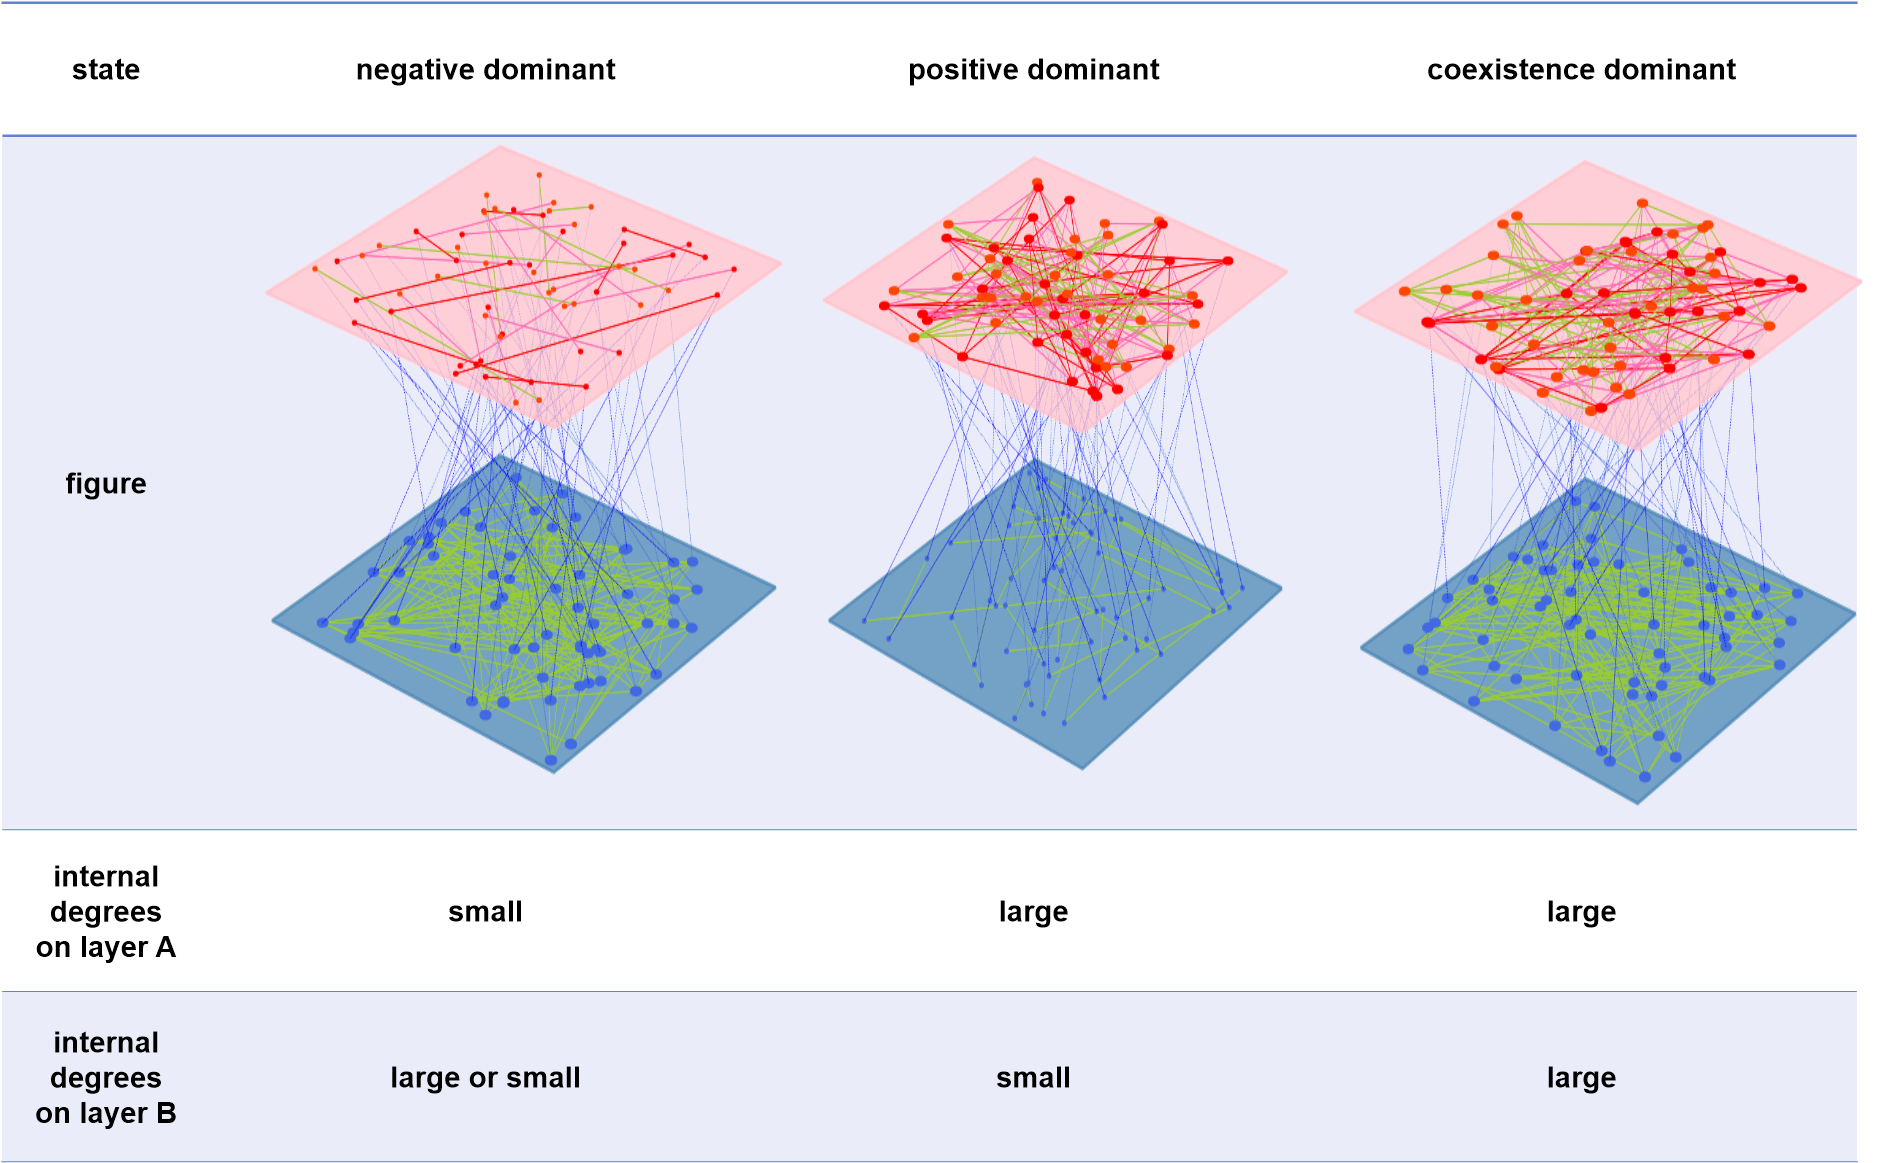
\includegraphics[width=\hsize]{chap3_internal_edge_summary.png}
	\caption{Categorizing network state according to internal degrees on two layers}
	\label{chap3_internal_edge_summary}
\end{figure}
Through these simulation results, we can analyze that how network state is changed according to the number of internal degrees. So, several conclusions can be arranged as shown in Fig.~\ref{chap3_internal_edge_summary}.  First, it is easy to reach negative consensus when the internal degrees on layer A is relatively small(the internal degrees on layer B doesn't matter). Second, it is easy to make positive consensus when the internal degrees on layer A is relatively large and the internal degrees on layer B is relatively small. Third, social conflict can be caused when the internal degrees on both layers are too large.  

\section{Competition on networks with different structures}
\begin{figure}[!htb]
	\centering
	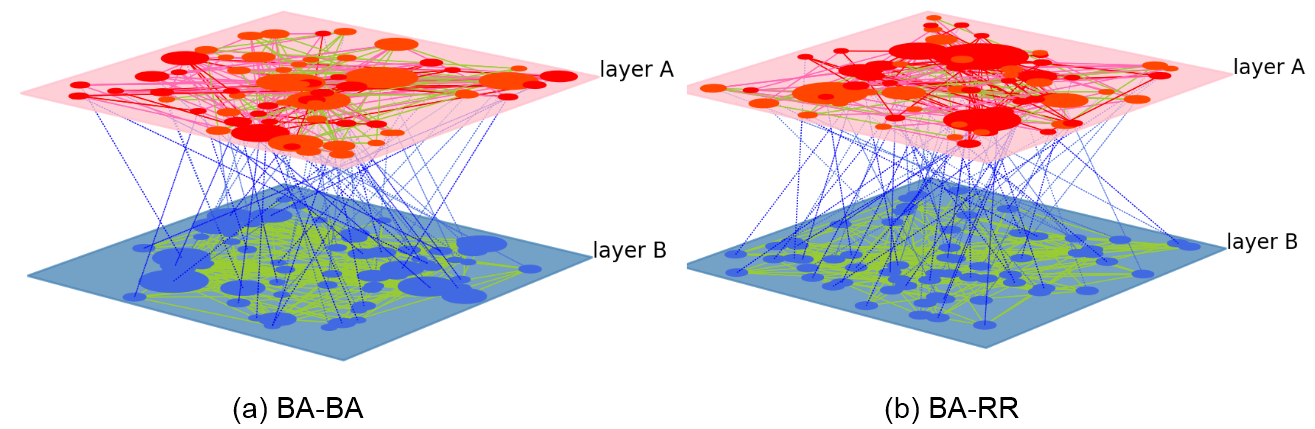
\includegraphics[width=\hsize]{chap3_changing_structure_type.png}
	\caption{Competition on interconnected networks with different structures}
	\label{chap3_changing_structure_type}
\end{figure}
So far, each layer of the interconnected network consisted of \textit{RR(random regular networks)} that has the same number of edges for each node. Now, the simulation would be implemented on different network type. Here, we use \textit{Barabasi-Albert network(BA)} structure as introduced in \parencite{barabasi1999}. \textit{Barabasi-Albert(BA)} network has $N$ nodes with attaching new nodes each with $K$ edges that are preferentially attached to existing nodes with high degrees. But, there is no change on external degree, which would be fixed to only $1$.
\begin{figure}[!htb]
	\centering
	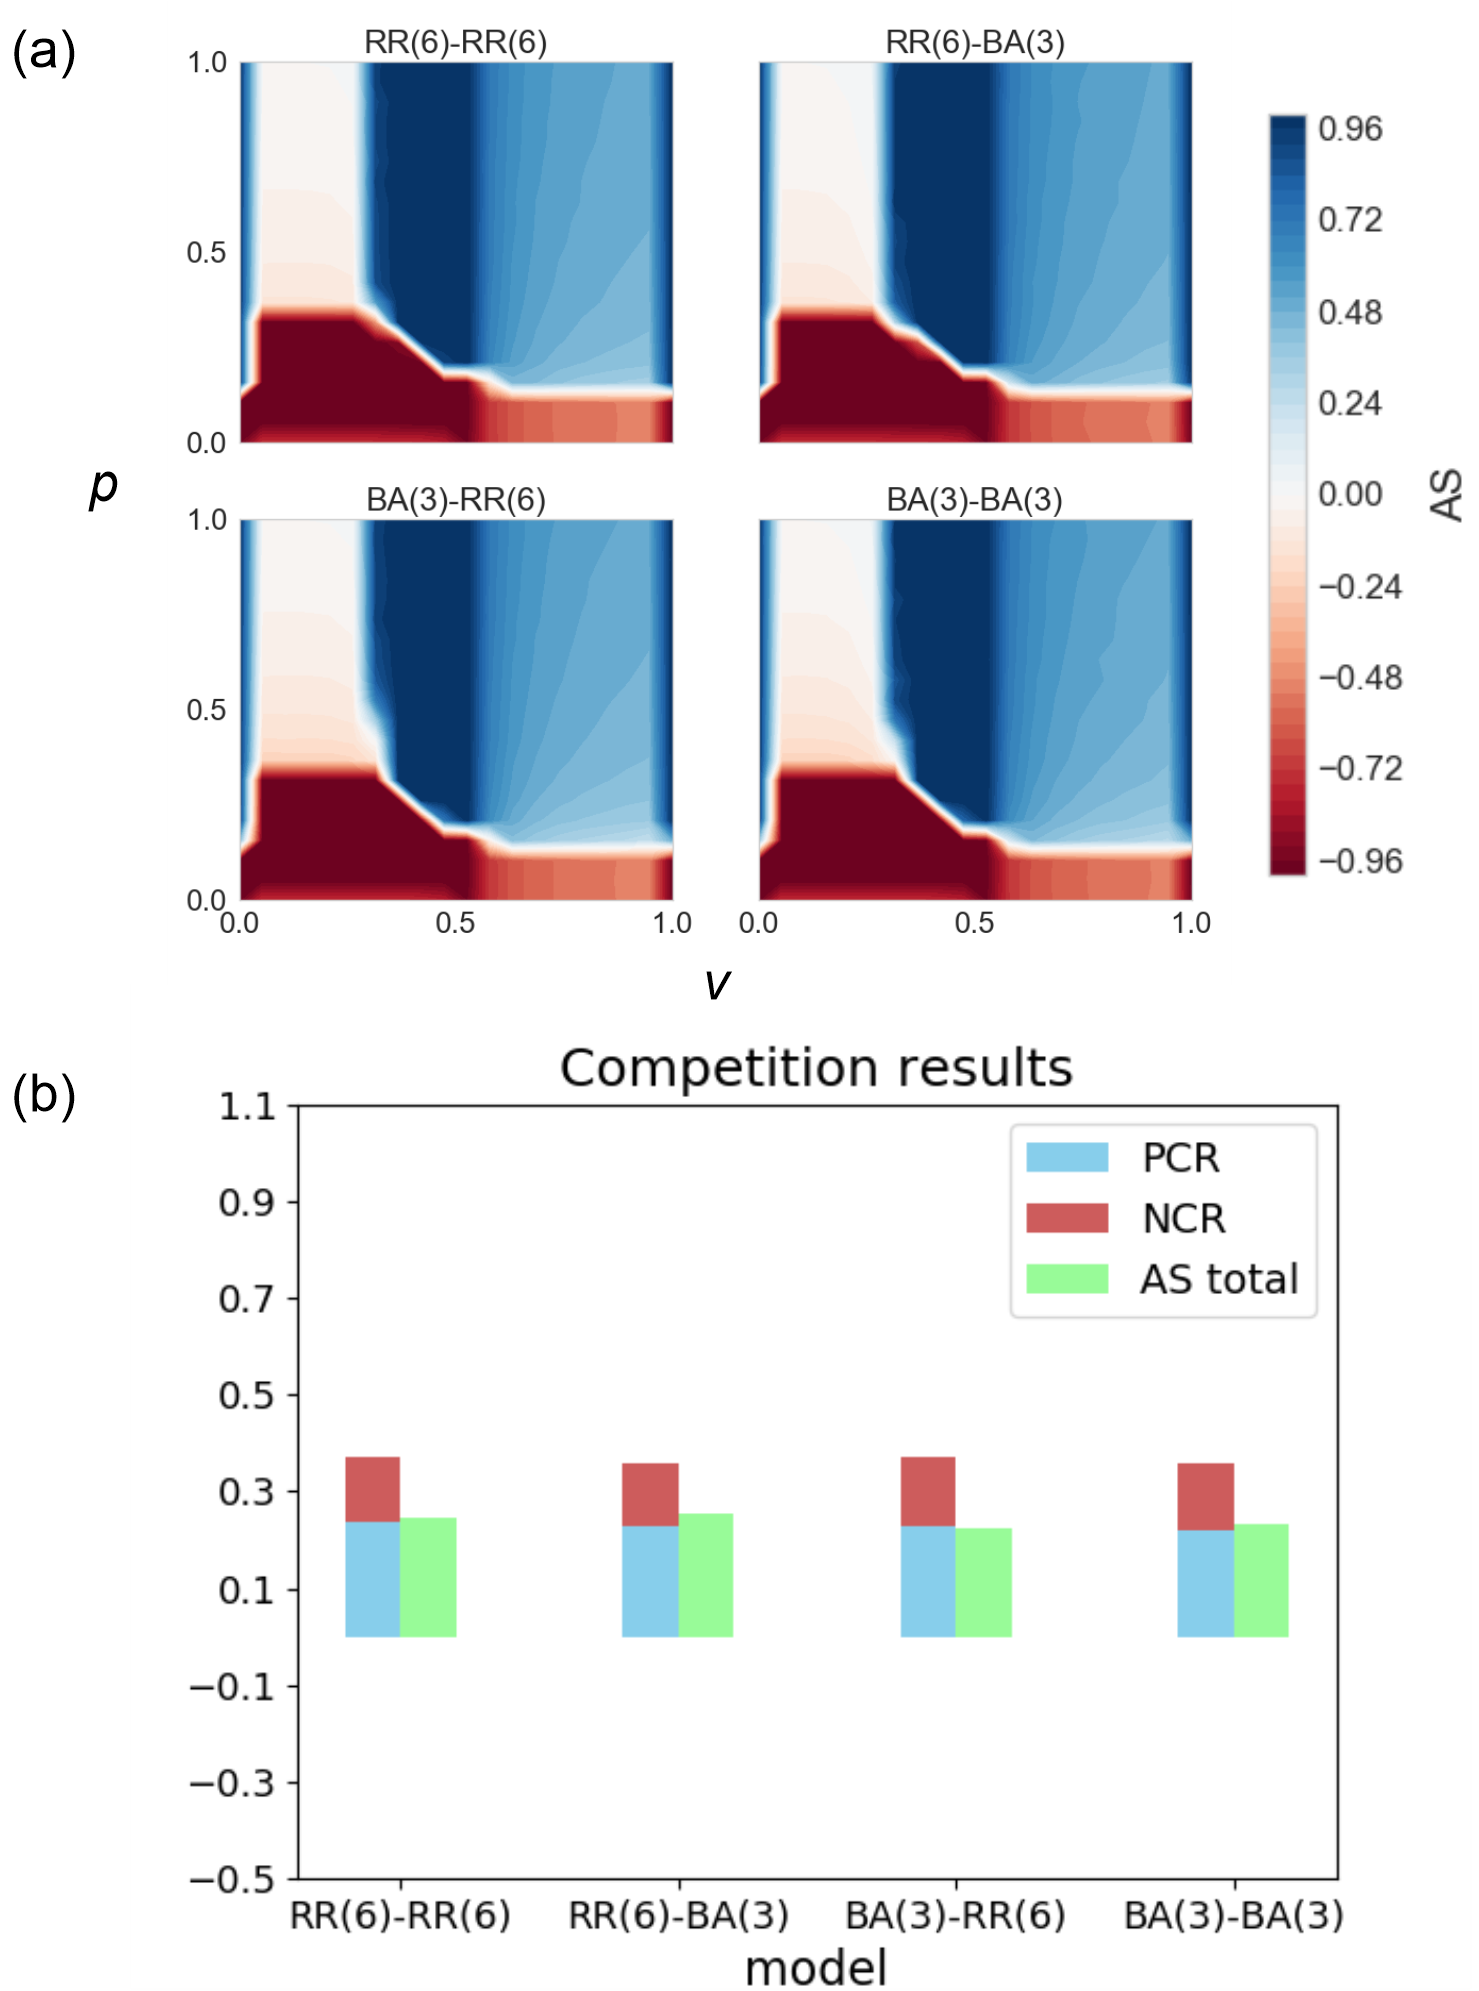
\includegraphics[width=\hsize]{chap3_changing_network_type11.png}
	\caption{Simulation results with different network types}
	\label{chap3_changing_network_type1}
\end{figure}
To evaluate the influence of network structure, 4 simulations are implemented with switching network structures. The \textit{BA} or \textit{RR} network is applied for both layers or switched on each layer. To restrain the influence of internal degree, the number of internal edges in \textit{BA} is set up to be similar with the number of internal edges in \textit{RR}. The number of internal edges in \textit{BA} is $6,135$, and the number of internal edges in \textit{RR} is $6,144$. 
\begin{figure}[!htb]
	\centering
	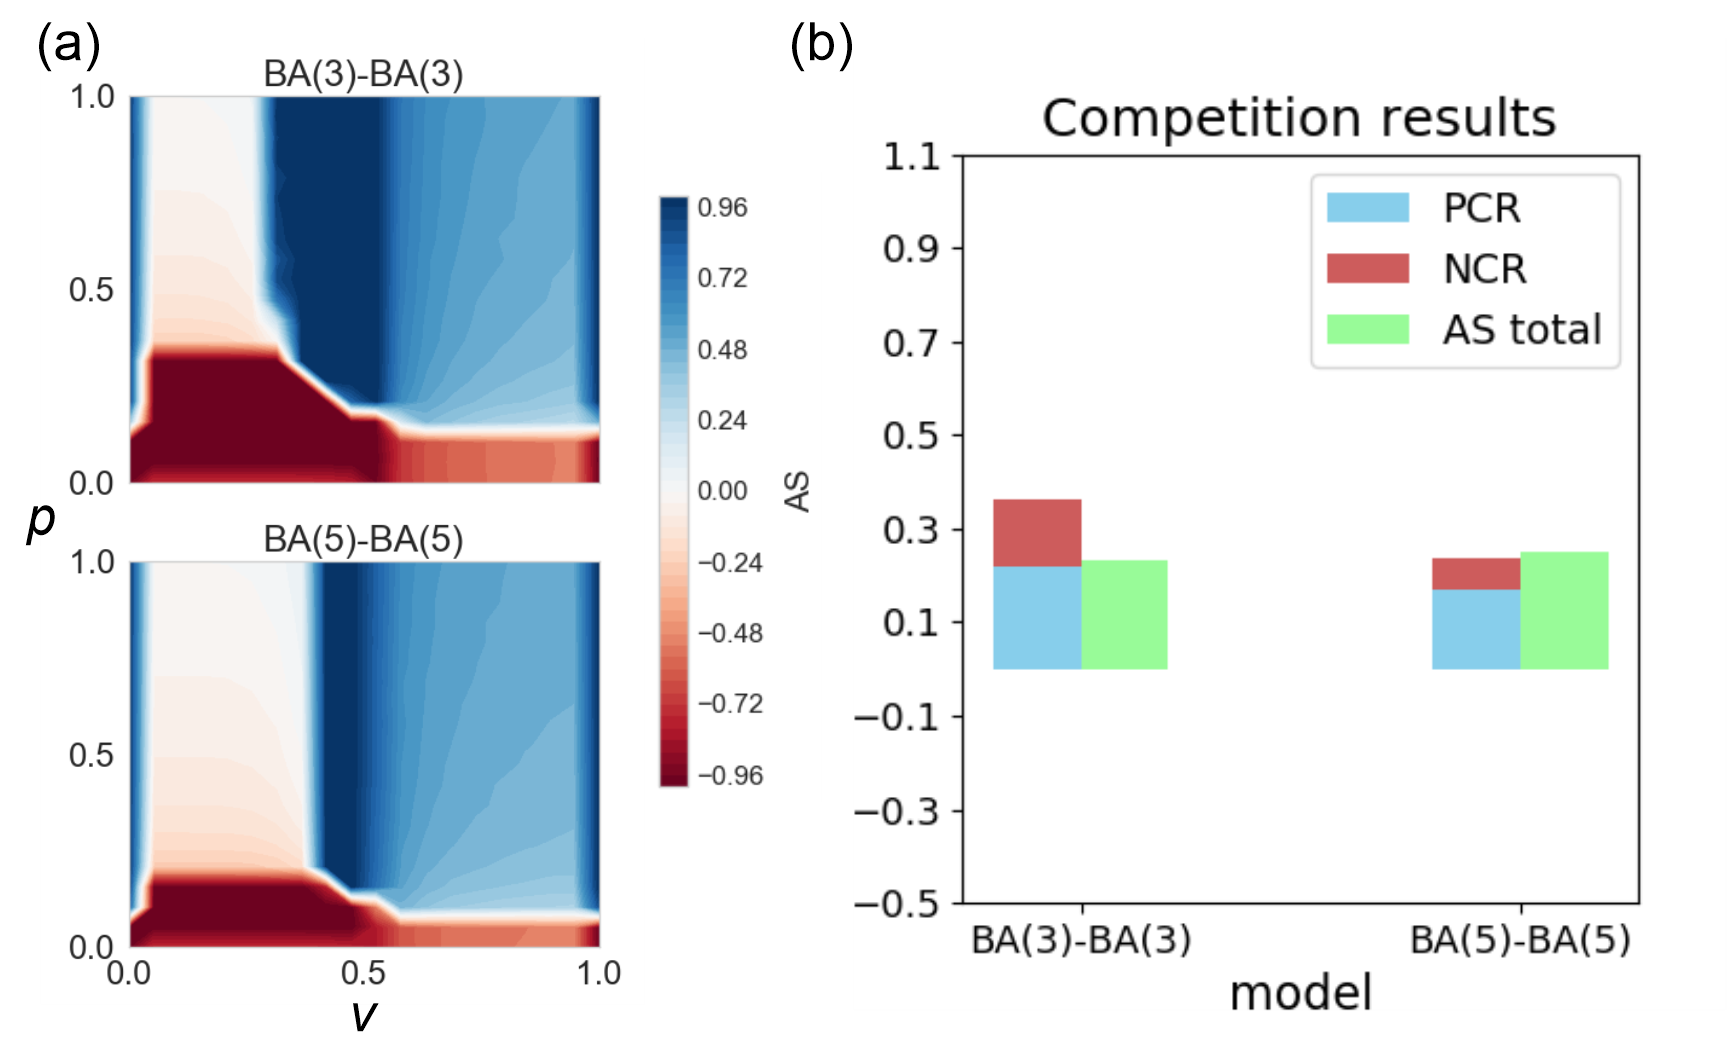
\includegraphics[width=\hsize]{chap3_changing_network_type2.png}
	\caption{BA-BA networks with changing internal degrees}
	\label{chap3_changing_network_type2}
\end{figure}
The simulation results are shown in Fig.~\ref{chap3_changing_network_type1}. The results of all simulations have almost the same features. The gap of \textit{PCR, NCR} and \textit{CR} is less than 0.02. The structure of network make no obvious difference of consensus results. Next, the number of internal edges would be increased on the network, where consists of two \textit{BA}. It would be found out that how the number of internal edges work on the network type which is different with \textit{RR}. 2 models, \textit{BA(3)-BA(3)} and \textit{BA(5)-BA(5)} would be simulated. \textit{BA(3)-BA(3)} model has $6,135$ internal edges on each layer, and \textit{BA(5)-BA(5)} model has $10,215$ internal edges on each layer. 

As shown in Fig.~\ref{chap3_changing_network_type2}, BA(5)-BA(5) has more coexistence area because of too many internal edges. The influence of internal and external degrees is more important to change network state and make consensus than the influence of network type. However, If there are stubborn nodes on networks, the simulation results would be changed because node centrality of stubborn nodes would be changed according to network type. Finding key nodes on \textit{BA} network would be simulated and analyzed in chapter.\ref{chap:finding key nodes on two layer networks}.

\section{Conclusion}
Various simulations have been simulated to find out the role of internal and external degrees and the influence of network types. All results of simulations are shown in Table.~\ref{Consensus properties of Simulation Models}. 
\begin{table}[!htb]
	\scriptsize
	\centering
    \caption{Consensus properties of Simulation Models}
	\label{Consensus properties of Simulation Models}
	\begin{center}
		\begin{tabular}{c|c|c|c|c|c|c|c|c} \hline\hline
			Div                    & A nodes& B nodes & A edges & B edges & AS total  & PCR    & NCR    & CR       \\ \hline \hline
			RR(2)-RR(5)            & 2,048  & 2,048   & 2,048   & 5,120   & -0.3186   & 0.0550 & 0.3175 & 0.3725   \\ \hline
			RR(3)-RR(5)            & 2,048  & 2,048   & 3,072   & 5,120   & -0.1368   & 0.1400 & 0.2925 & 0.4325   \\ \hline
			RR(4)-RR(5)            & 2,048  & 2,048   & 4,096   & 5,120   &  0.0804   & 0.2250 & 0.2275 & 0.4525   \\ \hline
			RR(5)-RR(2)            & 2,048 	& 2,048   & 5,120   & 2,048   &  0.4927   & 0.6725 & 0.1725 & 0.8450   \\ \hline	
			RR(5)-RR(3)            & 2,048 	& 2,048   & 5,120   & 3,072   &  0.3555   & 0.3800 & 0.1525 & 0.5325   \\ \hline
			RR(5)-RR(4)            & 2,048  & 2,048   & 5,120   & 4,096   &  0.2633   & 0.2850 & 0.1525 & 0.4375   \\ \hline
			RR(2)-RR(2)            & 2,048  & 2,048   & 2,048   & 2,048   & -0.1412   & 0.1475 & 0.4050 & 0.5525   \\ \hline
			RR(3)-RR(3)            & 2,048  & 2,048   & 3,072   & 3,072   &  0.0084   & 0.2275 & 0.2825 & 0.5100   \\ \hline
			RR(4)-RR(4)            & 2,048  & 2,048   & 4,096   & 4,096   &  0.1448   & 0.2525 & 0.2075 & 0.4600   \\ \hline
			RR(5)-RR(5)            & 2,048  & 2,048   & 5,120   & 5,120   &  0.2034   & 0.2475 & 0.1575 & 0.4050   \\ \hline
			RR(6)-RR(6)            & 2,048  & 2,048   & 6,144   & 6,144   &  0.2444   & 0.2350 & 0.1375 & 0.3725   \\ \hline
			RR(6)-BA(3)            & 2,048 	& 2,048   & 6,144   & 6,135   &  0.2541   & 0.2275 & 0.1300 & 0.3575   \\ \hline 
			BA(3)-RR(6)            & 2,048 	& 2,048   & 6,135   & 6,144   &  0.2242   & 0.2300 & 0.1425 & 0.3725   \\ \hline
			BA(3)-BA(3)            & 2,048 	& 2,048   & 6,135   & 6,135   &  0.2329   & 0.2200 & 0.1400 & 0.3600   \\ \hline
			BA(5)-BA(5)            & 2,048 	& 2,048   & 10,215  & 10,215  &  0.2496   & 0.1675 & 0.0675 & 0.2350   \\ \hline
			HM(2)  				   & 2,048 	& 1,024   & 5,120   & 2,560   &  0.3073   & 0.3275 & 0.1425 & 0.4700   \\ \hline    
			HM(4) 				   & 2,048 	&  512    & 5,120   & 1,280   &  0.4128   & 0.4125 & 0.1275 & 0.5400   \\ \hline
			HM(8)  				   & 2,048 	&  256    & 5,120   & 640     &  0.4846   & 0.4925 & 0.1150 & 0.6075   \\ \hline
			HM(16)				   & 2,048 	&  128    & 5,120   & 320     &  0.5610   & 0.5800 & 0.1100 & 0.6900   \\ \hline
			HM(32) 				   & 2,048 	&   64    & 5,120   & 160     &  0.5959   & 0.6275 & 0.1025 & 0.7300   \\ \hline
			HM(64) 				   & 2,048 	&   32    & 5,120   & 80      &  0.6185   & 0.6775 & 0.1025 & 0.7800   \\ \hline 
			HM(128) 			   & 2,048 	&   16    & 5,120   & 40      &  0.6379   & 0.7350 & 0.0900 & 0.8250   \\ \hline 
			HM(256) 			   & 2,048 	&    8    & 5,120   & 20      &  0.6454   & 0.7675 & 0.0900 & 0.8575   \\ \hline 
			 \hline
		\end{tabular}
	\end{center}
\end{table} 
Through the simulation results, several facts would be arranged like the followings. If there are no stubborn nodes, network types do not make different result for network state and consensus. But, we can provide three conclusions about the roles of internal and external degrees. First, hierarchical models show that it is easy to make consensus on both layers when the number of external edges in decision making layer is more than opinion layer. Second, the number of internal edges on layer A has the tendency to keep positive state and to change negative state into positive state. Third, the number of internal edges on layer B has the tendency to hinder positive consensus state. Fourth, too many internal edges on each layer can cause inner conflict, and that makes it hard to have consensus state. We could apply these facts to make network structures or organization in real world. 
%# -*- coding: utf-8-unix -*-
% !TEX program = xelatex
% !TEX root = ../thesis.tex
% !TEX encoding = UTF-8 Unicode
%%==================================================
%% chapter02.tex for SJTU Master Thesis
%% based on CASthesis
%% modified by wei.jianwen@gmail.com
%% Encoding: UTF-8
%%==================================================

\chapter{Competition on two layer with time-related updating rules}
\label{chap:competition on two layer with time-related updating rules}
In this chapter, we would control dynamics orders between layers and time-related updating rules of nodes states. With changing dynamics orders and time-related updating rules, it would be investigated how the states of network are changed.
Here, each layer consists of \textit{Barabasi-Albert(BA)} network that has $N$ nodes with attaching new nodes each with $K$ edges that are preferentially attached to existing nodes with high degree as introduced in \parencite{barabasi1999}. Each node of one layer is connected with a random node on the other layer. This means each node has only $1$ external un-directed edge. Simulations are performed on network with $N=2048$, and $K=3$.

When considering dynamics orders and time-related updating rules on two-layer networks, there are many ways to update the state of nodes. Dynamics orders of two layer can be considered whether layer A works first or layer B works first or both layers work together. And, orders of nodes can be thought about whether the states of nodes are changed simultaneously or sequentially or randomly. Orders of edges connected with a node also can be deliberated whether edges are activated on a node sequentially or simultaneously or randomly. But, in layer B dynamics, order of edges in one node always follows simultaneous updating rule, because dynamics formula already considers states of all connected neighbor nodes simultaneously. To sum up, as shown in Table.\ref{25updating_rules}, 25 time-related updating rules would be considered according to layers, nodes and edges. 
\begin{table}[htp]
	\scriptsize
	\begin{center}
		\begin{tabular}{c|c|c|c|c}
			Order of layers                                  & \multicolumn{2}{|c|}{Layer A}                                      & Layer B                & remarks   \\ \cline{2-4}
			& Order of nodes                 & Order of edges                     & Order of nodes         &  \\ \hline
			\multirow{10}{*}{Layer A $\rightarrow$ Layer B} & \multirow{4}{*}{Sequential}    & \multirow{2}{*}{Sequential}        & Sequential             & O(o, o) $\to$ D(o) \\  \cline{4-5}  
			&                                &                                    & Simultaneous           & O(o, o) $\to$ D(s) \\  \cline{3-5}     
			&                                & \multirow{2}{*}{Simultaneous}      & Sequential             & O(o, s) $\to$ D(o) \\  \cline{4-5} 
			&                                &                                    & Simultaneous           & O(o, s) $\to$ D(s) \\  \cline{2-5} 
			& \multirow{4}{*}{Simultaneous}  & \multirow{2}{*}{Sequential}        & Sequential             & O(s, o) $\to$ D(o) \\  \cline{4-5}
			&                                &                                    & Simultaneous           & O(s, o) $\to$ D(s) \\  \cline{3-5}
			&                                & \multirow{2}{*}{Simultaneous}      & Sequential             & O(s, s) $\to$ D(o) \\  \cline{4-5}
			&                                &                                    & Simultaneous           & O(s, s) $\to$ D(s) \\  \cline{2-5}
			& \multirow{2}{*}{Random}        & \multirow{2}{*}{Random}            & Sequential             & O(r, r) $\to$ D(o) \\  \cline{4-5}
			&                                &                                    & Simultaneous           & O(r, r) $\to$ D(s) \\   \hline
			\multirow{10}{*}{Layer A $\leftarrow$ Layer B}  & \multirow{4}{*}{Sequential}    & \multirow{2}{*}{Sequential}        & Sequential             & O(o, o) $\leftarrow$ D(o) \\  \cline{4-5}  
			&                                &                                    & Simultaneous           & O(o, o) $\leftarrow$ D(s) \\  \cline{3-5}     
			&                                & \multirow{2}{*}{Simultaneous}      & Sequential             & O(o, s) $\leftarrow$ D(o) \\  \cline{4-5} 
			&                                &                                    & Simultaneous           & O(o, s) $\leftarrow$ D(s) \\  \cline{2-5} 
			& \multirow{4}{*}{Simultaneous}  & \multirow{2}{*}{Sequential}        & Sequential             & O(s, o) $\leftarrow$ D(o) \\  \cline{4-5}
			&                                &                                    & Simultaneous           & O(s, o) $\leftarrow$ D(s) \\  \cline{3-5}
			&                                & \multirow{2}{*}{Simultaneous}      & Sequential             & O(s, s) $\leftarrow$ D(o) \\  \cline{4-5}
			&                                &                                    & Simultaneous           & O(s, s) $\leftarrow$ D(s) \\  \cline{2-5}
			& \multirow{2}{*}{Random}        & \multirow{2}{*}{Random}            & Sequential             & O(r, r) $\leftarrow$ D(o) \\  \cline{4-5}
			&                                &                                    & Simultaneous           & O(r, r) $\leftarrow$ D(s) \\   \hline
			\multirow{2}{*}{Layer A $\leftrightarrow$ Layer B}& \multirow{2}{*}{Simultaneous}& Sequential                         & Simultaneous           & O(s, o) $\leftrightarrow$ D(s) \\ \cline{3-5}
			&                                & Simultaneous                       & Simultaneous           & O(s, s) $\leftrightarrow$ D(s) \\ \hline
			\multirow{3}{*}{Layer A $\Leftrightarrow$ Layer B}& \multirow{2}{*}{Sequential}  & Sequential                         & Sequential             & O(o, o) $\Leftrightarrow$ D(o) \\ \cline{3-5}
			&                                & Simultaneous                       & Sequential             & O(o, s) $\Leftrightarrow$ D(o) \\ \cline{2-5}
			& Random                         & Random                             & Random                 & O(r, r) $\Leftrightarrow$ D(r) \\ \hline
			
		\end{tabular}
	\end{center}
	\caption{25 updating rules according to order of layers, nodes, and edges}
	\label{25updating_rules}
\end{table}

In table remarks, `O(o, o) $\to$ D(s)' indicates `Opinion layer(node : sequential order updating, edges : sequential order updating) $\to$ Decision Making layer(node : simultaneous updating)', that means all nodes in Opinion layer are updated with order of nodes and edges and then all nodes in Decision Making layer are updated with order of nodes and edges according to arrow direction. `O(o, o) $\Leftrightarrow$ D(o)' means that one node in Opinion layer is updated and then one node in Decision Making layer is updated until all nodes are updated.
Dynamics with 25 updating rules are simulated with parameter $p=0.4$ and $v=0.4$. Simulation results are divided by order of layers, nodes and edges. 

\section{Order of layers}
There exist two layers on interconnected network. And each layer have its own dynamics, such as \textit{M-Model} and \textit{AS-Model}. Two dynamics can be operated simultaneously or sequentially. If they act sequentially, dynamics of layer A can act first or dynamics of layer B can work previously. Otherwise, regardless of layers order, nodes of two layers can interact mutually, i.e. one node in layer A are updated and then one node in layer B are updated until all nodes are updated.  
Considering all situations, there are 4 ways in order of two layers, \textit{Layer A $\to$ Layer B, Layer A $\leftarrow$ Layer B, Layer A $\leftrightarrow$ Layer B(simultaneous), Layer A $\Leftrightarrow$ Layer B(interaction regardless of layers' order)}. 
\begin{figure}[!htb]
	\centering
	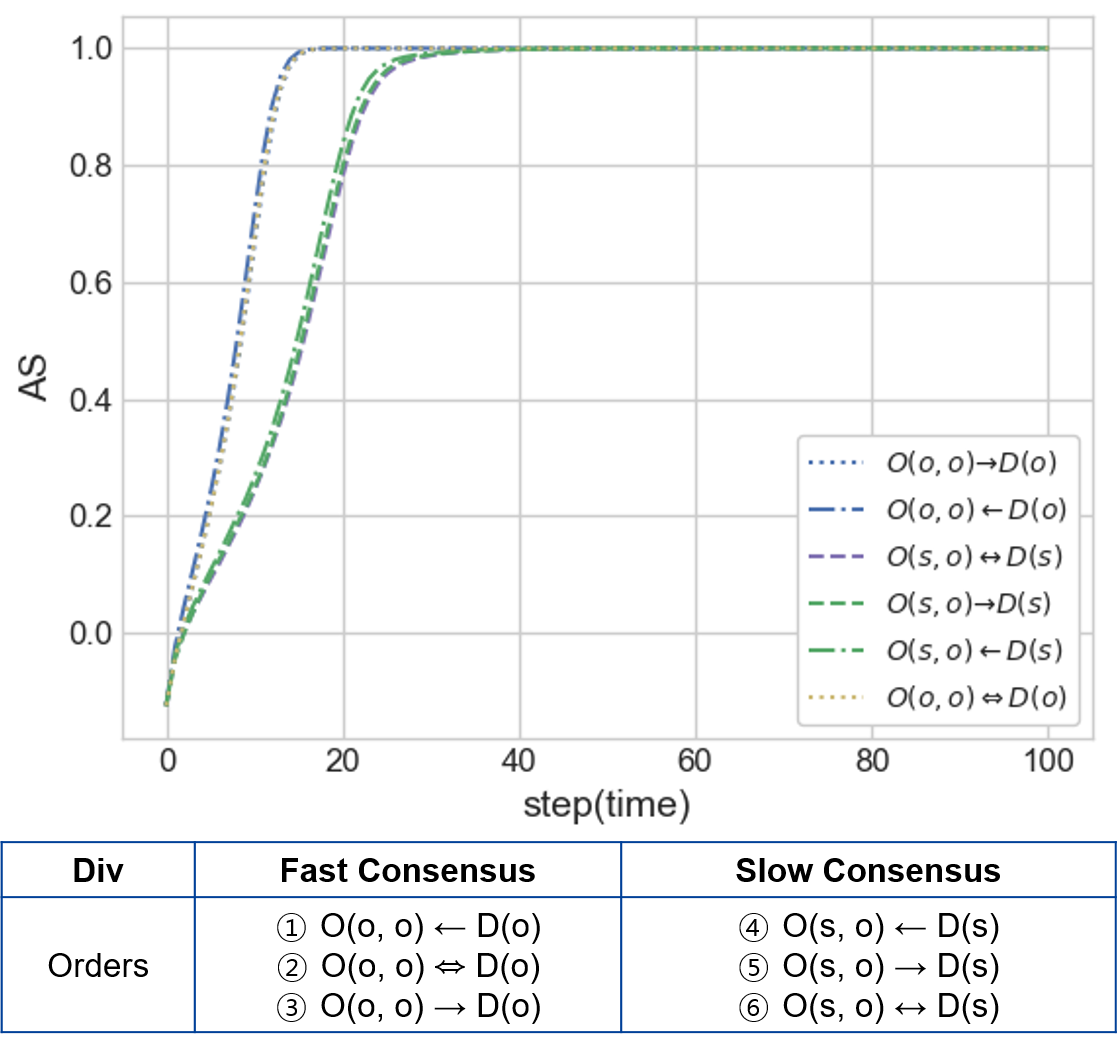
\includegraphics[width=\hsize]{chap4_layerorder.png}
	\caption{Simulation results according to orders of layers: comparison between orders of layers under same conditions such as orders of nodes and edges.}
	\label{chap4_layerorder}
\end{figure}
Fig.~\ref{chap4_layerorder} shows $4$ simulation results related to orders of layers. As seen in Fig.~\ref{layerorder}, it is shown that there is little difference according to orders of layers. Consensus time and result are almost same, though dynamics order is different. Regardless of dynamics orders, when other conditions, such as time-related updating rules of nodes and edges, are same, the dynamics results are also very similar. It could be found out that dynamics order of layers does not have an significant influence on the network state.  

\section{Order of nodes}
In the simulation model, each layer has $2048$ nodes, and each node has interactions with other nodes. Now, interaction order of nodes would be considered. One node can be updated sequentially after neighbor nodes are updated. Otherwise, every node can be updated simultaneously. And, nodes would be also updated randomly. In random order, one edge is selected randomly and updated until all edges are considered regardless of orders of nodes or edges.(For layer B, random order can not be applied because it has the formula, that is all edges of a node are considered together) So, simulations would be implemented according to $3$ orders of nodes, such as sequential order, simultaneous order and random order.  It could be thought that interaction orders of nodes are related to communication methods in real world. If networks follow sequential updating rule of nodes, communication methods of networks might be analyzed as discussion or conversation with enough time. However, if networks follow simultaneous updating rules of nodes, communication methods of networks might be analyzed as vote or election. 

\begin{figure}[!htb]
	\centering
	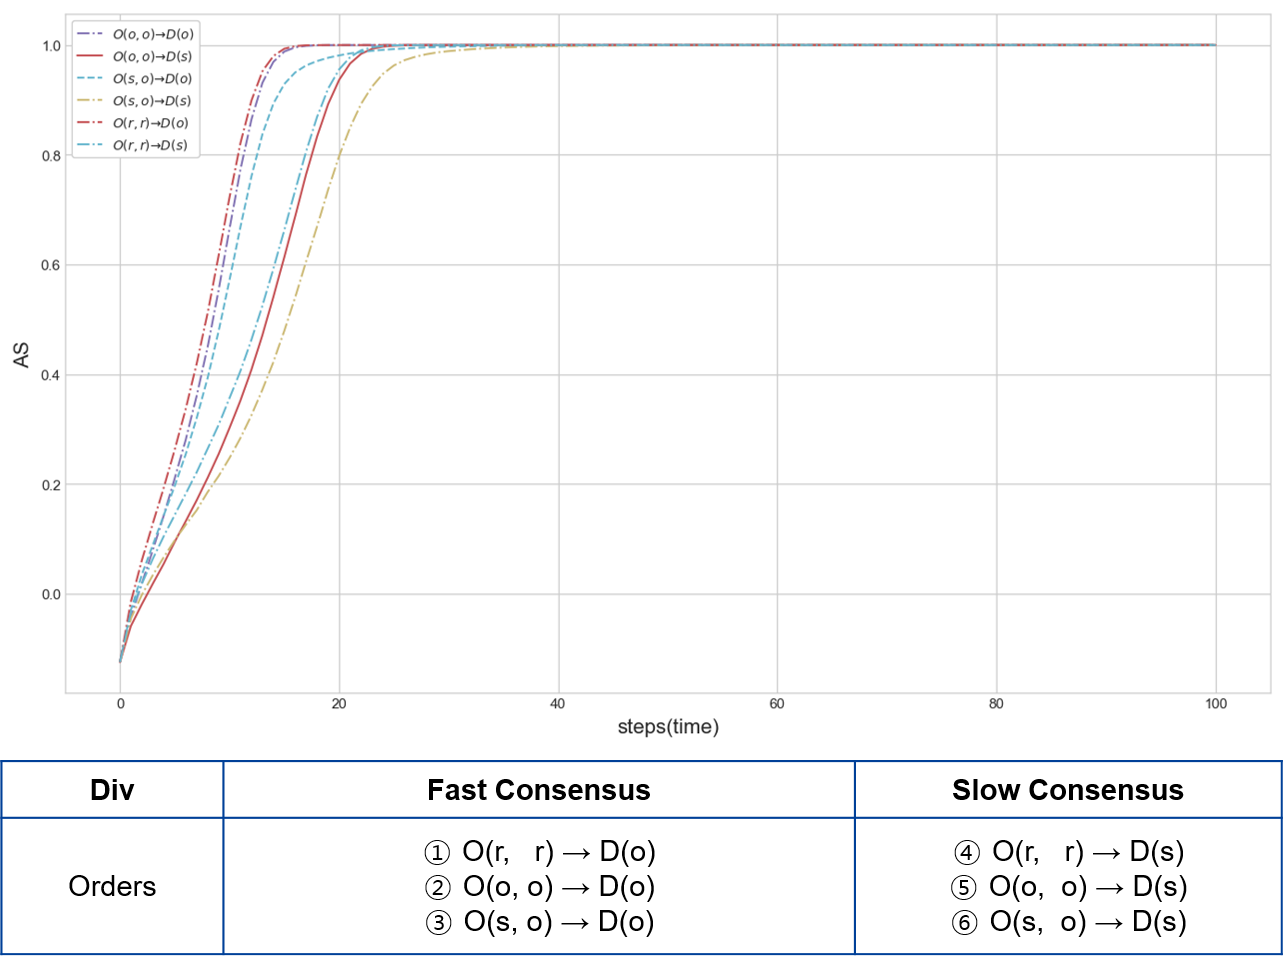
\includegraphics[width=\hsize]{figure/chap4_nodeorder.png}
	\caption{Simulation results according to orders of nodes: comparison between order of nodes under same conditions such as order of layers and edges.}
	\label{chap4_nodeorder}
\end{figure}

Fig.~\ref{chap4_nodeorder} shows simulation results according to interaction orders of nodes. The results are classified to two categories, fast consensus and slow consensus. It is shown that simultaneous interaction between nodes makes slow consensus. Simultaneous order in layer A does not make large difference with other orders in layer A, but it makes consensus slightly slow. Simultaneous interaction between nodes in layer B makes consensus slower than layer A. Random order has similar results with sequential order and does not make different states. It is found out that simultaneous order of nodes makes slow consensus and sequential order of nodes makes fast consensus. In addition, interaction order of nodes in layer B has more influence on consensus time than in layer A. To make quick social consensus, both opinion layer and decision making layer would need sequential updating rule, such as conversation and discussion.      

\section{Order of edges}
Each node has several edges connected with other nodes. Updating rules can be divided according to that edges are activated sequentially or simultaneously. If edges of each node work sequentially, a state of node is changed whenever each edge is activated. However, If edges of a node are activated simultaneously, a state of node would be changed considering all connected nodes. In real world, order of edges in one node can be analyzed as characteristics of nodes. If order of edges is sequential, the node would be analyzed as rash because the state of node is changed whenever edges are activated. If order of edges is simultaneous, the node would be analyzed as considerate because it considers all connected nodes. 

\begin{figure}[!htb]
	\centering
	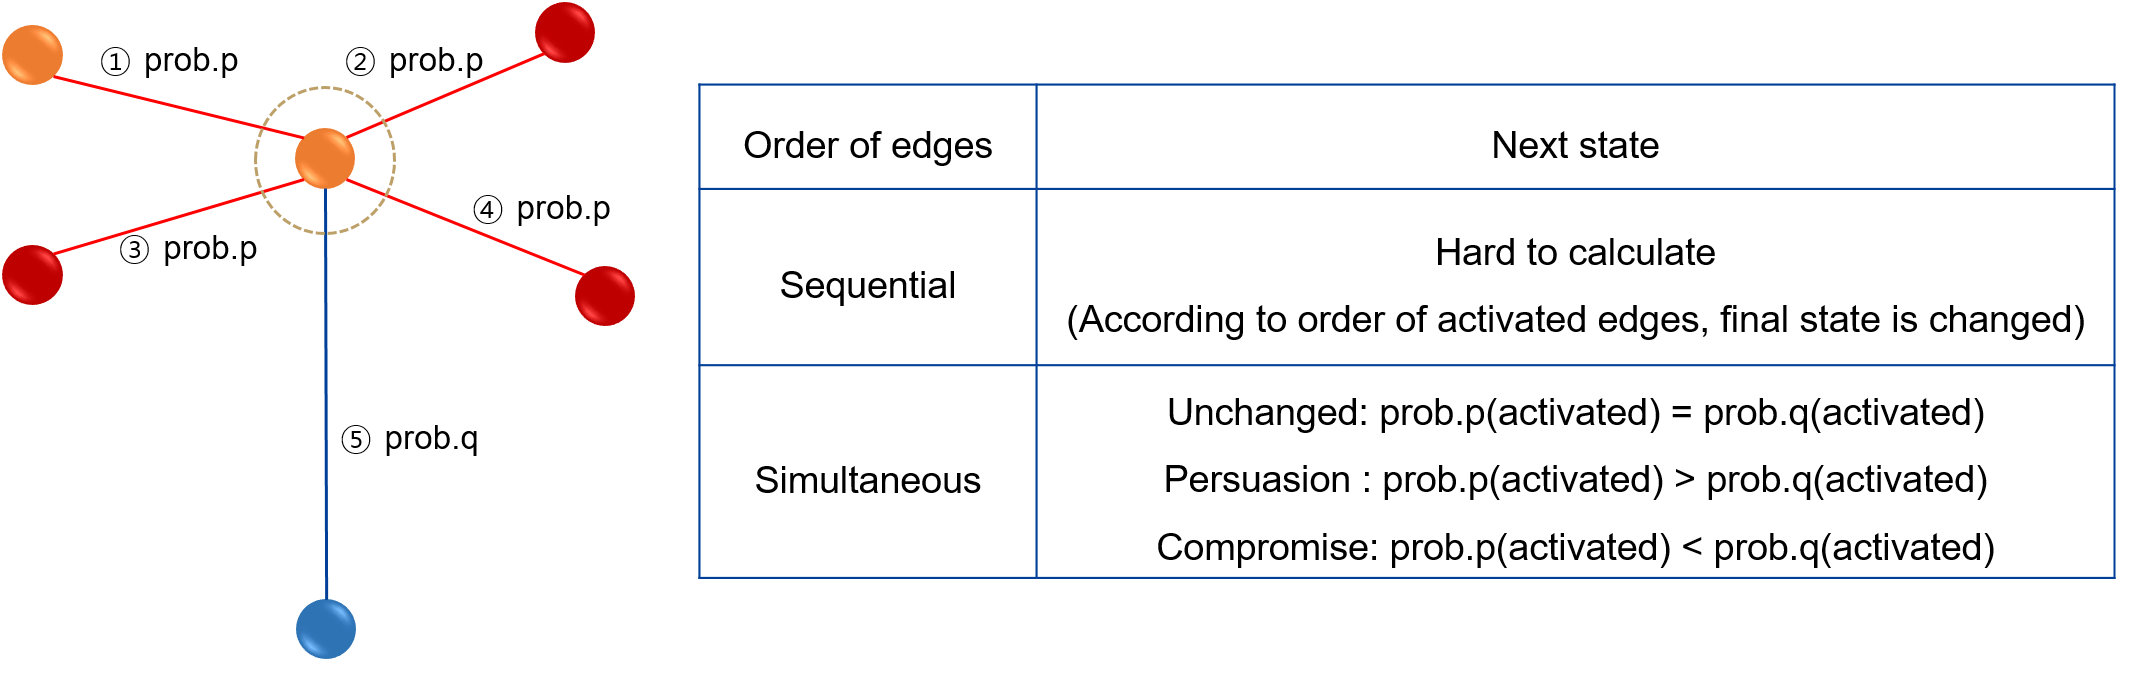
\includegraphics[width=\hsize]{figure/chap4_edgeorder_explanation.png}
	\caption{one node connected with other nodes changes its state with sequential or simultaneous order of edges}
	\label{edgeorder_explanation}
\end{figure}  
For example, considering the case that one node is connected with other nodes as shown in Fig.~\ref{edgeorder_explanation}, we can think how the state of node change. 
If the edges follow sequential updating rule, it is hard to calculate the probabilities, because the states can change according to sequential order of edges continuously. Therefore, the next states of nodes would be found by using computer simulation.
If the edges follow simultaneous updating rule, it needs some assumptions: 
\begin{enumerate}
	\item If the number of activated \textit{prob.p} is more than the number of activated \textit{prob.q}, persuasion dynamics would work. 
	\item If the number of activated \textit{prob.p} is same with the number of activated \textit{prob.q}, the state would be unchanged.
	\item If the number of activated \textit{prob.p} is less than the number of activated \textit{prob.q}, compromise dynamics would work.
\end{enumerate}

Through these assumptions, we can calculate probabilities of changing state in layer by considering all cases as these formula.  

\begin{equation}
\begin{array}{l}
K = \{ k \quad|\quad 0, \cdots ,{n^{ - {S_i}}}\}, \quad L = \{l \quad|\quad 0, \cdots ,{n^{{S_i}}}\},
\quad M = \{m \quad|\quad k-l\}, \\
{P_A}({S_i} \mapsto {{S'}_i}) = \begin{cases}
\mbox{unchanged}(k = l):\sum {{p^{{n^{ - {S_i}}}+m}} \cdot {{(1 - p)}^{{n^{{S_i}}}-m}} \cdot {}_{{n^{{S_{^i}}}}}{C_k} \cdot {}_{{n^{ - {S_{^i}}}}}{C_l}} \\
\mbox{persuasion}(k > l):\sum {{p^{{n^{ - {S_i}}}+m}} \cdot {{(1 - p)}^{{n^{{S_i}}}-m}} \cdot {}_{{n^{{S_{^i}}}}}{C_k} \cdot {}_{{n^{ - {S_{^i}}}}}{C_l}} \\
\mbox{compromise}(k < l):\sum {{p^{{n^{ - {S_i}}}+m}} \cdot {{(1 - p)}^{{n^{{S_i}}}-m}} \cdot {}_{{n^{{S_{^i}}}}}{C_k} \cdot {}_{{n^{ - {S_{^i}}}}}{C_l}} 
\end{cases}
\end{array}
\end{equation}

\begin{figure}[!htb]
	\centering
	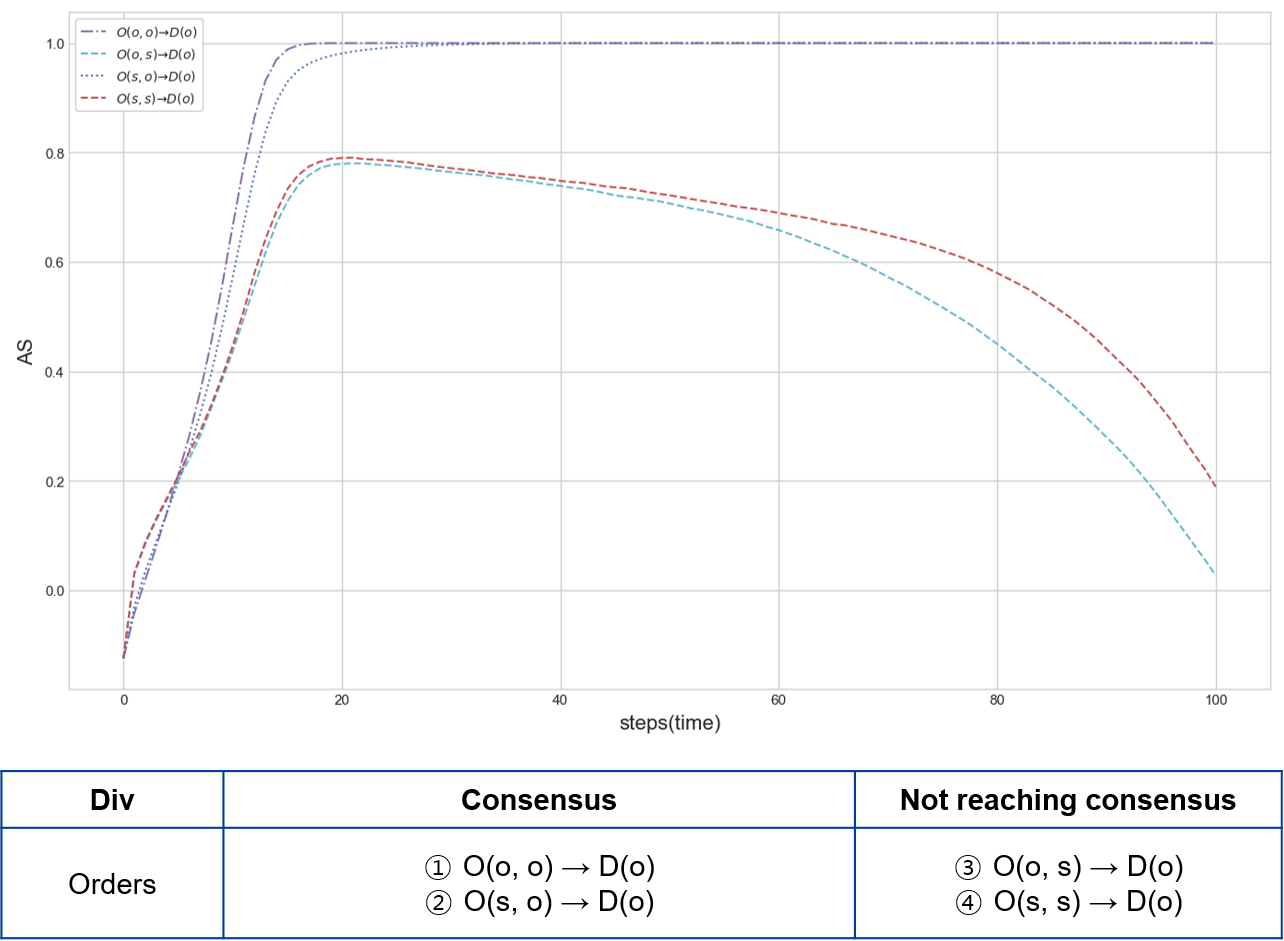
\includegraphics[width=\hsize]{figure/chap4_edgeorder.png}
	\caption{Simulation results according to orders of edges: comparison between order of edges under same conditions such as order of layers and nodes}
	\label{edgeorder}
\end{figure}

Fig.~\ref{edgeorder} shows the simulation result according to order of edges. The results could be categorized to consensus and coexistence(not reaching consensus). Sequential updating rule of edges makes consensus under the same conditions such as orders of nodes and layers, i.e. rash nodes make consensus. But simultaneous updating rule of edges makes it hard to reach consensus under the same conditions such as orders of nodes and layers, i.e. considerate nodes do not make consensus. It can be analyzed that rash node is easy to be extreme and make consensus, but considerate node is very moderate and makes it hard to reach consensus.
 
\section{Comparison and Analysis}
It is found out that there are different simulation results according to orders of layers, nodes, and edges. To sum up all time-related updating rules, they can be categorized into 3 parts, positive consensus, coexistence, and negative consensus as shown in Fig.~\ref{ordertotal}.  
\begin{figure}[!htb]
	\centering
	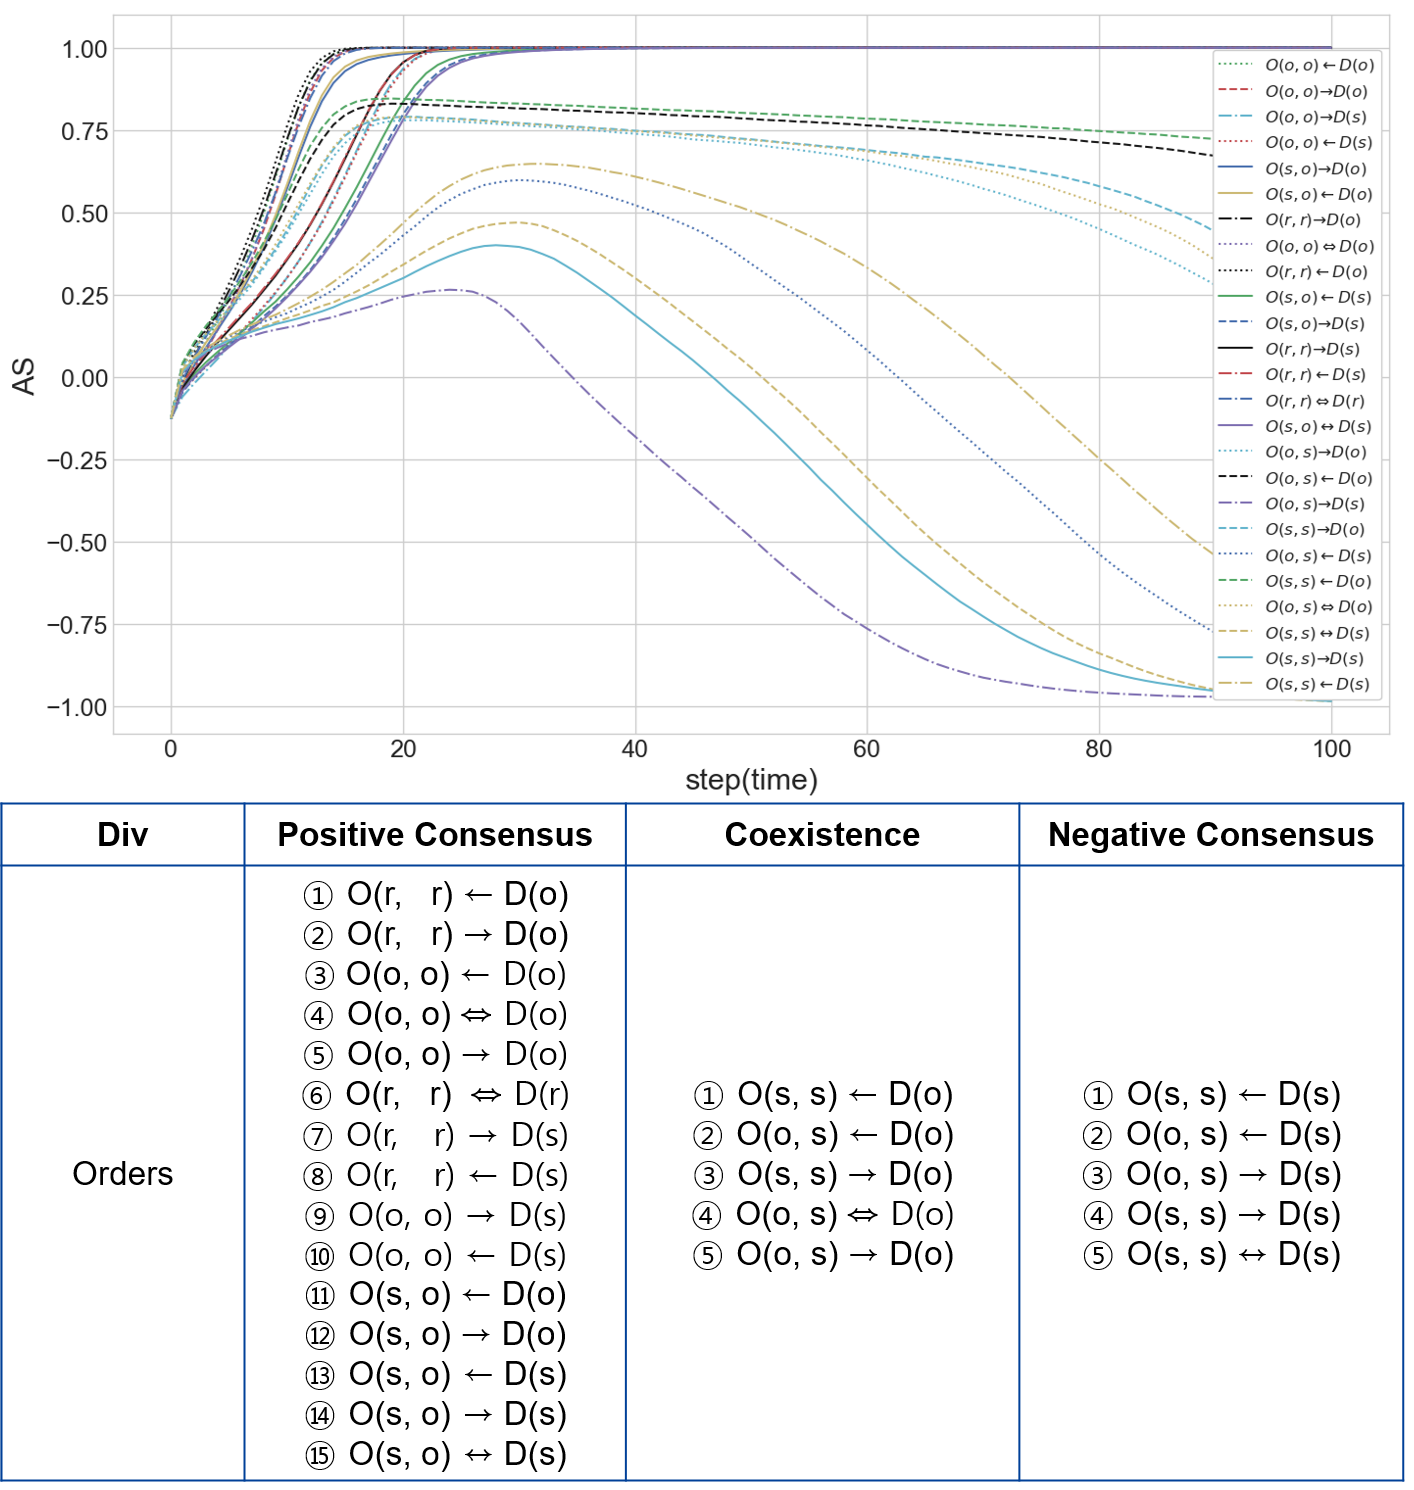
\includegraphics[width=\hsize]{figure/chap4_ordertotal.png}
	\caption{Total results of 25 updating rules with \textit{AS}}
	\label{ordertotal}
\end{figure}
To clearly classify the state of two-layers, the results can be analyzed by using \textit{CI}, that measures how close the state of network is to consensus, as shown in Fig.~\ref{ordertotal2}. There are three branch points. In the first branch point, the results are divided according to whether order of nodes in layer B is sequential or simultaneous. First branch point makes the results divided into fast convergent or slow convergent. In the second and third branch point, the results are divided according to whether order of edges in layer A is sequential or simultaneous. Second branch point makes the results divided into consensus or coexistence. Third branch point makes the results divided into positive consensus or negative consensus. To sum up, simulations results are classified into 4 categories such as fast positive consensus, slow positive consensus, coexistence and slow negative consensus. The factors that make branch points have vital influence for the state of networks. That means order of nodes(communication method) in layer B and order of edges(node characteristics) in layer A have very important role to make the state of network. It can be analyzed that communication method on decision-making layer makes fast or slow convergent for opinions and node characteristics on opinion layer makes the final state of networks such as positive consensus, negative consensus and coexistence. 

and node characteristics on opinion layer have  
\begin{figure}[!htb]
	\centering
	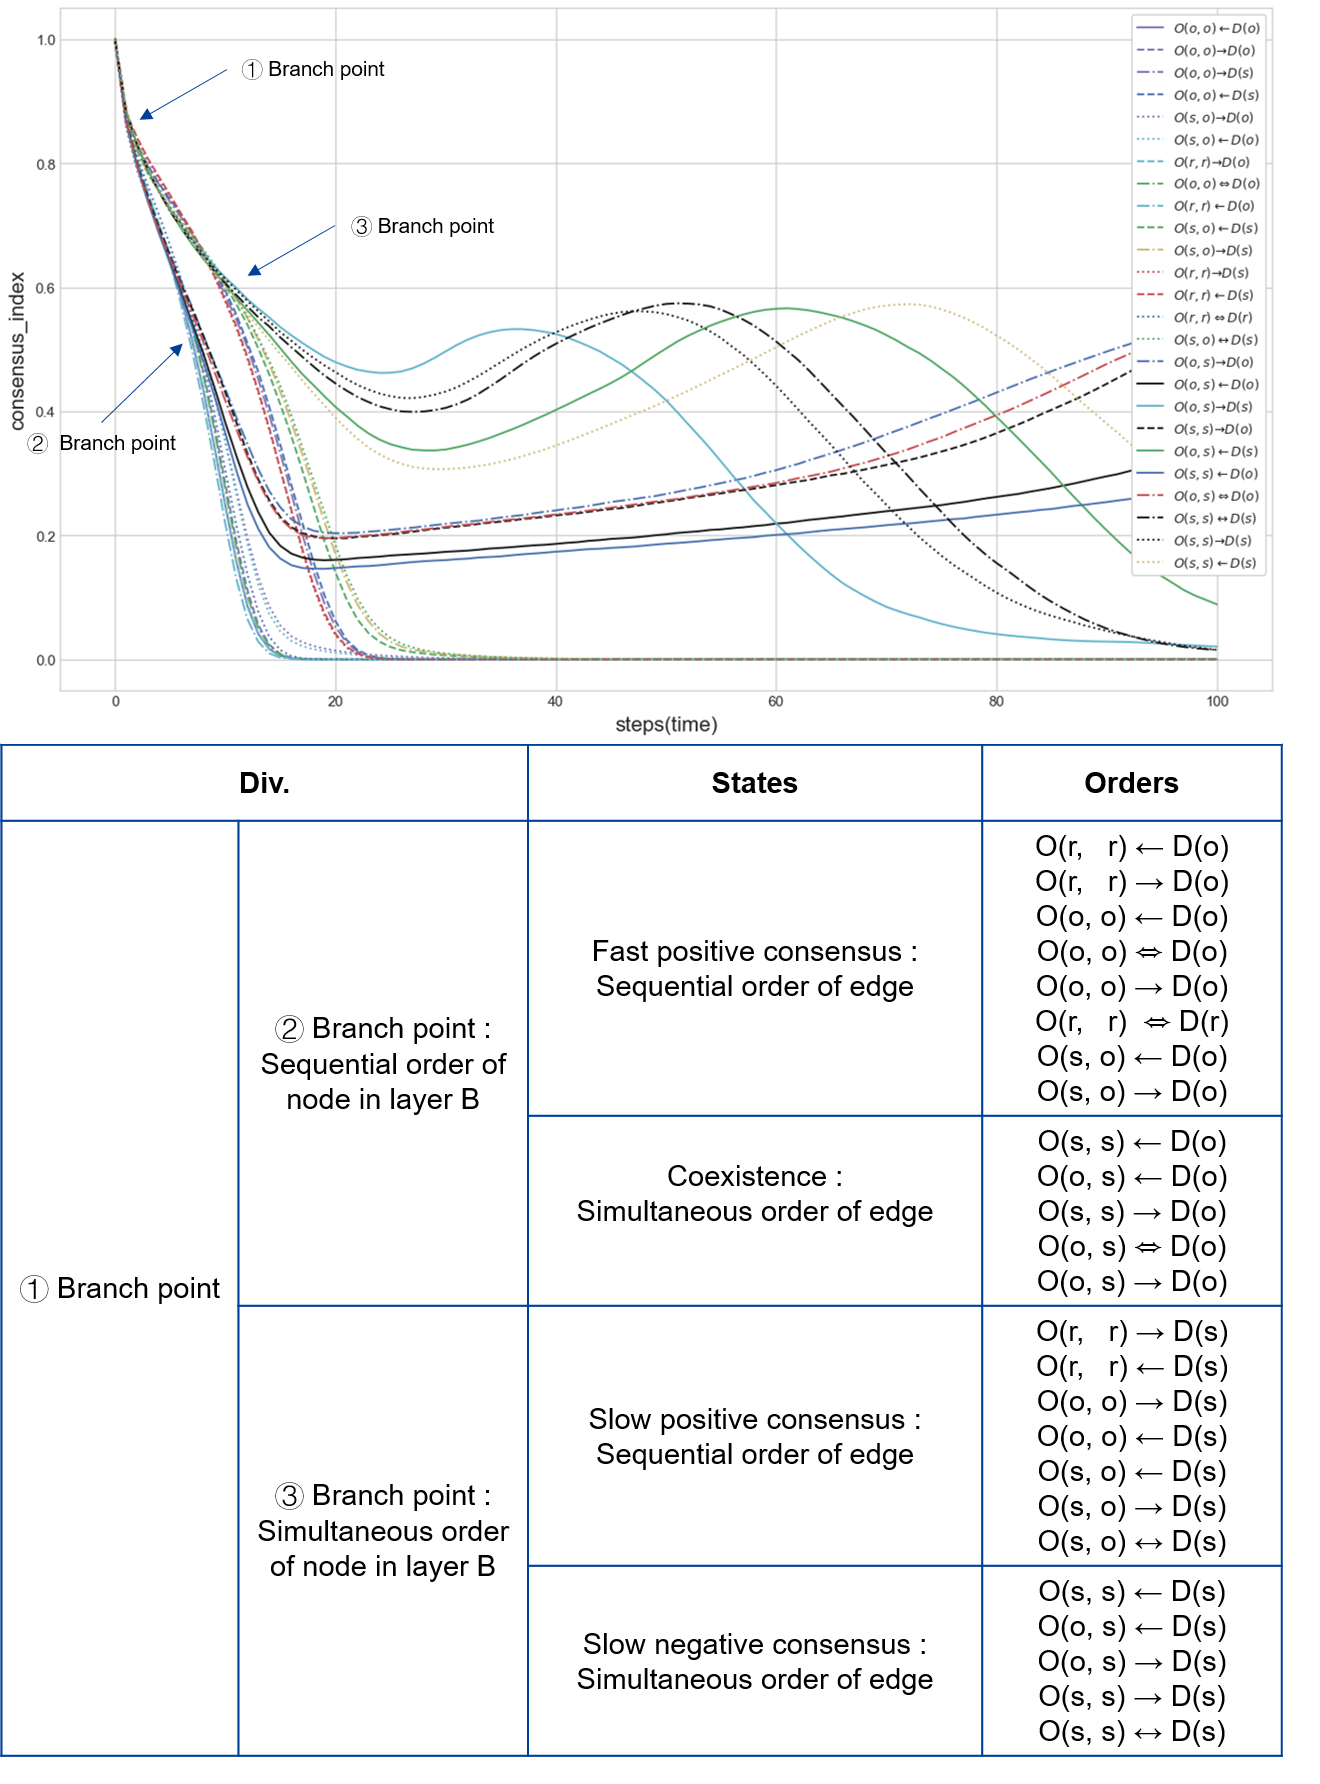
\includegraphics[width=\hsize]{figure/chap4_ordertotal2.png}
	\caption{Total results of 25 updating rules with \textit{CI}}
	\label{ordertotal2}
\end{figure}


\section{Conclusion}
Through these results, several important facts could be arranged. First, networks with simultaneous updating rules tend to make slow consensus or coexistence, sometimes make transition to opposite orientation. On the other hands, networks with sequential updating rules have a tendency to make fast consensus. Second, dynamics order between layers does not have an influence for network state, though there exists tiny consensus time gap. Third, order of nodes in layer B has more influence for network states than order of nodes in layer A because order of nodes in layer B makes the first branch point that has a vital role to make fast or slow convergent. That means the communication method in decision making layer is very important for determining consensus time. Fourth, order of edges in layer A is very influential so that it makes the second and third branch points that determine the final state of network. It can be analyzed as that characteristics of nodes in layer A, such as rash and considerate, has same orientation consensus or make transition to coexistence or opposite orientation consensus.




%# -*- coding: utf-8-unix -*-
% !TEX program = xelatex
% !TEX root = ../thesis.tex
% !TEX encoding = UTF-8 Unicode
%%==================================================
%% chapter02.tex for SJTU Master Thesis
%% based on CASthesis
%% modified by wei.jianwen@gmail.com
%% Encoding: UTF-8
%%==================================================

\chapter{Influences of key nodes on competition}
\label{chap5}
In this chapter, it is investigated which nodes have the most important influence for keeping or changing their orientation on a two-layer network. There exist many methods to select key nodes, such as Pagerank, degree centrality, eigenvector centrality, betweenness centrality, and closeness centrality. Moreover, in \parencite{mesgari2015, huang2014}, it has been proved that multiple indicators that use the rank difference of several node centralities are useful to identify key nodes and prevent the slow way to identify critical nodes. Based on these methods, such as single-node centrality(single indicators) and combined node centrality(multiple indicators), it is researched which method is the most effective and the most influential for selecting key nodes.  

\section{Method for selecting key nodes}
\label{sec:method for finding key nodes}
As the initial conditions for selecting key nodes, each layer is made of a \textit{BA} network with $512$ nodes, $K=3$, and $1$ external edge. Each simulation takes $100$ steps for opinion evolution, and $100$ simulations are considered for average results. In order to demonstrate the influence of key nodes, the parameters such as $p$ and $v$ are set to be the opposite consensus state to the initial state of a layer for identifying key nodes. And then the stubborn nodes that do not change their states during the opinion evolution are selected by using methods for selecting key nodes, and the ratio of stubborn nodes is increased until a state of the network is changed into the same consensus state with the initial state of the layer for identifying key nodes. Under these conditions, the most powerful method is the fastest method to reach the same consensus state with the initial state of a layer for selecting key nodes. For example, for selecting key nodes on layer A(positive opinion), the parameters are set to be a negative consensus state. Then, as the stubborn nodes on layer A are selected by node centrality or other methods, and the ratio of the stubborn nodes is increased, a state of the network is gradually changed into a positive state. Inversely for selecting key nodes on layer B(negative opinion), the parameters are set to be a positive consensus state. Then, as the stubborn nodes on layer B are selected by the method for recognizing key nodes, and the ratio of stubborn nodes is increased, a state of the network is gradually changed into a negative state. Here, we find the fastest and most powerful method.

As the method to select stubborn nodes, we use two kinds of indicators, single indicators, and multiple indicators. As single indicators, node centralities are applied, such as Pagerank, degree, eigenvector, closeness, and betweenness. As multiple indicators, combined node centralities that consist of several node centralities are applied.
  
First, here is the way to select key nodes by using a single node centrality.
\begin{enumerate}
	\item All nodes are ranked by five node centralities(Pagerank, degree, eigenvector, closeness, betweenness).
	\item The nodes are deactivated from high ranked order until the state of network has a significant difference, i.e., the stubborn nodes are selected according to high ranked order, and the ratio of stubborn nodes is increased. 
	\item The results are compared according to node centralities. When a node centrality makes the state of network reach the fastest to the opposite consensus state with the initial condition or have the most significant change, it is the most powerful method for selecting key nodes.
	\item As the ratio of stubborn nodes is increased, the summation of $AS$, which represents the `Average States' of a network, is calculated on every single indicator. It is recognized that the larger the $AS$ value is on layer A, the more influential that indicator is, inversely the smaller the $AS$ value is on layer B, the more influential that indicator is.
\end{enumerate}

Furthermore, we research the way to recognize critical nodes by using multiple indicators such as combined node centralities(\textit{PR+DE, PR+BE, DE+BE, PR+DE+BE}). Combined node centralities are made up of several selected node centralities. When it is proven that a node centrality is useful for selecting key nodes through the simulations, it is selected as a factor of combined node centrality. Here, $2$ or $3$ node centralities are selected, such as Pagerank, degree, and betweenness. 
The way to recognize key nodes by using combined node centrality follows like this steps. 
\begin{enumerate}
	\item  Each selected node centrality ranks all nodes. All nodes have the ranks as the number of selected node centralities.  
	\item Combined node centrality is calculated by the summation of all ranks which a node has. 
	\item All nodes are ranked again by combined node centrality. The smaller the combined node centrality is, the higher a node is ranked.        
	\item The nodes are deactivated from high ranked order until the state of network has a significant difference, i.e., the stubborn nodes are selected according to high ranked order, and the ratio of stubborn nodes is increased. 
\end{enumerate}

It has been already proven that a single node centrality has good performance to identify key nodes.\parencite{koschutzki2008, francisco2019, bianconi2018}. However, identifying key nodes by multiple indicators is still an open problem because there are lots of ways to set up and optimize the weight of each node centrality.\parencite{huang2014}  Here, we simplify the method by setting the weights as equal and calculate the summation of ranks. Although our multiple indicators need to be researched further, the multiple indicators are evaluated and compared with single indicators. The method for measuring and evaluating key nodes on \textit{BA-BA} network follows as \ref{layerA} and \ref{layerB}.\\
 
\subsection{Key nodes on layer A}
\label{layerA}
\begin{figure}[!htb]
	\centering
	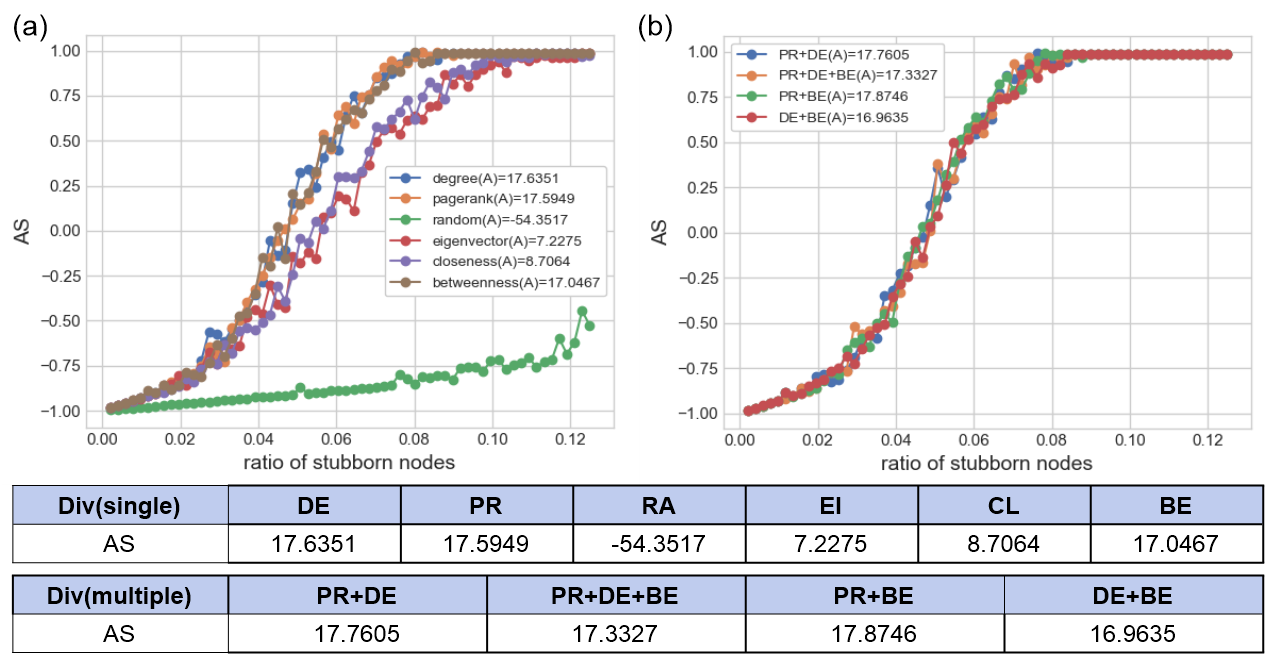
\includegraphics[width=\hsize]{figure/chap5_keynode_A.png}
	\caption{Key nodes on layer A in \textit{BA(3)-BA(3)} network($p=0.2, v=0.4$): (a) Single indicator methods, (b) Multiple indicator methods}
	\label{chap5_keynode_A}
\end{figure}
To select key nodes on layer A, parameters are set to be negative consensus state like $p=0.2, v=0.4$.  As single indicators, five node centralities(Pagerank, degree, eigenvector, closeness, betweenness) are used, and the influence of randomly selected nodes is also compared with five node centralities. As multiple indicators, $2$ or $3$ node centralities are combined, such as Pagerank, degree, and betweenness, which have good performance as single indicators. In combined node centralities, we denote Pagerank, degree, and betweenness as \textit{PR, DE, BE}. Moreover, when they are combined, the methods are denoted as \textit{PR+DE, PR+BE, DE+BE, PR+DE+BE} by using \textit{+}. 

Fig.~\ref{chap5_keynode_A} shows the simulation result for recognizing key nodes on layer A. As a single indicator, Pagerank has the best performance. The next ranks are degree and betweenness. As multiple indicators, \textit{PR+BE} has the most effective result. The next is \textit{PR+DE}. These two methods of multiple indicators work better than Pagerank. Compared with all methods, the best method is \textit{PR+BE}. It can be found out that some multiple indicators are more useful for selecting key nodes than single indicators. \\

\subsection{Key nodes on layer B}
\label{layerB}
\begin{figure}[!htb]
	\centering
	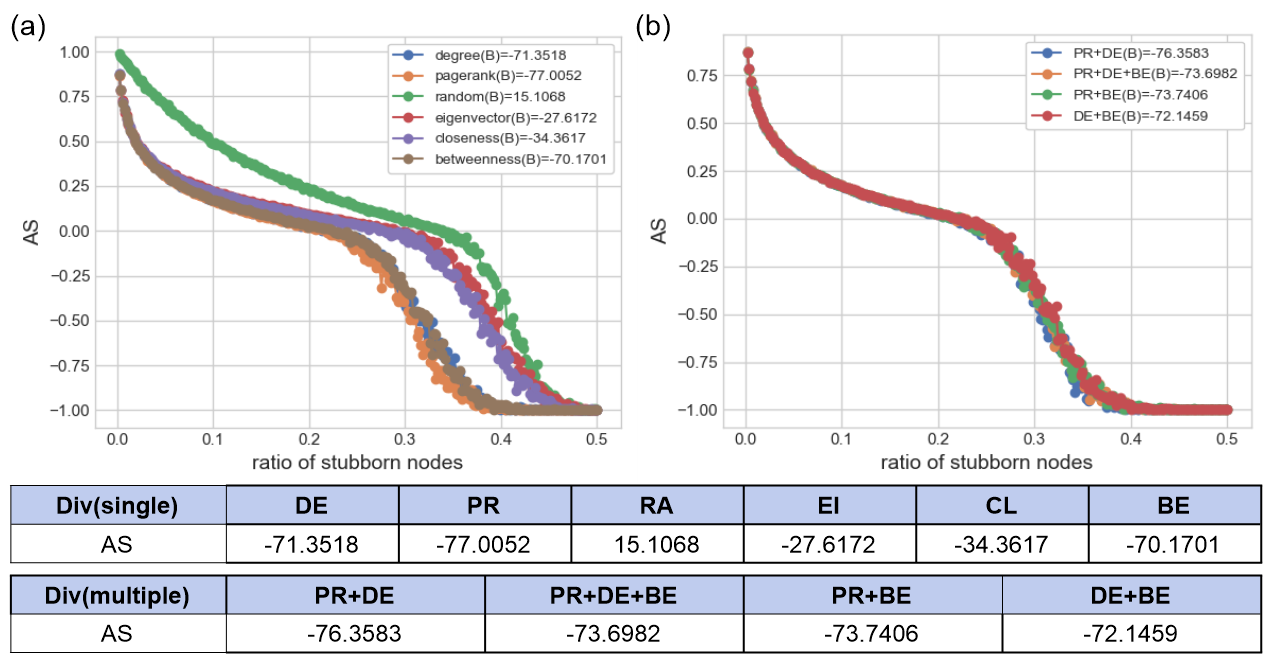
\includegraphics[width=\hsize]{figure/chap5_keynode_B.png}
	\caption{Key nodes on layer B in \textit{BA(3)-BA(3)} network($p=0.3, v=0.5$): (a) Single indicator methods, (b) Multiple indicator methods}
	\label{chap5_keynode_B}
\end{figure}

To select key nodes on layer B, parameters are set to be positive consensus state such as $p=0.3, v=0.5$. Fig.~\ref{chap5_keynode_B} shows the simulation result for identifying key nodes on layer B. As a single indicator, the most effective way to recognize important nodes is Pagerank centrality. The next ranks are degree and betweenness. As multiple indicators, \textit{PR+DE} has the best performance. Pagerank is the most effective method for selecting key nodes on layer B. But, all multiple indicators work better than degree centrality, the second rank in single indicators. It can be found out that combined node centralities also have a good performance for selecting key nodes, though they are not the best. \\

\section{Key nodes on two-layer networks with different structures}
In this section, we select the key nodes in the networks with various structures that are described in the chapter~\ref{chap3}. Node centralities and combined node centralities are also used as the methods for selecting key nodes. First, \textit{Hierarchical Model} is applied to identify critical nodes. Second, we consider the case that each layer has a different network type, such as \textit{BA-RR} or \textit{RR-BA} networks. Third, the case is considered that each layer has a different number of internal edges. Layer A can have more internal links, or layer B can have more internal links. Both cases are simulated. \\

\subsection{Key nodes in Hierarchical Model}
\begin{figure}[!htb]
	\centering
	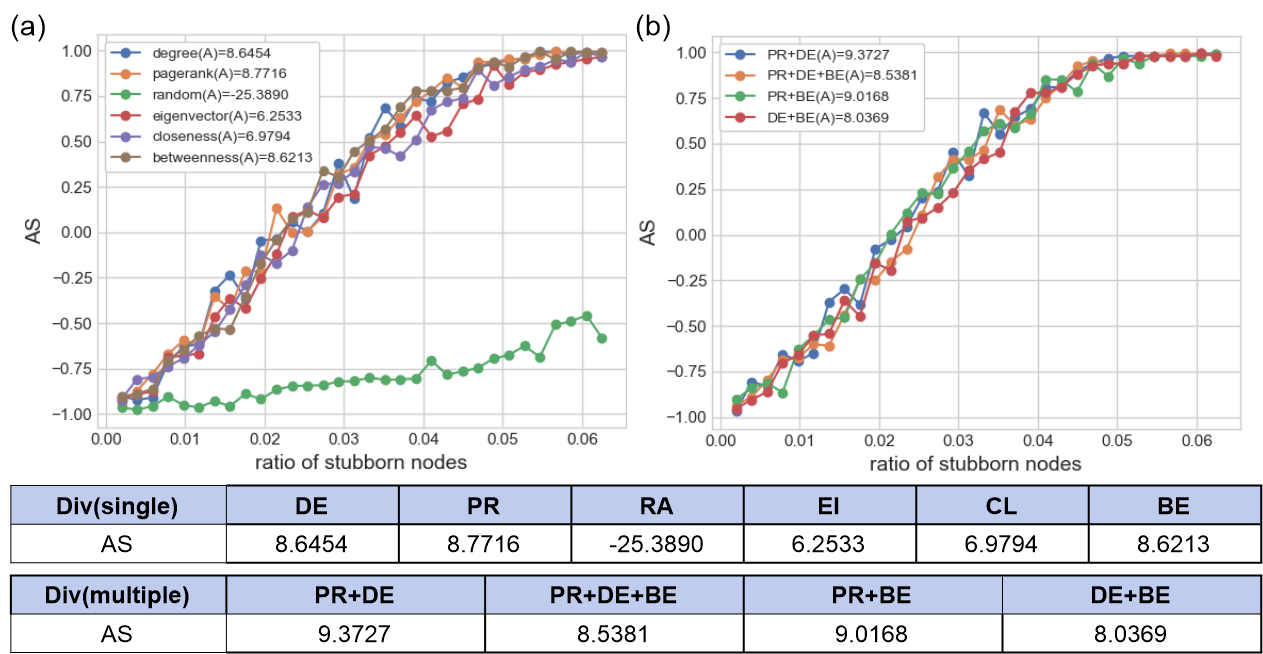
\includegraphics[width=\hsize]{figure/chap5_keynode_HM_A.png}
	\caption{Key nodes on layer A in \textit{Hierarchical Model(8)}($p=0.2, v=0.2$):
		(a) Single indicator methods, (b) Multiple indicator methods}
	\label{chap5_keynode_HM_A}
\end{figure}
\begin{figure}[!htb]
	\centering
	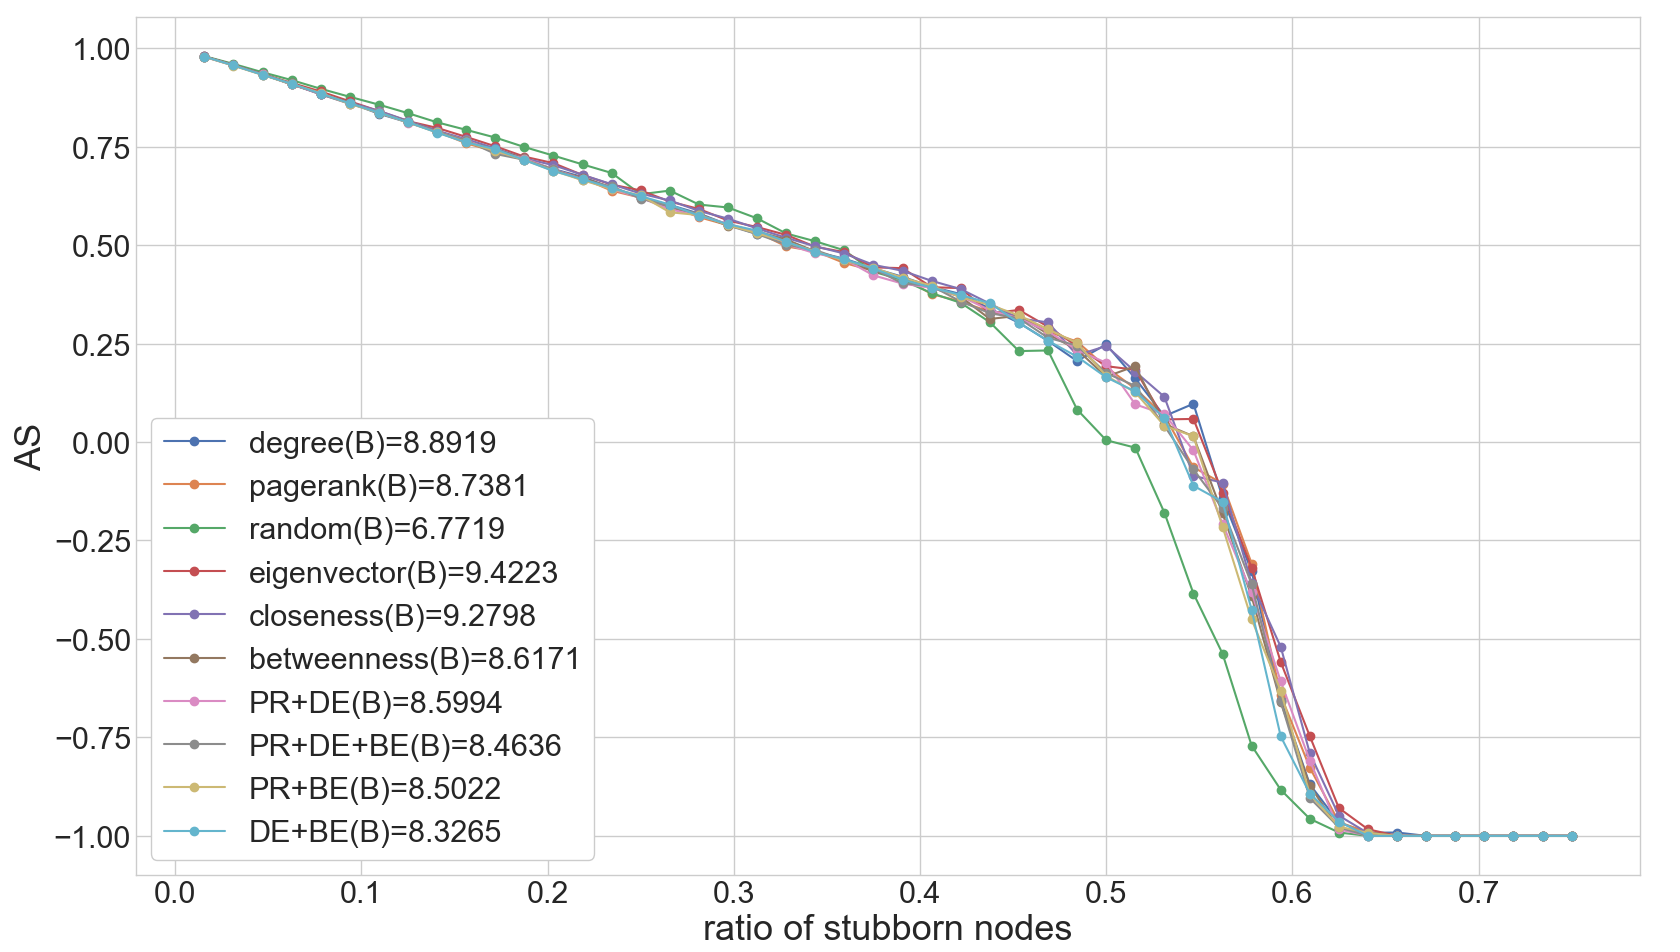
\includegraphics[width=\hsize]{figure/chap5_keynode_HM_B.png}
	\caption{Key nodes on layer B in \textit{Hierarchical Model(8)}($p=0.25, v=0.3$):
		(a) Single indicator methods, (b) Multiple indicator methods}
	\label{chap5_keynode_HM_B}
\end{figure}

As described in the chapter~\ref{chap3}, \textit{Hierarchical Model} is the two-layer network that the number of nodes in layer B is reduced at a specific rate, and the external links from nodes in layer B are increased accordingly. Here, each layer consists of a \textit{BA} network with $k=3$. Layer A has $512$ nodes, and layer B has $64$ nodes. We denote this model as \textit{HM(8) with BA(3)}.

Fig.~\ref{chap5_keynode_HM_A} shows the simulation result of key nodes on layer A. Simulation result represents that \textit{PR+DE} is the best method for recognizing key nodes on \textit{HM(8) with BA(3)}. The next ranks are \textit{PR+BE} and Pagerank. The curve of changing the network states shown in Fig.~\ref{chap5_keynode_HM_A} is more straight than Fig.~\ref{chap5_keynode_A}. That means the speed of changing network states(consensus time) is much faster. 

Fig.~\ref{chap5_keynode_HM_B} shows the simulation result of key nodes on layer B. However, the result is different from other simulation results. The best performance method is a random method. That means node centralities do not work on this model. Furthermore, the curve of changing the network states shown in Fig.~\ref{chap5_keynode_HM_B} is also more straight than Fig.~\ref{chap5_keynode_B}, which means the consensus is much easier, and the consensus time is much shorter. It is found out that the \textit{Hierarchical Model} makes it hard to recognize key nodes on layer B and make it easy to reach a consensus of two-layer by key nodes. \\

\subsection{Key nodes on the two-layer network with different network types}
Here, we consider two types of networks, \textit{BA-RR} and \textit{RR-BA}. The number of internal links on each layer is set up as the same or almost the same number to exclude the influence of internal degrees. These models are compared with the \textit{BA-BA} to find out the influence of network types under the same conditions, such as $p$, $v$, and $the ratio of stubborn nodes$.  

\begin{figure}[!htb]
	\centering
	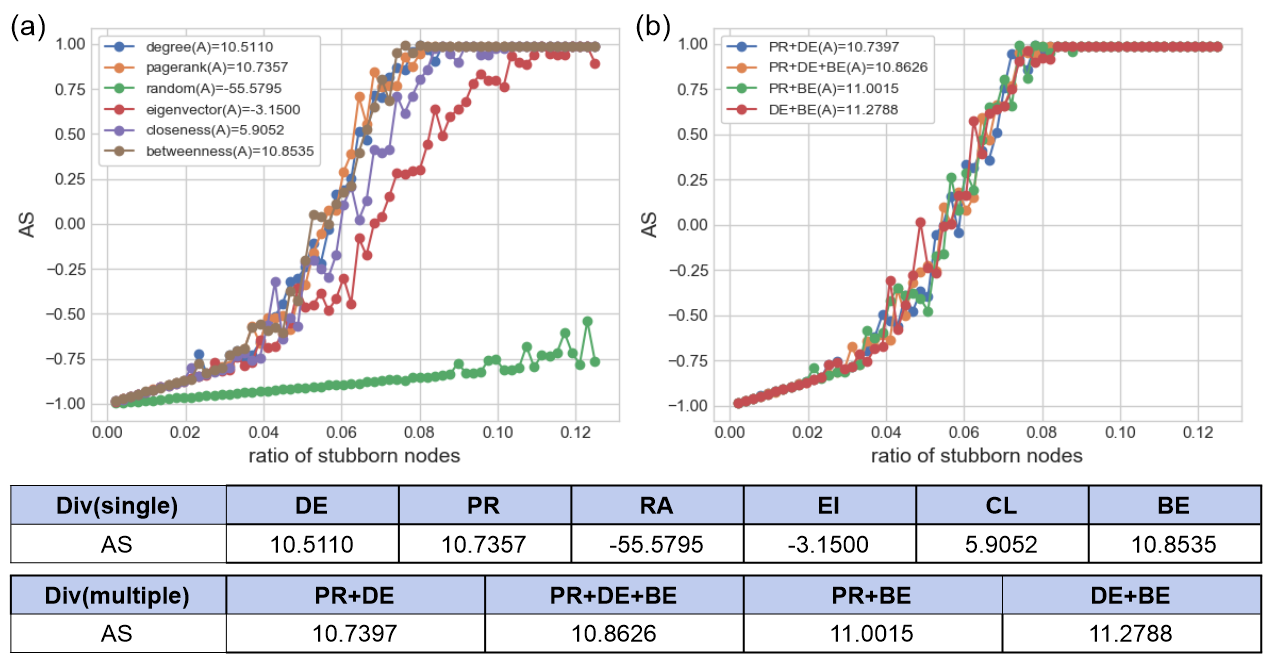
\includegraphics[width=\hsize]{figure/chap5_keynode_BA_RR_A.png}
	\caption{Key nodes on layer A in \textit{BA(3)-RR(6)} network($p=0.2, v=0.4$):
		(a) Single indicator methods, (b) Multiple indicator methods}
	\label{chap5_keynode_BA_RR_A}
\end{figure}
\begin{figure}[!htb]
	\centering
	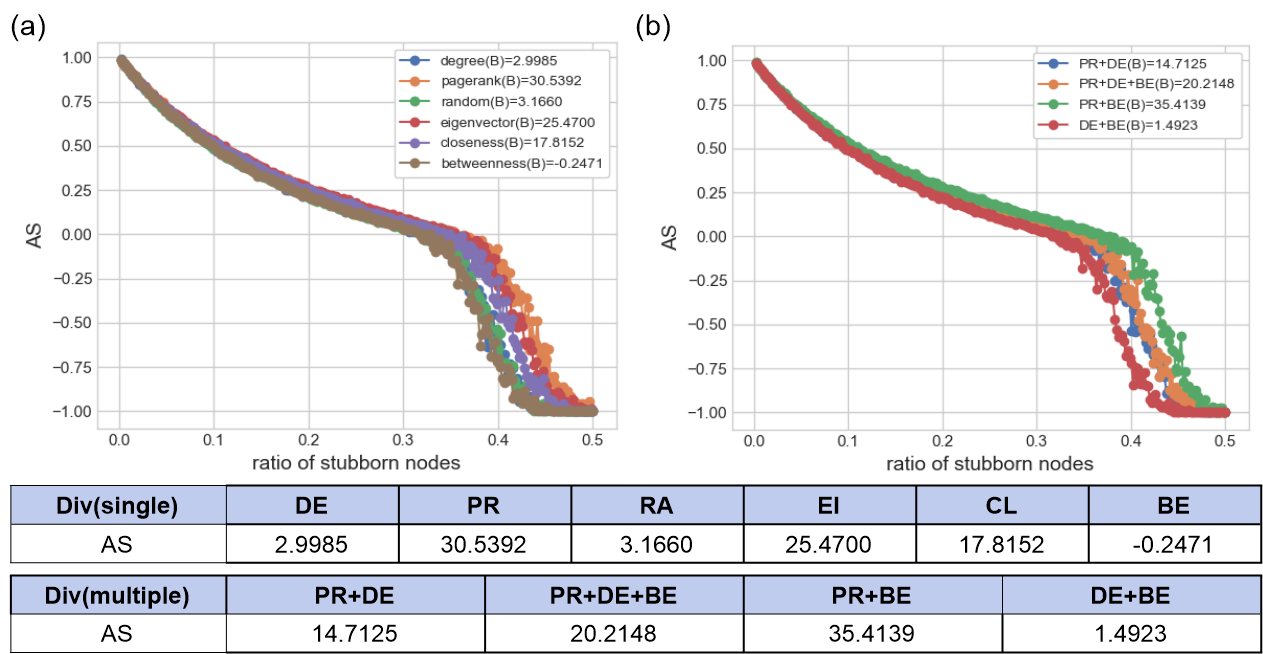
\includegraphics[width=\hsize]{figure/chap5_keynode_BA_RR_B.png}
	\caption{Key nodes on layer B in \textit{BA(3)-RR(6)} network($p=0.3, v=0.5$):
		(a) Single indicator methods, (b) Multiple indicator methods}
	\label{chap5_keynode_BA_RR_B}
\end{figure}

First, the \textit{BA-RR} network is investigated. Fig.~\ref{chap5_keynode_BA_RR_A} shows the simulation result of key nodes on layer A.\textit{PR+BE} is the most powerful method. The next rank is Pagerank as a single indicator. Compared with the \textit{BA(3)-BA(3)} shown in Fig.~\ref{chap5_keynode_A}, \textit{BA(3)-RR(6)} has smaller \textit{AS} values and a more gentle curve to change the state of the network. 

Fig.~\ref{chap5_keynode_BA_RR_B} shows the simulation result of key nodes on layer B. Betweenness is the best method for identifying key nodes on layer B in the \textit{BA-RR} network. In this model, the degree centrality is not an exact method for the selection of key nodes because the degree of each node is the same in the \textit{RR} network. However, random and degree method is the third and fourth method for recognizing key nodes. That means other methods except for betweenness do not work for identifying key nodes. Compared with the \textit{BA(3)-BA(3)} shown in Fig.~\ref{chap5_keynode_B}, the \textit{BA(3)-RR(6)} has more massive \textit{AS} values and a more gentle curve to change the state of the network. 

\begin{figure}[!htb]
	\centering
	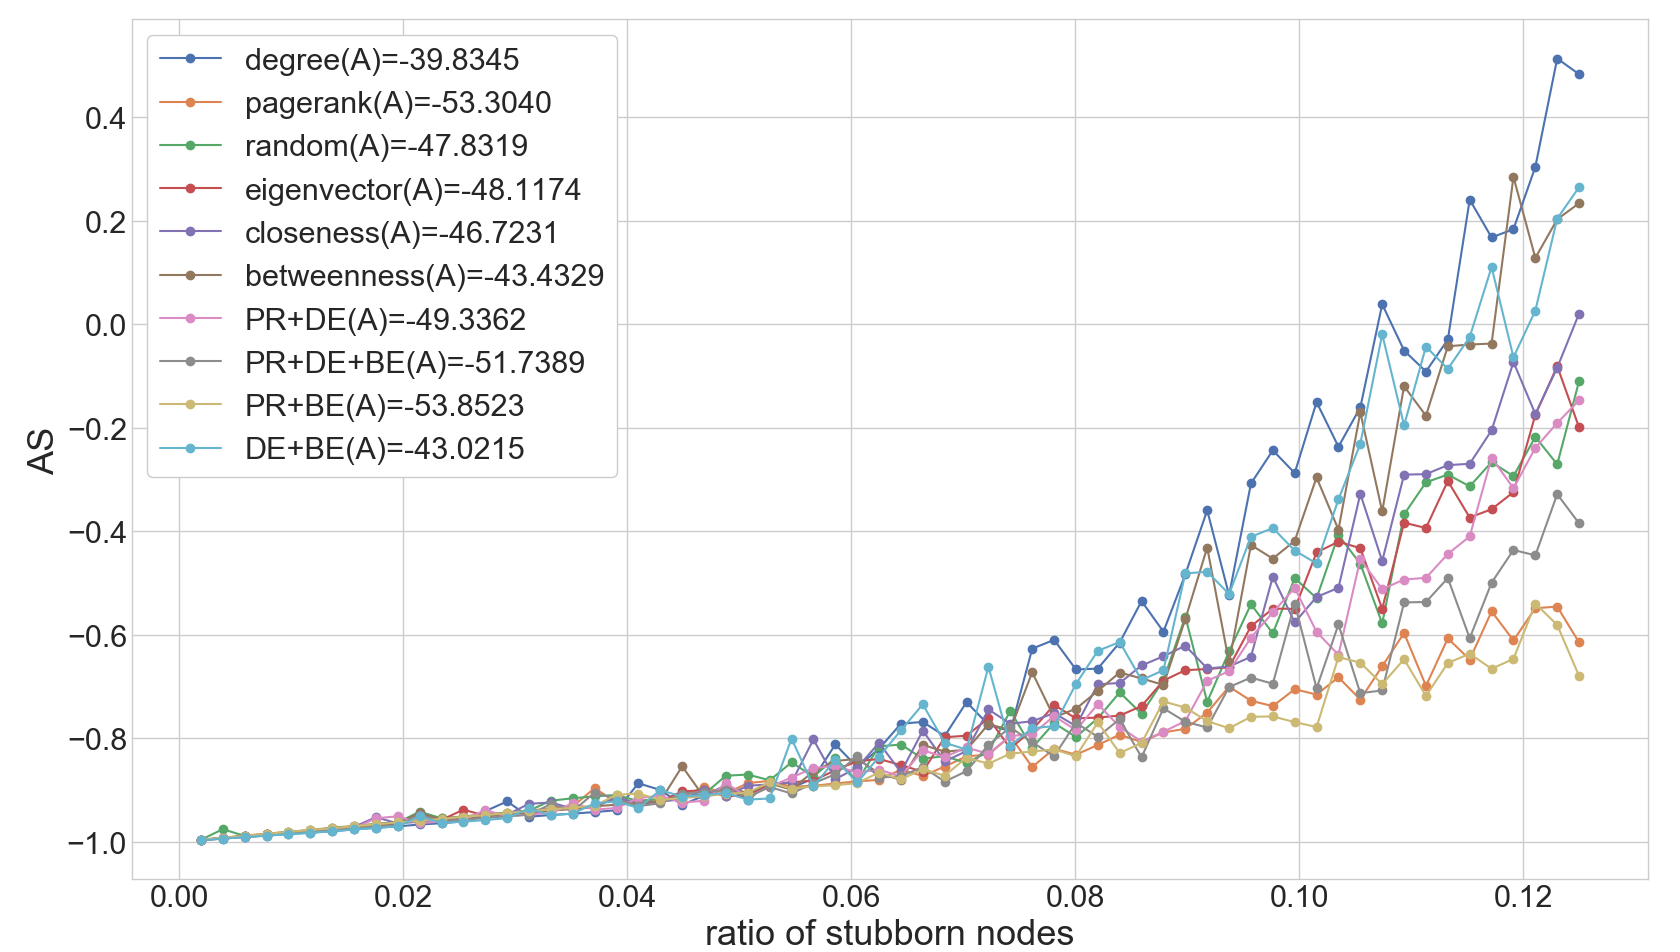
\includegraphics[width=\hsize]{figure/chap5_keynode_RR_BA_A.png}
	\caption{Key nodes on layer A in \textit{RR(6)-BA(3)} network($p=0.2, v=0.4$):
		(a) Single indicator methods, (b) Multiple indicator methods}
	\label{chap5_keynode_RR_BA_A}
\end{figure}
\begin{figure}[!htb]
	\centering
	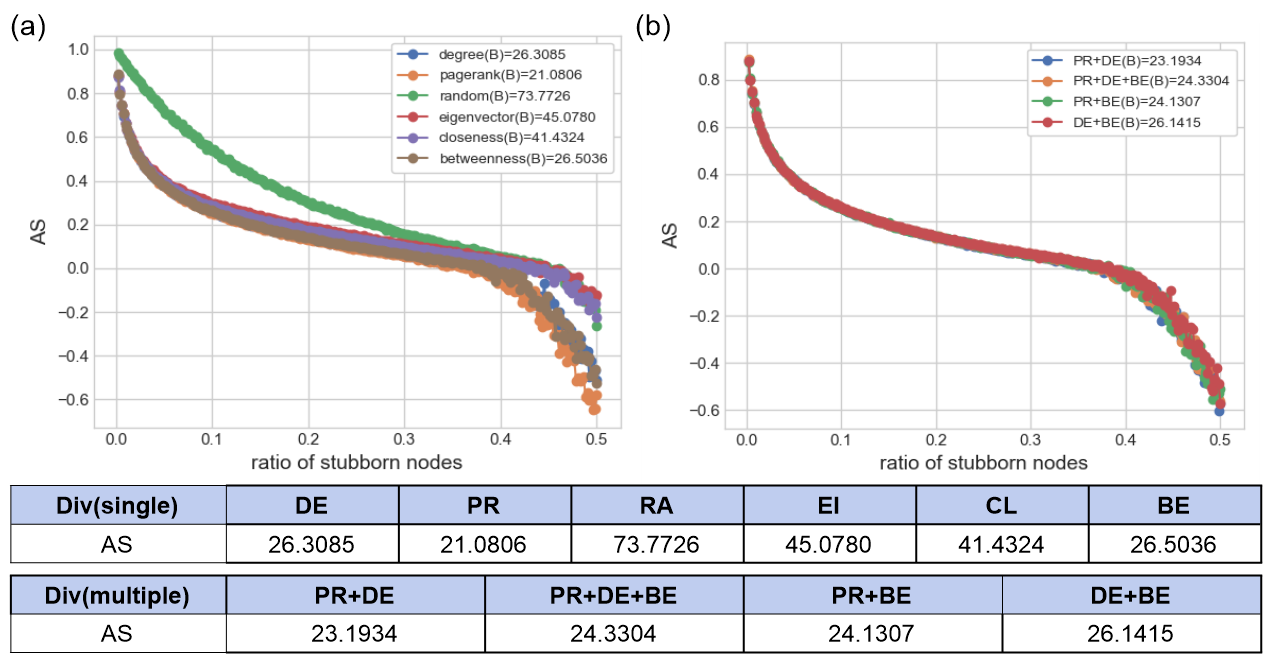
\includegraphics[width=\hsize]{figure/chap5_keynode_RR_BA_B.png}
	\caption{Key nodes on layer B in \textit{RR(6)-BA(3)} network($p=0.3, v=0.5$):
		(a) Single indicator methods, (b) Multiple indicator methods}
	\label{chap5_keynode_RR_BA_B}
\end{figure}

Next, the \textit{RR-BA} network is considered. Fig.~\ref{chap5_keynode_RR_BA_A} shows the simulation result of key nodes on layer A. The best method is degree centrality. However, in this model, degree centrality is not meant for recognizing key nodes because all nodes in layer A have the same degree. Here, the reason why degree centrality has excellent performance is analyzed as those dynamics are very efficient because nodes are sequentially changed into the stubborn node and interacted(when nodes have the same node centrality, nodes are changed into stubborn nodes sequentially according to interaction order under given algorithm). Moreover, other single indicators have similar \textit{AS} values with the random method. That means node centralities do not work for identifying key nodes though betweenness has better performance than other methods. Compared with the \textit{BA(3)-BA(3)} shown in Fig.~\ref{chap5_keynode_A}, \textit{RR(6)-BA(3)} has smaller \textit{AS} values and does not reach the opposite consensus yet. 

Fig.~\ref{chap5_keynode_RR_BA_B} shows the simulation result of key nodes on layer B. Pagerank has the best performance. The next rank is \textit{PR+DE}.  Compared with the \textit{BA(3)-BA(3)} shown in Fig.~\ref{chap5_keynode_B} , the \textit{RR(6)-BA(3)} has more massive \textit{AS} values and a more gentle curve to change the state of the network. 

Compared with the \textit{BA-BA} network, both \textit{BA-RR} and \textit{RR-BA} have a more gentle curve line to change the state of the network. It can be analyzed that the \textit{RR} network makes it slow for crucial nodes to change the state of the network and makes it hard to select critical nodes though betweenness has excellent performance on the \textit{RR} network.\\  

\subsection{Key nodes on the two-layer network with different number of internal links}
Next, the case is considered that each layer has a different number of internal edges. In case that layer A has a more massive number of internal links, layer A consists of a \textit{BA} network with $k=4$, but layer B consists of a \textit{BA} network with $k=2$. Inversely, in case that layer B has a more massive number of internal links, layer B consists of a \textit{BA} network with $k=4$, but layer A consists of a \textit{BA} network with $k=2$. 

\begin{figure}[!htb]
	\centering
	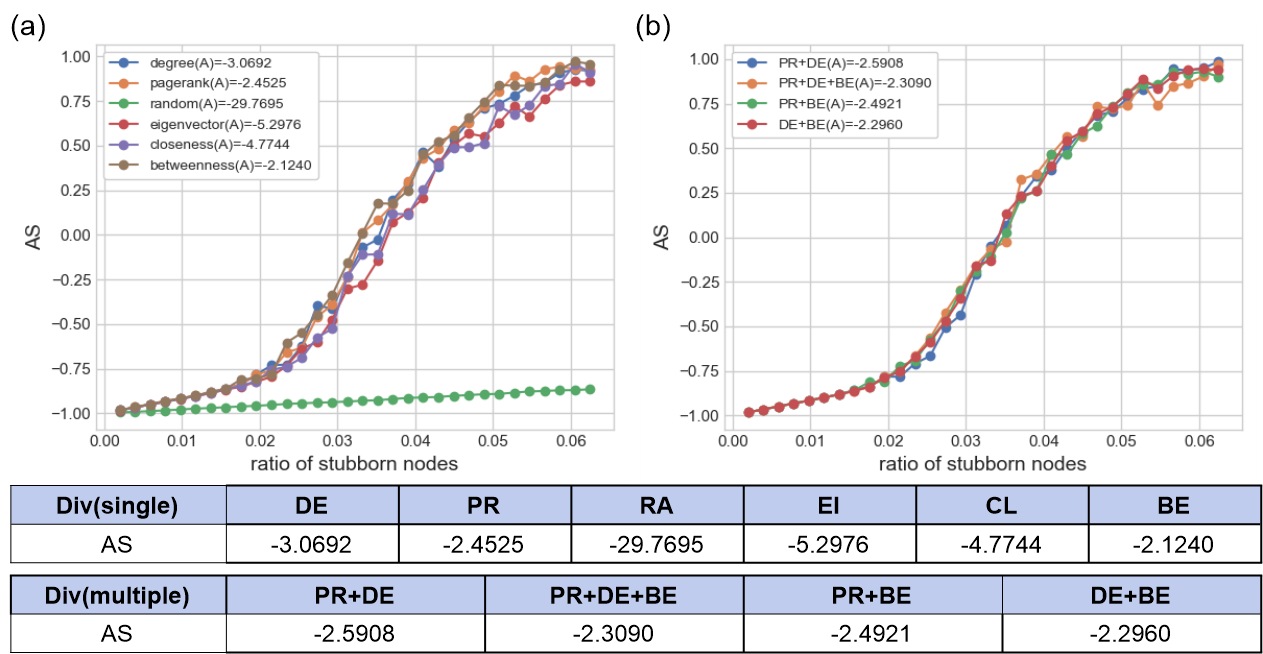
\includegraphics[width=\hsize]{figure/chap5_keynode_internal_A.png}
	\caption{Key nodes on layer A in \textit{BA(4)-BA(2)} network($p=0.15, v=0.3$):
		(a) Single indicator methods, (b) Multiple indicator methods}
	\label{chap5_keynode_internal_A}
\end{figure}
\begin{figure}[!htb]
	\centering
	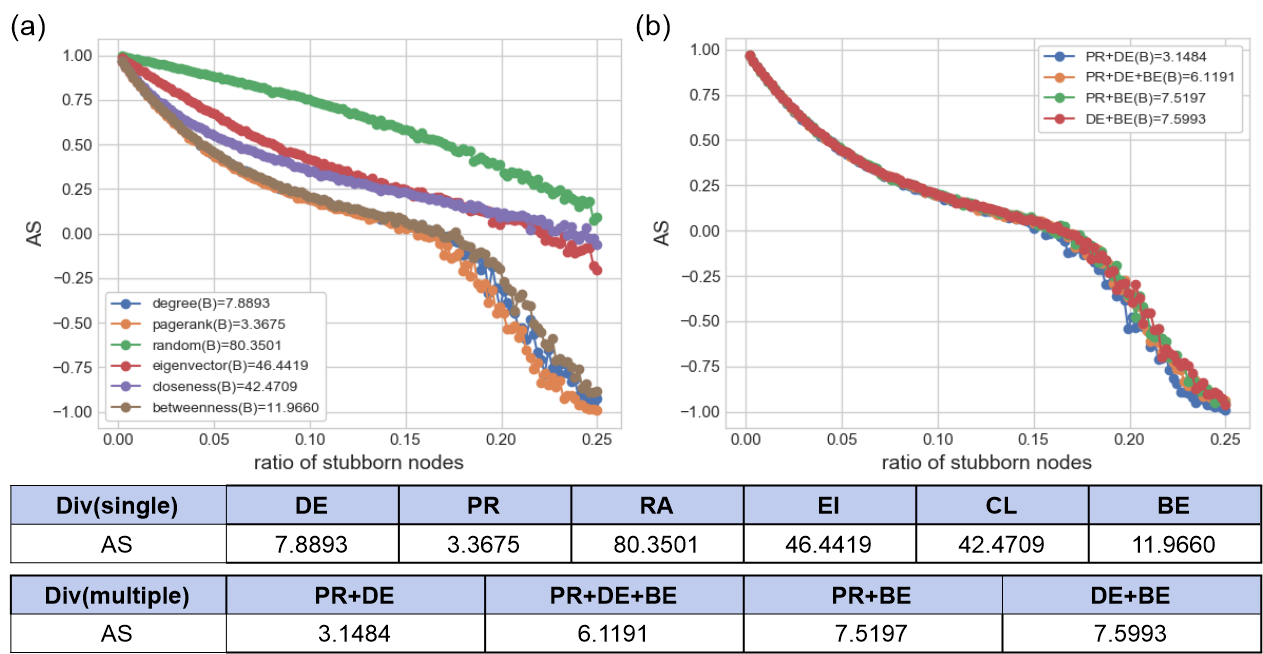
\includegraphics[width=\hsize]{figure/chap5_keynode_internal_B.png}
	\caption{Key nodes on layer B in \textit{BA(4)-BA(2)} network($p=0.2, v=0.4$):
		(a) Single indicator methods, (b) Multiple indicator methods}
	\label{chap5_keynode_internal_B}
\end{figure}

First, the case of more internal links on layer A than layer B is investigated. Fig.~\ref{chap5_keynode_internal_A} shows the simulation result of key nodes on layer A in the \textit{BA(4)-BA(2)} network. Betweenness has the best performance for selecting key nodes. The next ranks are \textit{DE+BE}, \textit{PR+BE}, and \textit{PR+DE+BE}. Compared with the \textit{BA(2)-BA(4)} network shown in Fig.~\ref{chap5_keynode_internal_A2}, the curve of changing the state that is shown in Fig.~\ref{chap5_keynode_internal_A} is much more straight-line. That means consensus time is short, and it is easy to have consensus.

Fig.~\ref{chap5_keynode_internal_B} shows the simulation result of key nodes on layer B in the \textit{BA(4)-BA(2)} network. \textit{PR+DE} is the most powerful method. The next ranks are Pagerank, \textit{PR+DE+BE}, and \textit{PR+BE}. Compared with the \textit{BA(2)-BA(4)} network shown in Fig.~\ref{chap5_keynode_internal_B2}, the curve of changing the state that is shown in Fig.~\ref{chap5_keynode_internal_B} is also more straight-line. 

Compared with the \textit{BA(2)-BA(4)} network, it can be analyzed that more internal edges on layer A make it easy to have a consensus by key nodes. 

\begin{figure}[!htb]
	\centering
	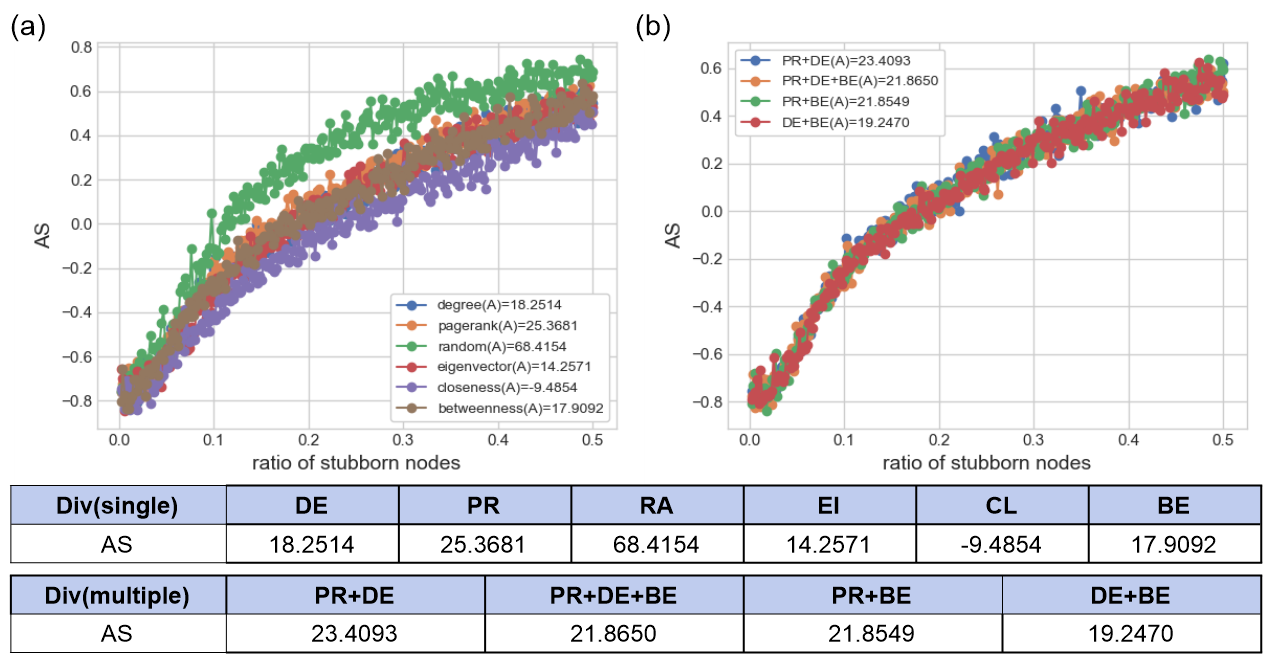
\includegraphics[width=\hsize]{figure/chap5_keynode_internal_A2.png}
	\caption{Key nodes on layer A in \textit{BA(2)-BA(4)} network($p=0.57, v=0.37$):
		(a) Single indicator methods, (b) Multiple indicator methods}
	\label{chap5_keynode_internal_A2}
\end{figure}
\begin{figure}[!htb]
	\centering
	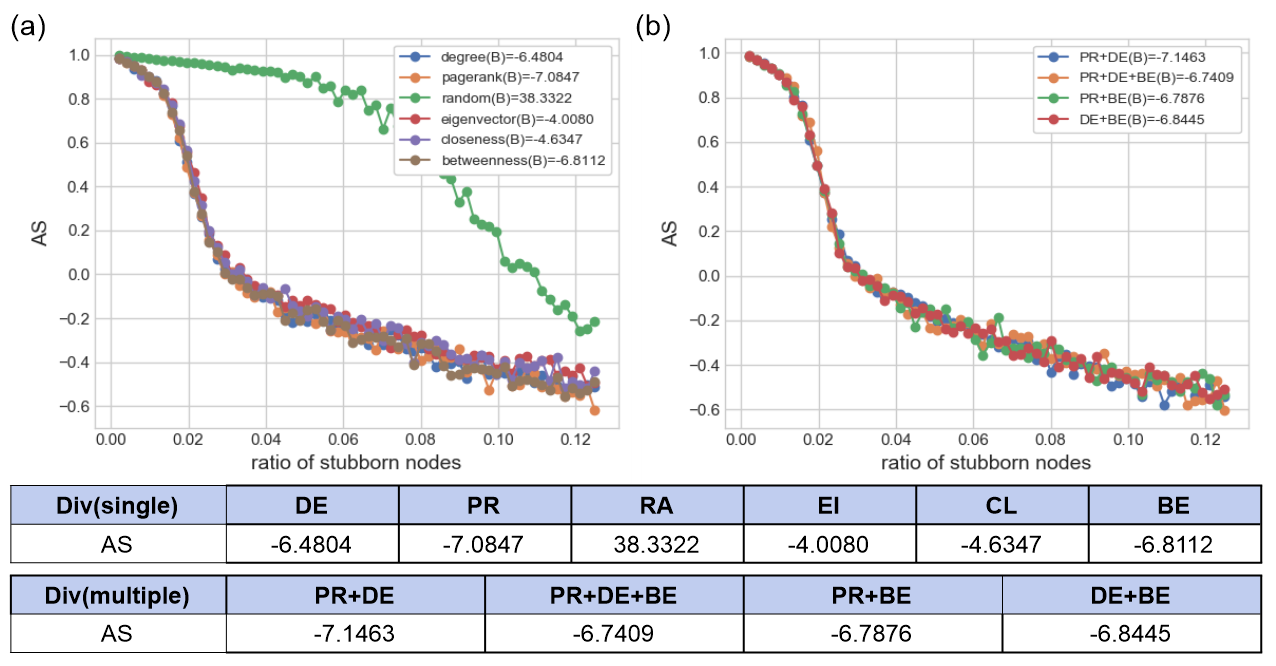
\includegraphics[width=\hsize]{figure/chap5_keynode_internal_B2.png}
	\caption{Key nodes on layer B in \textit{BA(2)-BA(4)} network($p=0.6, v=0.4$):
		(a) Single indicator methods, (b) Multiple indicator methods}
	\label{chap5_keynode_internal_B2}
\end{figure}

Next, the case of more internal links on layer B than layer A is researched. Fig.~\ref{chap5_keynode_internal_A2} shows the simulation result of key nodes on layer A in the \textit{BA(2)-BA(4)} network. However, the simulation results are different from other results because the random method has the best performance. That means node centralities do not work on this model. Compared with the \textit{BA(4)-BA(2)} network shown in Fig.~\ref{chap5_keynode_internal_A}, the curve of changing the state that is shown in Fig.~\ref{chap5_keynode_internal_A2}  is much slower and more gentle.

Fig.~\ref{chap5_keynode_internal_B2} shows the simulation result of key nodes on layer B in the \textit{BA(2)-BA(4)} network. \textit{PR+DE} has the most effective performance. The next ranks are Pagerank, \textit{DE+BE}, and betweenness. Compared with the \textit{BA(4)-BA(2)} network shown in Fig.~\ref{chap5_keynode_internal_B}, the curve of changing the state that is shown in Fig.~\ref{chap5_keynode_internal_B2} is much faster at the beginning but much slower at the end. Besides, consensus does not happen in this model.

Compared with the \textit{BA(4)-BA(2)} network, it can be analyzed that the larger number of internal edges on layer B makes consensus by key nodes hard. Moreover, decreasing internal edges on layer A makes it hard to select key nodes on layer A.\\   

\section{Conclusion}
By using node centrality and combined node centrality, key nodes on each layer have been recognized on networks with various structures. Table~\ref{effective methods} shows total simulation results for selecting key nodes on various interconnected networks.
 
\begin{table}[!htb]
	\scriptsize
	\centering
	\caption{Effective method for selecting key nodes on various networks}
	\label{effective methods}
	\begin{center}
		\begin{tabular}{c|c|c|c|c|c|c|c|c|c} \hline\hline
		  Div                              & A nodes & B nodes & A edges & B edges & layer & 1st method & 2nd method  & 3rd method  & remarks    \\ \hline \hline
         \multirow{1}{*}{BA(3)-BA(3)}      & 512 	 & 512     & 1,527   & 1,527   & A     & PR+BE      & PR+DE       & Pagerank    &            \\ 
			                               &  	     &         &         &         & B     & Pagerank   & PR+DE       & PR+BE       &		     \\ \hline   
	     \multirow{1}{*}{BA(3)-RR(6)}      & 512     & 512     & 1,527   & 1,536   & A     & PR+BE      & Pagerank    & PR+DE+BE    &            \\
	                                       &         &         &         &         & B     & betweenness& DE+BE       & random      & not working\\ \hline
	     \multirow{1}{*}{RR(6)-BA(3)}      & 512     & 512     & 1,536   & 1,527   & A     & degree     & DE+BE       & betweenness & not working\\ 
	                                       &         &         &         &         & B     & Pagerank   & PR+DE       & PR+BE       &            \\ \hline
		 \multirow{1}{*}{BA(4)-BA(2)}      & 512     & 512     & 2,032   & 1,020   & A     & betweenness& DE+BE       & PR+BE       &            \\ 
		                                   &         &         &         &         & B     & PR+DE      & Pagerank    & PR+DE+BE    &            \\ \hline
		 \multirow{1}{*}{BA(2)-BA(4)}      & 512     & 512     & 1,020   & 2,032   & A     & random     & Pagerank    & PR+DE       & not working\\ 
		                                   &         &         &         &         & B     & PR+DE      & Pagerank    & DE+BE       &            \\ \hline
		 \multirow{1}{*}{HM(8) with BA(3)} & 512     & 64      & 1,527   & 183     & A     & PR+DE      & PR+BE       & Pagerank    &            \\ 
		                                   &         &         &         &         & B     & random     & DE+BE       & PR+DE+BE    & not working\\ \hline
			\hline
		\end{tabular}
	\end{center}
\end{table}

Here, we find several facts from these simulation results. First, it can be found out that the best and most powerful method for select key nodes is different according to network structures and layers. Second, as single indicators, Pagerank, degree and betweenness are an excellent method to select key nodes on a two-layer network. Third, as multiple indicators, combined node centralities have an excellent performance to recognize the critical nodes on various networks. Combined node centralities are the first or second effective methods on all simulation models.(except not working methods)  Fourth, as the results are shown in interconnected networks with a different number of internal edges on each layer, the larger number of links on layer A makes it easy to have a consensus by key nodes, and the larger number of links on layer B makes it hard to make a consensus by key nodes. Besides, decreasing internal edges on layer A makes it hard to recognize key nodes on layer A.  Fifth, as the results are shown in the \textit{HM(8) with BA(3)} network, decreasing the number of nodes on layer B and increasing the number of external edges on layer B make it hard to identify key nodes on layer B and makes it easy to reach consensus by key nodes. Sixth, as the results are shown in interconnected networks with different network types, network types influence whether a network can make consensus by key nodes or not. Notably, it is found out that the \textit{RR} network makes it slow to have a consensus by key nodes and makes it hard to recognize critical nodes. \\




%# -*- coding: utf-8-unix -*-
% !TEX program = xelatex
% !TEX root = ../thesis.tex
% !TEX encoding = UTF-8 Unicode
%%==================================================
%% chapter02.tex for SJTU Master Thesis
%% based on CASthesis
%% modified by wei.jianwen@gmail.com
%% Encoding: UTF-8
%%==================================================

\chapter{Conclusion}
\label{chap6}
We have researched the competition of two layer networks. By changing network structures, switching updating rules and selecting key nodes, the features of competition on two layers have been found out. We hope that deficiency of this research would be researched forward and developed. 
\section{Summary}
So far, many simulations have been carried out. In summary, it could be arranged as follows. 
In chapter.\ref{chap2}, interconnected networks with different dynamics on each layer were introduced to understand the competition on interconnected network.  And some indexes were provided to measure how the state of network is changed and to evaluate the consensus on two-layers. Based on this modeling, various simulations have been implemented according to 3 main topics as follows.
\begin{itemize}
\item Competition on two-layers network with various structures
\item Competition on with different updating rules
\item Key nodes selection on two-layers network
\end{itemize}
In chapter.\ref{chap3}, we have investigated competition dynamics on two-layers network with various structures. With changing network structures, it has been measured and evaluated that how the state of network was changed and whether the networks make consensus or not. As the method to revise the network structure, 3 ways were provided such as changing internal degrees, changing external degrees and switching network types. 
First, as the result of changing the internal degrees, it could be found out that internal degrees on each layer has different features. The number of internal degrees on layer A has the tendency to keep a positive state and to change a negative state into a positive state. And the number of internal degrees on layer B has the tendency to hinder a positive consensus state. Second, as the result of changing the external degrees, \textit{Hierarchical Models} were provided. \textit{Hierarchical Models} show that it is easy to make consensus on both layers when the number of external edges in decision making layer is more than opinion layer and the number of nodes in decision making layer is less than opinion layer. Third, as the result of switching the network type, there is no obvious difference on the final state of network. That means if there are no stubborn nodes, network types do not matter. However, it is found out that the number of internal edges has more influential role for changing the state of network than network types.

In chapter.\ref{chap4}, it has been researched that how the updating rules have influence on the competition of two-layers network. Though updating rules are very various, we just have considered time-related updating rules, such as simultaneous updating rule and sequential updating rule. According to where the updating rules are applied, we have implemented the simulations of 3 categories, order of layers, order of nodes and order of links. Through simulation results, several conclusions could be arranged. First, dynamics order between layers does not have an significant influence for changing the state of network. Second, order of edges in layer A, that can be analyzed as characteristics of nodes such as rash and considerate, has a vital influence for determining the final state of network such as same orientation consensus, coexistence and opposite orientation consensus. Third, order of nodes in layer B, that can be analyzed as communication method, is more influential for changing the state of network than order of nodes in layer A because it makes fast opinion convergent or slow opinion convergent. That means the communication method in decision making layer is very important for determining consensus time. Fourth, networks with simultaneous updating rules are easy to make slow consensus and coexistence or to change into the opposite state, otherwise networks with sequential updating rules are easy to make fast consensus.

In chapter.\ref{chap5}, it has been studied that how the key nodes could be selected on the various two-layers networks. To select key nodes on the various networks, we used single indicators and multiple indicators on various networks described in chapter.\ref{chap3}. Through the simulation results, several conclusions could be arranged as follows. First, the most effective method to identify key nodes is different according to network structures and layers as shown in Table.~\ref{effective methods}. Second, as single indicators, pagerank, degree and betweenness work well for selecting key nodes. Third, as multiple indicators, combined node centrality totally has good results to recognize the key nodes on various interconnected networks. Fourth, the more number of links on layer A makes it easy to have consensus by stubborn nodes, and the more number of links on layer B makes it hard to make consensus by stubborn nodes. Fifth, as shown in \textit{Hierarchical Models}, decreasing the number of nodes on layer B and increasing the number of external edges on layer B make it hard to identify key nodes on layer B and make it easy to have consensus by stubborn nodes. Sixth, network types have the influence on whether the network can make consensus by stubborn nodes or not. Especially, it is found out that \textit{RR} network is harder to make consensus by stubborn nodes and to select key nodes than \textit{BA} network. \\
  
\section{Discussion} 
So far, the competition of two-layers network has been researched and analyzed under various conditions. It has been found out that how network structures have the influence on the consensus of two-layers, how the updating rules affect the state of network, what nodes have more influential to affect the state of network, and which method is more effective way to identify important nodes. Through these results, the state of two-layers network might be controlled by managing the number of edges and the method of updating rules. And for the best and fastest way to change the state of networks, the important nodes might be recognized and controlled by using the method to select key nodes.
In real world, we can find out the phenomenon of these competitions, such as election, legislation, adoption of new policies and making decision on social conflict issues. These competitions of real world may have similar characteristics with our simulation results. Therefore, based on simulation results, these competition models can be applied to solve the social conflicts. As future work, it could be very interesting to make generalized competition models with various structures and updating rules, and to recognize key nodes on generalized competition models.   

%%# -*- coding: utf-8-unix -*-
% !TEX program = xelatex
% !TEX root = ../thesis.tex
% !TEX encoding = UTF-8 Unicode
\chapter{常见问题}
\label{chap:faq}

{\bfseries{}Q:我是否能够自由使用这份模板?}

A:这份模板以Apache License 2.0开源许可证发布,请遵循许可证规范。

{\bfseries{}Q:我的论文是Word排版的,学校图书馆是不是只收 \LaTeX 排版的论文?}

A:当然不是,Word版论文肯定收。

{\bfseries{}Q:我的论文是 \LaTeX 排版的,学校图书馆是不是只收Word排版的论文?}

A:当然不是,PDF版的电子论文是可以上交的。是否要交Word版就看你导师的喜好了。

{\bfseries{}Q:为什么屏幕上显示的左右页边距不一样?}

A:模板默认是双面打印,迎面页和背面页的页边距是要交换的,多出来的那一部分是留作装订的。

{\bfseries{}Q:为什么在参考文献中会有“//”符号?}

A:那就是国标GBT7714参考文献风格规定的。但可以使用 gbpunctin=false 选项将其还原成 in:,进一步可以在导言区加入\verb+\DefineBibliographyStrings{english}{in={}}+将其去掉。

{\bfseries{}Q:为什么参考文献中会有[s.n.],[S.l], [EB/OL]等符号?}

A: 那也是国标GBT7714参考文献风格定义的。[s.n.]表示出版者不祥,[S.l]表示出版地不祥,[EB/OL]表示引用的参考文献类型为在线电子文档。但可以使用gbpub=false 选项将其缺省补充的出版项[s.n.]等去掉。也可以使用选项 gbtype=false 将参考文献类型标识去掉。

{\bfseries{}Q:如何获得帮助和反馈意见?}

A:你可以通过\href{https://github.com/sjtug/SJTUThesis/issues}{在github上开issue}
、在\href{https://bbs.sjtu.edu.cn/bbsdoc?board=TeX_LaTeX}{水源LaTeX版}发帖反映你使用过程中遇到的问题。

{\bfseries{}Q:使用文本编辑器查看tex文件时遇到乱码?}

A:请确保你的文本编辑器使用UTF-8编码打开了tex源文件。

{\bfseries{}Q:在CTeX编译模板遇到“rsfs10.tfm already exists”的错误提示?}

A:请删除\verb+X:\CTEX\UserData\fonts\tfm\public\rsfs+下的文件再重新编译。问题讨论见\href{https://bbs.sjtu.edu.cn/bbstcon,board,TeX_LaTeX,reid,1352982719.html}{水源2023号帖}。

{\bfseries{}Q:升级了TeXLive 2012,编译后的文档出现“minus”等字样?}

A:这是xltxtra和fontspec宏包导致的问题。学位论文模板从0.5起使用metatlog宏包代替xltxtra生成 \XeTeX 标志,解决了这个问题。

{\bfseries{}Q:为什么在bib中加入的参考文献,没有在参考文献列表中出现?}

A: bib中的参考文献条目,常通过\verb+\cite+或\verb+\parencite+或\verb+\supercite+或\verb+\textcite+等命令在正文中引用进而加入到参考文献列表中。当需要将参考文献条目加入到文献表中但又不引用可以使用\verb+\nocite+命令,当nocite参数为*时则引入bib中的所有文献。
%\verb+\upcite+ 是哪个宏包的?之前没有见过

{\bfseries{}Q:我可以使用Sublime Text编写学位论文吗?}

A: 可以。首先\href{https://www.sublimetext.com/}{下载}并安装Sublime Text,然后安装
\href{https://packagecontrol.io/installation}{Package Control},
之后按\verb|ctrl+shift+p|或者\verb|cmd+shift+p|调出命令窗口,
输入\verb|install|,选择\textit{Package Control: Install Package},按回车,
稍等片刻,等待索引载入后会弹出选项框,输入\verb|LaTeXTools|并回车,即可成功安装插件。
之后只需要打开\verb|.tex|文件,按\verb|ctrl+b|或者\verb|cmd+b|即可编译,
如有错误,双击错误信息可以跳转到出错的行。

{\bfseries{}Q:在macTex中,为什么pdf图片无法插入?}

A:如果报错是“pdf: image inclusion failed for "./figure/chap2/sjtulogo.pdf".”,则采取以下步骤

\begin{lstlisting}[basicstyle=\small\ttfamily, caption={编译模板}, numbers=none]
brew install xpdf
wget http://mirrors.ctan.org/support/epstopdf.zip
unzip epstopdf.zip
cp epstopdf/epstopdf.pl /usr/local/bin/
cd figure/chap2
pdftops sjtulogo.pdf
epstopdf sjtulogo.ps
pdfcrop sjtulogo.pdf
mv sjtulogo.pdf backup.pdf
mv sjtulogo-crop.pdf sjtulogo.pdf
\end{lstlisting}

{\bfseries{}Q:为什么维普等查重系统无法识别此模板生成的 pdf 内所有的中文?}

A: 中文无法识别的情况多半是由于使用了 ShareLaTeX 的原因,请尝试使用 TexStudio 等软件在本地进行编译。
如果使用 TeXstudio 请在 Preferences-Build 中将 Default Compiler 和 Default Bibliography Tool 分别改为 XeLaTeX 和 Biber。

{\bfseries{}Q:如何向你致谢?}

A: 烦请在模板的\href{https://github.com/sjtug/SJTUThesis}{github主页}点击“Star”,我想粗略统计一下使用学位论文模板的人数,谢谢大家。非常欢迎大家向项目贡献代码。

%%# -*- coding: utf-8-unix -*-
% !TEX program = xelatex
% !TEX root = ../thesis.tex
% !TEX encoding = UTF-8 Unicode
%%==================================================
%% conclusion.tex for SJTUThesis
%% Encoding: UTF-8
%%==================================================

\begin{summary}

这里是全文总结内容。

2015年2月28日,中央在北京召开全国精神文明建设工作表彰暨学雷锋志愿服务大会,公布全国文明城市(区)、文明村镇、文明单位名单。上海交通大学荣获全国文明单位称号。         

全国文明单位这一荣誉是对交大人始终高度重视文明文化工作的肯定,是对交大长期以来文明创建工作成绩的褒奖。在学校党委、文明委的领导下,交大坚持将文明创建工作纳入学校建设世界一流大学的工作中,全体师生医护员工群策群力、积极开拓,落实国家和上海市有关文明创建的各项要求,以改革创新、科学发展为主线,以质量提升为目标,聚焦文明创建工作出现的重点和难点,优化文明创建工作机制,传播学校良好形象,提升社会美誉度,显著增强学校软实力。2007至2012年间,上海交大连续三届荣获“上海市文明单位”称号,成为创建全国文明单位的新起点。         

上海交大自启动争创全国文明单位工作以来,凝魂聚气、改革创新,积极培育和践行社会主义核心价值观。坚持统筹兼顾、多措并举,将争创全国文明单位与学校各项中心工作紧密结合,着力构建学校文明创建新格局,不断提升师生医护员工文明素养,以“冲击世界一流大学汇聚强大精神动力”为指导思想,以“聚焦改革、多元推进、以评促建、丰富内涵、彰显特色”为工作原则,并由全体校领导群策领衔“党的建设深化、思想教育深入、办学成绩显著、大学文化丰富、校园环境优化、社会责任担当”六大板块共28项重点突破工作,全面展现近年来交大文明创建工作的全貌和成就。         

进入新阶段,学校将继续开拓文明创建工作新格局,不断深化工作理念和工作实践,创新工作载体、丰富活动内涵、凸显创建成效,积极服务于学校各项中心工作和改革发展的大局面,在上级党委、文明委的关心下,在学校党委的直接领导下,与时俱进、开拓创新,为深化内涵建设、加快建成世界一流大学、推动国家进步和社会发展而努力奋斗!       

上海交通大学医学院附属仁济医院也获得全国文明单位称号。      

\end{summary}


\appendix % 使用英文字母对附录编号

% 附录内容,本科学位论文可以用翻译的文献替代。
%%# -*- coding: utf-8-unix -*-
% !TEX program = xelatex
% !TEX root = ../thesis.tex
% !TEX encoding = UTF-8 Unicode
\chapter{搭建模板编译环境}

\section{安装TeX发行版}

\subsection{Mac OS X}

Mac用户可以从MacTeX主页\footnote{\url{https://tug.org/mactex/}}下载MacTeX。
也可以通过brew包管理器\footnote{\url{http://caskroom.io}}安装MacTeX。

\begin{lstlisting}[basicstyle=\small\ttfamily, numbers=none]
brew cask install mactex
\end{lstlisting}

\subsection{Linux}

建议Linux用户使用TeXLive主页\footnote{\url{https://www.tug.org/texlive/}}的脚本来安装TeXLive。
以下命令将把TeXLive发行版安装到当前用户的家目录下。
若计划安装一个供系统上所有用户使用的TeXLive,请使用root账户操作。

\begin{lstlisting}[basicstyle=\small\ttfamily, numbers=none]
wget http://mirror.ctan.org/systems/texlive/tlnet/install-tl-unx.tar.gz
tar xzvpf install-tl-unx.tar.gz
cd install-tl-20150411/
./install-tl
\end{lstlisting}

\section{安装中文字体}

\subsection{Mac OS X、Deepin}

Mac和Deepin用户双击字体文件即可安装字体。

\subsection{RedHat/CentOS用户}

RedHat/CentOS用户请先将字体文件复制到字体目录下,调用fc-cache刷新缓存后即可在TeXLive中使用新字体。

\begin{lstlisting}[basicstyle=\small\ttfamily, numbers=none]
mkdir ~/.fonts
cp *.ttf ~/.fonts				# 当前用户可用新字体
cp *.ttf /usr/share/fonts/local/	# 所有用户可以使用新字体
fc-cache -f
\end{lstlisting}


%%# -*- coding: utf-8-unix -*-
% !TEX program = xelatex
% !TEX root = ../thesis.tex
% !TEX encoding = UTF-8 Unicode
%% app2.tex for SJTU Master Thesis
%% based on CASthesis
%% modified by wei.jianwen@gmail.com
%% version: 0.3a
%% Encoding: UTF-8
%% last update: Dec 5th, 2010
%%==================================================

\chapter{Maxwell Equations}

选择二维情况,有如下的偏振矢量:
\begin{subequations}
  \begin{eqnarray}
    {\bf E}&=&E_z(r,\theta)\hat{\bf z} \\
    {\bf H}&=&H_r(r,\theta))\hat{ \bf r}+H_\theta(r,\theta)\hat{\bm
      \theta}
  \end{eqnarray}
\end{subequations}
对上式求旋度:
\begin{subequations}
  \begin{eqnarray}
    \nabla\times{\bf E}&=&\frac{1}{r}\frac{\partial E_z}{\partial\theta}{\hat{\bf r}}-\frac{\partial E_z}{\partial r}{\hat{\bm\theta}}\\
    \nabla\times{\bf H}&=&\left[\frac{1}{r}\frac{\partial}{\partial
        r}(rH_\theta)-\frac{1}{r}\frac{\partial
        H_r}{\partial\theta}\right]{\hat{\bf z}}
  \end{eqnarray}
\end{subequations}
因为在柱坐标系下,$\overline{\overline\mu}$是对角的,所以Maxwell方程组中电场$\bf E$的旋度:
\begin{subequations}
  \begin{eqnarray}
    &&\nabla\times{\bf E}=\mathbf{i}\omega{\bf B} \\
    &&\frac{1}{r}\frac{\partial E_z}{\partial\theta}{\hat{\bf
        r}}-\frac{\partial E_z}{\partial
      r}{\hat{\bm\theta}}=\mathbf{i}\omega\mu_rH_r{\hat{\bf r}}+\mathbf{i}\omega\mu_\theta
    H_\theta{\hat{\bm\theta}}
  \end{eqnarray}
\end{subequations}
所以$\bf H$的各个分量可以写为:
\begin{subequations}
  \begin{eqnarray}
    H_r=\frac{1}{\mathbf{i}\omega\mu_r}\frac{1}{r}\frac{\partial
      E_z}{\partial\theta } \\
    H_\theta=-\frac{1}{\mathbf{i}\omega\mu_\theta}\frac{\partial E_z}{\partial r}
  \end{eqnarray}
\end{subequations}
同样地,在柱坐标系下,$\overline{\overline\epsilon}$是对角的,所以Maxwell方程组中磁场$\bf H$的旋度:
\begin{subequations}
  \begin{eqnarray}
    &&\nabla\times{\bf H}=-\mathbf{i}\omega{\bf D}\\
    &&\left[\frac{1}{r}\frac{\partial}{\partial
        r}(rH_\theta)-\frac{1}{r}\frac{\partial
        H_r}{\partial\theta}\right]{\hat{\bf
        z}}=-\mathbf{i}\omega{\overline{\overline\epsilon}}{\bf
      E}=-\mathbf{i}\omega\epsilon_zE_z{\hat{\bf z}} \\
    &&\frac{1}{r}\frac{\partial}{\partial
      r}(rH_\theta)-\frac{1}{r}\frac{\partial
      H_r}{\partial\theta}=-\mathbf{i}\omega\epsilon_zE_z
  \end{eqnarray}
\end{subequations}
由此我们可以得到关于$E_z$的波函数方程:
\begin{eqnarray}
  \frac{1}{\mu_\theta\epsilon_z}\frac{1}{r}\frac{\partial}{\partial r}
  \left(r\frac{\partial E_z}{\partial r}\right)+
  \frac{1}{\mu_r\epsilon_z}\frac{1}{r^2}\frac{\partial^2E_z}{\partial\theta^2}
  +\omega^2 E_z=0
\end{eqnarray}

%%# -*- coding: utf-8-unix -*-
% !TEX program = xelatex
% !TEX root = ../thesis.tex
% !TEX encoding = UTF-8 Unicode
\chapter{从 {\CJKLaTeX} 转向 \texorpdfstring{\XeTeX}{XeTeX}}
\label{chap:whydvipdfm}

我习惯把v0.2a使用dvipdfmx编译的硕士学位论文模板称为“ \CJKLaTeX 模板”,而这个使用 \XeTeX 引擎(xelatex程序)处理的模板则被称为“{\XeTeX/\LaTeX}模板”。
从 \CJKLaTeX 模板迁移到{\XeTeX\LaTeX}模板的好处有下:
\begin{enumerate}
\item[\large\smiley] 搭建 \XeTeX 环境比搭建 \CJKLaTeX 环境更容易;
\item[\large\smiley] 更简单的字体控制;
\item[\large\smiley] 完美支持PDF/EPS/PNG/JPG图片,不需要“bound box(.bb)”文件;
\item[\large\smiley] 支持OpenType字体的复杂字型变化功能;
\end{enumerate}

当然,这也是有代价的。由于 \XeTeX 比较新,在我看来,使用 \XeTeX 模板所必须付出的代价是:

\begin{enumerate}
\item[\large\frownie] 必须把你“古老的” \TeX 系统更新为较新的版本。TeXLive 2012和CTeX 2.9.2能够编译这份模板,而更早的版本则无能为力。
\item[\large\frownie] 需要花一些时间把你在老模板上的工作迁移到新模板上。
\end{enumerate}

第一条就看你如何取舍了,新系统通常意味着更好的兼容性,值得升级。而转换模板也不是什么特别困难的事情,可以这样完成:

\begin{enumerate}
\item 备份你要转换的源文件,以防你的工作成果丢失;
\item 将你原来的tex以及bib文件另存为UTF-8编码的文件。iconv、vim、emacs、UEdit等等工具都可以完成。WinEdt对文件编码识别功能很差(到了v6.0还是如此),不推荐作为字符编码转换工具;
\item 将diss.tex导言区中的内容替换为XeTeX模板diss.tex导言区的内容;
\item 将你对原先导言区的修改,小心翼翼地合并到新的导言区中;
\item 使用XeTeX模板中的GBT7714-2005NLang.bst替换原有的bst文件,新的bst文件只是将字符编码转换为UTF-8;
\item 删除bouding box文件;
\item 使用本文\ref{sec:process}介绍的方法,重新编译文档;
\end{enumerate}


%%# -*- coding: utf-8-unix -*-
% !TEX program = xelatex
% !TEX root = ../thesis.tex
% !TEX encoding = UTF-8 Unicode
\chapter{模板更新记录}
\label{chap:updatelog}

\textbf{2018年1月} v0.10发布,项目转移至 \href{https://github.com/sjtug/SJTUThesis}{SJTUG} 名下,并增加了英文模版,修改了默认字体设置。

\textbf{2016年12月} v0.9.5发布,改用GB7714-2015参考文献风格。

\textbf{2016年11月} v0.9.4发布,增加算法和流程图。

\textbf{2015年6月19日} v0.9发布,适配ctex 2.x宏包,需要使用TeXLive 2015编译。

\textbf{2015年3月15日} v0.8发布,使用biber/biblatex组合替代 \BibTeX ,带来更强大稳定的参考文献处理能力;添加enumitem宏包增强列表环境控制能力;完善宏包文字描述。

\textbf{2015年2月15日} v0.7发布,增加盲审选项,调用外部工具插入扫描件。

\textbf{2015年2月14日} v0.6.5发布,修正一些小问题,缩减git仓库体积,仓库由sjtu-thesis-template-latex更名为SJTUThesis。

\textbf{2014年12月17日} v0.6发布,学士、硕士、博士学位论文模板合并在了一起。

\textbf{2013年5月26日} v0.5.3发布,更正subsubsection格式错误,这个错误导致如"1.1 小结"这样的标题没有被正确加粗。

\textbf{2012年12月27日} v0.5.2发布,更正拼写错误。在diss.tex加入ack.tex。

\textbf{2012年12月21日} v0.5.1发布,在 \LaTeX 命令和中文字符之间留了空格,在Makefile中增加release功能。

\textbf{2012年12月5日} v0.5发布,修改说明文件的措辞,更正Makefile文件,使用metalog宏包替换xltxtra宏包,使用mathtools宏包替换amsmath宏包,移除了所有CJKtilde(\verb+~+)符号。

\textbf{2012年5月30日} v0.4发布,包含交大学士、硕士、博士学位论文模板。模板在\href{https://github.com/sjtug/SJTUThesis}{github}上管理和更新。

\textbf{2010年12月5日} v0.3a发布,移植到 \XeTeX/\LaTeX 上。

\textbf{2009年12月25日} v0.2a发布,模板由CASthesis改名为sjtumaster。在diss.tex中可以方便地改变正文字号、切换但双面打印。增加了不编号的一章“全文总结”。
添加了可伸缩符号(等号、箭头)的例子,增加了长标题换行的例子。

\textbf{2009年11月20日} v0.1c发布,增加了Linux下使用ctex宏包的注意事项、.bib条目的规范要求,
修正了ctexbook与listings共同使用时的断页错误。

\textbf{2009年11月13日} v0.1b发布,完善了模板使用说明,增加了定理环境、并列子图、三线表格的例子。

\textbf{2009年11月12日} 上海交通大学硕士学位论文 \LaTeX 模板发布,版本0.1a。



\backmatter % 文后无编号部分

% 参考资料
\printbibliography[heading=bibintoc]

% 致谢、发表论文、申请专利、参与项目、简历
% 用于盲审的论文需隐去致谢、发表论文、申请专利、参与的项目
\makeatletter

\ifsjtu@coursepaper
\else

  % "研究生学位论文送盲审印刷格式的统一要求"
  % http://www.gs.sjtu.edu.cn/inform/3/2015/20151120_123928_738.htm

  % 盲审删去删去致谢页
  \ifsjtu@review\relax\else
    %# -*- coding: utf-8-unix -*-
% !TEX program = xelatex
% !TEX root = ../thesis.tex
% !TEX encoding = UTF-8 Unicode
%TC:ignore
\begin{thanks}
This is the most important stage of my life as I am graduating from the most prestigious
institute `Shanghai Jiao Tong University (SJTU)'. Two and half years of studies at SJTU not only provided me with many contents of research but also polished my professional skills. Armed with these tools and skills, I am ready to take on new challenges in life and pursue my dreams.
First of all, I would like to thank my supervisor Professor Wang Lin for guiding me
throughout my research and study. From discussing my research interests to this moment, even
changing my research topic, she has been very helpful throughout this journey. I am very grateful
to her for allowing me to explore my own capabilities and demonstrate my research attitude.
I would also like to thank all my lab mates who accompanied me throughout this project:
I want to thank them for the joy, laughter and occasional little surprises they brought to me,
adding a lot of warmth to my dull postgraduate life. They inspired me in every communication
with them and helped me make important decisions in life. Knowing each other is a precious
memory in my life and I hope this friendship lasts forever.
Finally, I would like to thank my parents and family who have always loved me and took
care of me with their unconditional love, care, and support. Especially, I appreciate my wife who takes care of my kids in Korea and have made many things without me since I came in Shanghai. I have no words that can express my gratitude for what they have done for me. Thank you and I love you!
\end{thanks}
%TC:endignore
         % 致谢
  \fi

  \ifsjtu@bachelor
    % 学士学位论文要求在最后有一个英文大摘要,单独编页码
    %# -*- coding: utf-8-unix -*-
% !TEX program = xelatex
% !TEX root = ../thesis.tex
% !TEX encoding = UTF-8 Unicode

\begin{bigabstract}
	
Different groups usually have different opinions, such as opposite opinions during votes on social issues, presidential campaigns, and so on, where competition is unavoidable. Competition on the interconnected networks has always been a hot topic in the field of complex networks and social behavior.  In this paper, we investigate competition in a two-layer network and study the influence of network structures, updating rules as well as key nodes on the competition results.

First, a two-layer network is used to model the competition of two groups, where layer A is an opinion formation group, and layer B is a decision-making group. Starting with a polarized competition state, where all nodes in layer A have positive opinions while all nodes in layer B have negative opinions, the influences of network structures, internal degrees, and external degrees are analyzed.  Simulation results show that both internal and external links play vital roles in the competition. Notably, increasing the number of external and internal links on one layer can make it easy to prevail over the other group and reach consensus.

Second, the influence of updating rules is investigated based on the previous two-layer opinion model. The updating rules, including sequential order and simultaneous order, are considered according to different levels, such as layers, nodes, and edges. It is observed that a simultaneous updating rule is more likely to have a coexistence state and easily be changed to the opposite state, while a sequential updating rule can enable consensus more quickly.

Moreover, the influence of critical nodes on the competition is studied by fixing their states during the evolution of opinion. Some centrality indexes, including Pagerank, degree, eigenvector, betweenness, closeness, and their combinations, are used to select the key nodes. Through simulations, it is found that the influence of the key nodes is different according to network structures and opinion dynamics. Besides, both indexes with single centrality and multiple centralities for selecting key nodes have an excellent performance on persuading the other group of agents to change their opinion.\\ \\ 

\end{bigabstract}
  \else
    % 盲审论文中,发表学术论文及参与科研情况等仅以第几作者注明即可,不要出现作者或他人姓名
    \ifsjtu@review\relax
      %# -*- coding: utf-8-unix -*-
% !TEX program = xelatex
% !TEX root = ../thesis.tex
% !TEX encoding = UTF-8 Unicode
%TC:ignore
\begin{publications}{99}
    \item\textsc{Hyunchel Cho, Arfan Mahmood, Lin Wang}. {Competition of Social Opinions on Two layer Networks}. In Proceeding of the 38th Chinese Control Conference, July 2019, Guangzhou, China, pp. 7956-7960, doi: 10.23919/ChiCC.2019.8866381.
\end{publications}
%TC:endignore



    %  %# -*- coding: utf-8-unix -*-
% !TEX program = xelatex
% !TEX root = ../thesis.tex
% !TEX encoding = UTF-8 Unicode
%TC:ignore
\begin{projects}{99}
    \item 参与973项目子课题(2007年6月--2008年5月)
    \item 参与自然基金项目(2005年5月--2005年8月)
    \item 参与国防项目(2005年8月--2005年10月)
\end{projects}
%TC:endignore

    \else
      %# -*- coding: utf-8-unix -*-
% !TEX program = xelatex
% !TEX root = ../thesis.tex
% !TEX encoding = UTF-8 Unicode
%%==================================================
%% pub.tex for SJTUThesis
%% Encoding: UTF-8
%%==================================================
%TC:ignore
\begin{publications}{99}
    \item\textsc{Chen H, Chan C~T}. {Acoustic cloaking in three dimensions using acoustic metamaterials}[J]. Applied Physics Letters, 2007, 91:183518.
    \item\textsc{Chen H, Wu B~I, Zhang B}, et al. {Electromagnetic Wave Interactions with a Metamaterial Cloak}[J]. Physical Review Letters, 2007, 99(6):63903.
\end{publications}
%TC:endignore
       % 发表论文
      % %# -*- coding: utf-8-unix -*-
% !TEX program = xelatex
% !TEX root = ../thesis.tex
% !TEX encoding = UTF-8 Unicode
%%==================================================
%% projects.tex for SJTUThesis
%% Encoding: UTF-8
%%==================================================
%TC:ignore
\begin{projects}{99}
    \item 973项目“XXX”
    \item 自然基金项目“XXX”
    \item 国防项目“XXX”
\end{projects}
%TC:endignore
  % 参与的项目
      % %# -*- coding: utf-8-unix -*-
% !TEX program = xelatex
% !TEX root = ../thesis.tex
% !TEX encoding = UTF-8 Unicode
%TC:ignore
\begin{patents}{99}
    \item 第一发明人,“永动机”,专利申请号202510149890.0
\end{patents}
%TC:endignore
   % 申请专利
      % %TC:ignore
\begin{resume}
  \begin{resumesection}{基本情况}
    某某,yyyy 年 mm 月生于 xxxx。
  \end{resumesection}

  \begin{resumelist}{教育背景}
    \item yyyy 年 mm 月至今,上海交通大学,博士研究生,xx 专业
    \item yyyy 年 mm 月至 yyyy 年 mm 月,上海交通大学,硕士研究生,xx 专业
    \item yyyy 年 mm 月至 yyyy 年 mm 月,上海交通大学,本科,xx 专业
  \end{resumelist}

  \begin{resumesection}{研究兴趣}
    \LaTeX{} 排版
  \end{resumesection}

  \begin{resumelist}{联系方式}
    \item 地址: 上海市闵行区东川路 800 号,200240
    \item E-mail: \email{xxx@sjtu.edu.cn}
  \end{resumelist}
\end{resume}
%TC:endignore
    % 个人简历
    \fi
  \fi
\fi

\makeatother

\end{document}
